%% Pour voir les accents de ce fichier, assurez-vous que votre
%% éditeur de texte lise le fichier en utf-8!

%% La classe <dms> est construite au-dessus de <amsbook>, donc
%% <amsmath>, <amsfonts> et <amsthm> sont automatiquement chargés.
%% Pour un mémoire
\documentclass[12pt,twoside,maitrise]{dms_ks}
%% Pour une thèse
%%\documentclass[12pt,twoside,phd]{dms}

\counterwithout{footnote}{chapter}
\counterwithout{figure}{chapter}
\usepackage[onehalfspacing]{setspace}
\usepackage[utf8]{inputenc} %Obligatoires
\usepackage[T1]{fontenc}    %
\usepackage{epigraph}
\usepackage{csquotes}
\usepackage{graphicx}
\usepackage[backend=biber, style=verbose-ibid, isbn=false, url=false, doi=false, eprint=false]{biblatex}
\usepackage{ragged2e}
\graphicspath{{./graphics/}}
\usepackage{caption}
\usepackage{float}
\usepackage{listings}
\usepackage{parskip}
\usepackage{musicography}
\usepackage{xcolor}
\usepackage{soul}
\sethlcolor{red}
\usepackage{soulpos}
\usepackage[stable]{footmisc}
\usepackage{newfloat}
\usepackage{bold-extra}
\usepackage{hyperref}
\usepackage{xurl}
\usepackage[nameinlink]{cleveref}
\usepackage{etoolbox} 
\usepackage[shortcuts]{extdash}
\DeclareFloatingEnvironment[name={EXAMPLE}]{example}
\DeclareFloatingEnvironment[name={FIGURE}]{figure2}
\raggedbottom
%%\usepackage{courier}

% Define Full Forms (Standard cleveref)
\crefname{figure}{Fig.}{Fig.}
\Crefname{figure}{Figure}{Figures}
\crefname{example}{Ex.}{Ex.}
\Crefname{example}{Example}{Examples}

\hypersetup{
    linktoc=all,          % Makes the whole reference clickable
    %colorlinks=true,      % Colors the text link instead of a box
    %linkcolor=blue        % Sets link color (customize as needed)
}

% Reset the example counter to use simple numbering
\makeatletter
\renewcommand{\theexample}{\arabic{example}} % Simple numbering (1, 2, 3...)
%\def\captionfont{\normalfont} % Same as the figure
%\def\captionseparator{} % Same as the figure
%\def\ftype@example{1} % Same as figure
%\def\ext@example{lof} % Same as figure
\makeatother

%\makeatletter
%\@addtoreset{figure2}{section} % Reset the example counter at the section level
%\renewcommand{\thefigure2}{\arabic{figure2}} % Simple numbering (1, 2, 3...)
%\makeatother

\DeclareCaptionLabelFormat{bsc}{\textbf{\textsc{#1}\ #2}}
\captionsetup[figure]{labelformat=bsc, textfont=small, labelfont=small, labelsep=colon}
\captionsetup[example]{labelformat=bsc, textfont=small, labelfont=small, labelsep=colon}

\makeatletter
\renewcommand{\@makefnmark}{\hbox{\@textsuperscript{\fontsize{7}{7}\selectfont\@thefnmark}}}
\makeatother

\newcommand{\customincludegraphics}[4][]{%
    \begin{figure}[H]
        \centering
        \includegraphics[#1]{#2}
        \caption{#4}
	\label{#3} 
    \end{figure}
}

\newcommand{\customincludeexamples}[4][]{%
    \begin{example}[H]
        \centering
        \includegraphics[#1]{#2}
        \caption{#4}
	\label{#3} 
    \end{example}
}

%\makeatletter
%\renewcommand{\captionlabeldelim}{~} % Use no space before the colon
%\makeatother

\ulposdef{\hlr}{%
    \rlap{\textcolor{red}{\rule[-.75ex]{\ulwidth}{2.5ex}}}%
}

\ulposdef{\hlst}{%
    \rlap{\textcolor{red}{\rule[-.75ex]{\ulwidth}{2.5ex}}}%
    \rule[.45ex]{\ulwidth}{.1ex}%
}

%%\newcommand{\hlst}[2][red]{%
%%  \colorbox{#1}{\parbox{\dimexpr\linewidth-2\fboxsep}{\st{#2}}}%
%%}

\lstset{
    basicstyle=\fontsize{9}{9}\selectfont\ttfamily,
    showstringspaces=false
}

%\DeclareCaptionFormat{custom}{%
%    \setlength{\parindent}{0pt}% Remove the paragraph indentation
%    %%\centered% Justify the caption text to the left
%    \textbf{\fontsize{9pt}{0pt}\selectfont #1 #2}{\fontsize{9pt}{0pt}\selectfont #3}% Adjust the label formatting
%}
%\captionsetup[figure]{format=custom, labelsep=colon, belowskip=9pt, skip=9pt}

\newlength{\oldparskip}
\setlength{\oldparskip}{\parskip}  % Save the current parskip

\let\oldtableofcontents\tableofcontents  % Save the old definition of tableofcontents
\renewcommand{\tableofcontents}{  % Redefine tableofcontents
    \begingroup
    \setlength{\parskip}{0pt}  % Temporarily remove space between paragraphs in the TOC
    \oldtableofcontents  % Call the original tableofcontents
    \endgroup
    \setlength{\parskip}{\oldparskip}  % Restore the original parskip
}

%% <lmodern> incorpore les fontes en T1, pour
%% faciliter le dépôt final. Ceci n'est pas la
%% seule option :
%%  1. Si cm-super est installé, vous pouvez enlever <lmodern>
%%     (à ce moment, la police est un peu plus fidèle
%%      au Computer Modern orginal);
%%  2. Si vous avez une police préférée, par exemple,
%%     <times> ou <euler> ou <mathpazo> (et bien d'autres),
%%     alors vous pouvez remplacer <lmodern> ci-bas.
%% Par contre, si vous faîtes face à un problème d'encapsulation
%% lors dépôt final, il se peut que la solution soit d'utiliser <lmodern>.
%% (Parfois le problème est au niveau de l'installation, donc
%%  essayez de compiler sur un autre ordinateur sur lequel vous êtes
%%  certain·e que l'installation est bonne.)
\usepackage{mathptmx}

%% Il n'est pas nécessaire d'utiliser <babel>, car
%% les commandes intégrées par la classe <dms>
%% \francais et \anglais font le travail. Néanmoins,
%% certains autres packages nécessitent <babel> (comme
%% <natbib>), donc simplement enlever les % devant <babel>
%% dans ce cas. Attention! Certains packages sont sensibles
%% à l'ordre dans lequel ils sont chargés.
%%\francais % or
%%\anglais
%%
\usepackage[english]{babel}

 % ENGLISH OPTION
 % If you call \anglais here before the \begin{document},
 % all the chater's header will be in english, even if you
 % call \francais. To change this, use
 % \entetedynamique

%% La commande \sloppy peut avoir des effets étranges sur les
%% lignes de certains paragraphes.  Dans ce cas, essayez \fussy
%% qui suppresse les effets de \sloppy.
%% (\fussy est normalement le comportement par défaut.)
%% On redéfinit \sloppy, pour tenter de réduire les comportements
%% étranges. Le seul changement apporté à la version originale
%% est la valeur de \tolerance.
\def\sloppy{%
  \tolerance 500%  %9999 dans LaTeX ordinaire, mauvaise idée.
  \emergencystretch 3em%
  \hfuzz .5pt
  \vfuzz\hfuzz}
\sloppy   %appel de \sloppy pour le document
%%\fussy  %ou \fussy

%% Packages utiles.
\usepackage{graphicx,amssymb,subfigure,icomma}
%% icomma       permet d'écrire les nombres décimaux en
%%                  français (p.~ex. 1,23 plutôt que 1.23)
%% subfigure    simplifie l'inclusion de figures côtes-à-côtes

%% Packages parfois utiles.
%%\usepackage{dsfont,mathrsfs,color,url,verbatim,booktabs}
%% dsfont       symboles mathématiques \mathds
%% mathrsfs     plus de symboles mathématiques \mathscr
%% color        pour utiliser des couleurs (comparer avec <xcolor>)
%% url          permet l'écriture d'url
%% verbatim     pour écrire du code ou du texte tel quel
%% booktabs     plus de macros pour faire les tableaux
%%                  (voir documentation du package)

%% pour que la largeur de la légende des figures soit = \textwidth
%%\usepackage[labelfont=bf, width=\linewidth]{caption}

%% les 3 lignes suivante servent à l'affichage de l'index
%% dans le visionneur de pdf. <hyperref> et <bookmark>
%% devraient être les dernier package a être chargé,
%% donc chargez vos packages avant.
%%\usepackage{hyperref}  % Ajoute les hyperlien
\hypersetup{colorlinks=true,allcolors=black}
%\usepackage{hypcap}   % Corrige la position du lien pour les images
\usepackage{bookmark} % Remédie à des petits problème
                      % de <hyperref> (important qu'il
                      % apparaisse APRÈS <hyperref>)

  % Enlever les commentaires du prochaine \hypersetup et
  % le remplir avec l'information pertinente.
  % Ceci ajoute des « méta-données » au pdf.  C'est optionnel,
  % mais recommandé. Vous pouvez voir ces méta-données en
  % ouvrant un visionneur de pdf et en cherchant les propriétés
  % du pdf. (Vous pouvez aussi tapez ' pdfinfo <nom-du-pdf> '
  % dans un terminal.) Ces données sont utiles, par exemple,
  % pour augmenter les chances qu'un algorithme de recherche
  % trouve votre document sur Internet, une fois diffusé.
\hypersetup{
  pdftitle = {Élégies for hyper-organ: conceiving, playing, and writing for an augmented Casavant Frères pipe organ},
  pdfauthor = {Sidloski·K},
  pdfsubject = {Developing a hyper-instrument interface for the pipe organ of l’église Saint-Édouard},
  pdfkeywords = {Hyper-instrument, pipe organ, sound design, composition, audio synthesis, sonic architecture, hauntology}
}

%% Définition des environnements utiles pour un mémoire scientifique.
%% La numérotation est laissée à la discrétion de l'auteur·e. L'exemple
%% illustré ici produit « Définition x.y.z »
%%   x = no. chapitre
%%   y = no. section
%%   z = no. définition
%% et la numérotation des corollaires, définitions, etc. se fait
%% successivement.
%%
%% Les macros \<type>name sont telles qu'ils suivent
%% la langue actuelle. (P.ex. si \francais est utilisé,
%% alors \begin{theo} va faire un Théorème et si \anglais
%% est utilisé, \begin{theo} fera un Theorem.)
%%
\newtheorem{cor}{\corollaryname}[section]
\newtheorem{deff}[cor]{\definitionname}
\newtheorem{ex}[cor]{\examplename}
\newtheorem{lem}[cor]{\lemmaname}
\newtheorem{prop}[cor]{Proposition}
\newtheorem{rem}[cor]{\remarkname}
\newtheorem{theo}[cor]{\theoremname}
\theoremstyle{definition}
\newtheorem{algo}[cor]{\algoname}
%% NOTE : Il peut être commode de redéfinir \the<type> pour
%% obtenir la numérotation désirée. Par exemple, pour
%% que les corollaires soit numérotés #section.#sous-section.#sous-sous-section.#paragraphe.#corollaire,
%% on fait
%% \renewcommand\thecor{\theparagraph.\arabic{cor}}

%%%
%%% Si vous préférez que les corollaires, définitions, théorèmes,
%%% etc. soient numérotés séparément, utilisez plutôt un bloc de
%%% commandes de la forme :
%%%

%%\newtheorem{cor}{\corollaryname}[section]
%%\newtheorem{deff}{\definitionname}[section]
%%\newtheorem{ex}{\examplename}[section]
%%\newtheorem{lem}{\lemmaname}[section]
%%\newtheorem{prop}{Proposition}[section]
%%\newtheorem{rem}{\remarkname}[section]
%%\newtheorem{theo}{\theoremname}[section]

%%
%% Numérotation des équations par section
%% et des  tableaux et figures par chapitre.
%% Ceci peut être modifié selon les préférences de l'utilisateur.
%%\numberwithin{equation}{section}
%%\numberwithin{table}{chapter}
%%\numberwithin{figure}{chapter}

%%
%% Si on veut faire un index, il faut décommenter la ligne
%% suivante. Ajouter des mots à l'index avec la commande \index{mot cle} au
%% fur et à mesure dans le texte.  Compiler, puis taper la commande
%% makeindex pour creer les indexs.  Après une nouvelle compilation,
%% vous aurez votre index.
%%

%%\makeindex

%% Il est obligatoire d'écrire à double interligne
%% ou à interligne et demi. On peut soit utiliser
%% le package <setspace> ou \baselinestretch.
%% Le package est un peu plus propre, mais le choix
%% reste à la discrétion de l'usager.
\addbibresource{ref.bib}
 % ou
%%\renewcommand{\baselinestretch}{1.5}

%%%%%%%%%%%%%%%%%%%%%%%%%%%%%%%%%%%%%%%%%%%%%%%%%%%%%%%%%%%%
%%%%%%%%%%%%%%%%%%%%%%%%%%%%%%%%%%%%%%%%%%%%%%%%%%%%%%%%%%%%
%%%%%%%%%%                                     %%%%%%%%%%%%%
%%%%%%%%%% D é b u t    d u    d o c u m e n t %%%%%%%%%%%%%
%%%%%%%%%%                                     %%%%%%%%%%%%%
%%%%%%%%%%%%%%%%%%%%%%%%%%%%%%%%%%%%%%%%%%%%%%%%%%%%%%%%%%%%
%%%%%%%%%%%%%%%%%%%%%%%%%%%%%%%%%%%%%%%%%%%%%%%%%%%%%%%%%%%%

%%cmt général - justification gauche des notes de bas de page et suppression des URL pour les articles. Suppression des répétitions de la même information (role de concierge). « le chemin » et divisions de l'orgue en italique, ajout de minutage. Majuscule au mot « Elegy ».

\begin{document}
\entetedynamique

%%
%% Voici des options pour annoter les différentes versions de votre
%% mémoire. La commande \brouillon imprime, au bas de chacune des pages, la
%% date ainsi que l'heure de la dernière compilation de votre fichier.
%%
%%\brouillon
%%
%%
%% \version est la version de votre manuscrit
%%
\version{1}
\pagenumbering{roman}

%%------------------------------------------------- %
%%              pages i et ii                       %
%%------------------------------------------------- %

%%%
%%% Voici les variables à définir pour les deux premières pages de votre
%%% mémoire.
%%%

\title{\textit{Élégies} for hyper-organ: conceiving, playing and writing for an augmented Casavant Frères pipe organ}

%%cmt Changement du titre pour mettre l'accent sur les Élégies

\author{Kjel Sidloski}

\copyrightyear{2024}

\department{Faculté de musique}

\date{\today} %Date du DÉPÔT INITIAL (ou du 2e dépôt s'il y a corrections majeures)

\sujet{}
\orientation{composition et création sonore}%Ce champ est optionnel
%%
%% Voici les disciplines possibles (voir avec votre directeur):
%% \sujet{statistique},
%% \sujet{mathématiques}, \orientation{mathématiques appliquées},
%% \orientation{mathématiques fondamentales}
%% \orientation{mathématiques de l'ingénieur} et
%% \orientation{mathématiques appliquées}

\president{Jimmie LeBlanc}

\directeur{Pierre Michaud}

\codirecteur{Caroline Traube}         % s'il y a lieu
%%\codirecteurs{Nom du 2e codirecteur}         % s'il y a lieu

\membrejury{Dominic Thibault}

%%\examinateur{Nom de l'examinateur externe}   %obligatoire pour la these

%% \membresjury{Deuxième membre du jury}  % s'il y a lieu

%%  \plusmembresjury{Troisième membre du jury}    % s'il y a lieu

 % Cette option existe encore, mais elle n'a plus sa place
 % dans la page titre. L'utiliser seulement si le directeur
 % insiste...
%%\repdoyen{Nom du représentant du doyen} %(thèse seulement)

%%
%% Fin des variables à définir. La commande \maketitle créera votre
%% page titre.

\maketitle

 % Pour générer la deuxième page titre, il faut appeler à nouveau \maketitle
 % Cette page est obligatoire.
\maketitle

%%------------------------------------------------- %
%%              pages iii                           %
%%------------------------------------------------- %

\francais

\chapter*{Résumé}

Ce mémoire présente un corpus de travail pour l'orgue à tuyaux explorant la tradition des hyper-instruments telle qu'elle a été initiée par Tod Machover et d'autres. 
L'orgue représente une ressource sous-exploitée d'exploration musicale, positionnée de manière unique en tant qu'artefact culturel incarné. 
La nature d'un instrument intégré dans son espace pose la question de savoir s'il y a vraiment une distinction entre le bâtiment qui abrite l'instrument et l'instrument lui-même, ce qui donne une situation dans laquelle l'augmentation de l'orgue à tuyaux peut être considérée comme une architecture sonore. 
L'instrument examiné dans ce travail est l'orgue symphonique de l’église Saint-Édouard où l'auteur est organiste. 

Ce projet comprend la création d'un module de synthèse sonore écrit en python, appelé OrganLab, et d'un réseau de diffusion, avec cinq haut-parleurs placés dans l'église, afin d'explorer l'espace en profondeur. 
La culmination du projet est l'œuvre \textit{Élégies}, inspirée des \textit{Élégies de Duino} de Rainer Maria Rilke, qui sert d'ensemble d'études pour explorer les capacités de l'hyper-orgue selon trois modalités de musique mixte : orgue acoustique et orgue synthétique, orgue avec traitement, et orgue avec bande sonore. 
L'espace de l'église est également considéré dans sa totalité, invoquant une structure spatiale-narrative. 

\textbf{Mots-clés :} Hyper-instrument, orgue à tuyaux, création sonore, composition, synthèse audio, architecture sonore, hauntologie

%%cmt Corrections orthographiquie

%%------------------------------------------------- %
%%              pages iv                            %
%%------------------------------------------------- %

\anglais

\chapter*{Abstract}

This paper presents a body of work for the pipe organ exploring the tradition of hyper-instruments as pioneered by Tod Machover and others. 
The organ represents an underexploited resource of musical exploration, uniquely positioned as an embodied cultural artifact. 
The nature of an instrument that is embedded in its space poses the question of whether there is truly a distinction between the building housing the instrument and the instrument itself, yielding a situation in which augmenting the pipe organ can be seen akin to sonic architecture. 
The instrument examined in this work is the symphonic organ of l'église Saint-Édouard where the author is organist. 

This project includes the creation of a sound synthesis module written in python called OrganLab, and a diffusion network, with five speakers placed throughout the church, in order to thoroughly explore the space. 
The culmination of the project is the piece \textit{Élégies}, inspired by the Rainer Maria Rilke's \textit{Duino Elegies}, which serves as a set of studies to explore the capabilities of the hyper-organ, according to three modalities mixed music: acoustic organ and synthetic organ, organ with processing, and organ with fixed media. 
The church space is also considered in its entirety, invoking a spatial-narrative structure. 

\textbf{Keywords:} Hyper-instrument, pipe organ, sound design, composition, audio synthesis, sonic architecture, hauntology

%%------------------------------------------------- %

%%        page v --- Table de matieres              %
%%------------------------------------------------- %

 % Pour un mémoire en anglais, changer pour
 % \anglais. Noter qu'il faut une permission
 % pour écrire son mémoire en anglais.
\anglais
%%\francais
 % \cleardoublepage termine la page actuel et force TeX
 % a poussé les éléments flottant (fig., tables, etc.) sur
 % la page (normalement TeX les garde en suspend jusqu'à ce
 % qu'il trouve un endroit approprié). Avec l'option <twoside>,
 % la commande s'assure que la prochaine page de texte est sur
 % le recto, pour l'impression. On l'utilise ici
 % pour que TeX sache que la table des matières etc. soit
 % sur la page qui suit.
%% TABLE DES MATIÈRES
\cleardoublepage
\pdfbookmark[chapter]{\contentsname}{toc}  % Crée un bouton sur
                                           % la bar de navigation
\anglais
\tableofcontents
 % LISTE DES TABLES
\cleardoublepage
\anglais
\english
\phantomsection  % Crée une section invisible (utile pour les hyperliens)
%%\listoftables
 % LISTE DES FIGURES
\cleardoublepage
\phantomsection
%% Il est obligatoire, selon les directives de la FESP,
%% pour une thèse ou un mémoire d'avoir une liste des sigles et
%% des abréviations.  Si vous considérez que de telles listes ne seraient pas
%% pertinentes (si, par exemple, vous n'utilisez aucun sigle ou abré.), son
%% inclusion ou omission est laissé à votre discrétion.  En cas de doute,
%% parlez-en à votre directeur de recherche, le coadministrateur ou au/à la
%% bibliothécaire.
%%
%% Le gabarit inclut un exemple d'une liste « fait à la main ».  Il existe des outils
%% plus sophistiqués si vous devez inclure une multitude de sigles et abréviations.
%% Par exemple, le package <glossaries> peut faire des index élaborés.  Comme
%% son utilisation est technique, il n'y a pas d'exemple directement dans ce gabarit.
%% On invite les gens qui aurait à l'utiliser à lire la documentation officielle,
%% soit en allant sur https://www.ctan.org/, soit en tapant dans un terminal :
%%
%% texdoc glossaries
%%

\chapter*{List of acronyms and abbreviations}
 % Option de colonnes: definir \colun ou \coldeux
%%%Exemple
%%\def\colun{\bf} % Première colonne en gras
%%Pour numéroté les entrées, on peut faire
%%\newcount\abbrlist
%%\abbrlist=0
%%\def\plusun{\global\advance\abbrlist by 1\relax}
%%\def\colun{\plusun\the\abbrlist. }
%%\begin{twocolumnlist}{.2\textwidth}{.7\textwidth}
%%\end{twocolumnlist}
%% L'environnement <threecolumnlist> existe aussi pour trois colonnes.
\begin{tabbing}
    \hspace{2cm} \= \kill % Set the tab stops
    \textbf{MIDI} \> Musical Instrument Digital Interface \\
    \textbf{OSC} \> Open Sound Control \\
    \textbf{MRP} \> Magnetic Resonator Piano \\
    \textbf{DMI} \> Digital Musical Instruments \\
    \textbf{MSP} \> Max Signal Processing \\
    \textbf{DSP} \> Digital Signal Processing \\
    \textbf{VPO} \> Virtual Pipe Organ \\
    \textbf{DAW} \> Digital Audio Workstation \\
    \textbf{VST} \> Virtual Studio Technology \\
    \textbf{EQ}  \> Equalization \\
\end{tabbing}

%%------------------------------------------------- %
%%              pages vi                            %
%%------------------------------------------------- %

\chapter*{Acknowledgements}

I've been very fortunate to have a solid support network around me throughout this project, without which I would be hard pressed to be able to have accomplished what I have.
I'd like to take a moment to thank some of the key people that have helped me in various, important ways.

To Pierre Michaud, my supervisor, for constantly challenging me to expand my expressive vision, while allowing me the space to find out what that vision could look like.

To Caroline Traube, my co-supervisor, for her undying enthusiasm which was as source of great inspiration and comfort.

To my sweetheart Marie-Hélène, for being so patient through many hours of discussions on the most minute details of this project, as well as the innumerable exquisite baked goods that have nourished my body.

To l'église Saint-Édouard, both the church and the community, for being my home during the last two years. I have learned so much.

To le fond de bourse OICRM and the faculty of music of l'Université de Montréal, for the generous financial support which has aided greatly.

And finally to my parents, who have received many phone calls from me and whose conversation has been a respite.

Thank you all.

 %
 % Fin des pages liminaires.  À partir d'ici, les
 % premières pages des chapitres ne doivent pas
 % être numérotées
 %

\NoChapterPageNumber
\cleardoublepage
\pagenumbering{arabic}

%%%%%%%%%%%%%%%%%%%%%%%%%%%%%%%%%%%%%%%%%%%%%%%%%%%%%
%%                                                  %
%%   TEXTE DU MÉMOIRE :  introduction page 1,...    %
%%                                                  %
%%%%%%%%%%%%%%%%%%%%%%%%%%%%%%%%%%%%%%%%%%%%%%%%%%%%%

\chapter*{Preface}

%%cmt Ajout d'un avant propos

This project represents the gradual coming together of two major interests of mine: electroacoustic music\footnote{I'm using the term electroacoustic in the sense that I understood it during my bachelor's degree in music at the University of British Columbia, meaning any context in which acoustic instruments or field recordings are combined with electronic sounds or sound processing, including in live contexts.}, and the pipe organ. 
Before we get into the details, let me begin with a bit of context on my background and the genesis of this project.

From my first steps into considering what I wanted to explore with my music, it was clear that I was drawn to both traditional instrumental technique, initially through the piano and guitar, which I had taken up in my adolescence, and to the rich possibilities of electronic music. 
I was especially inspired by the Scottish group Boards of Canada, and the way that they were able to provide a commentary on technology, media, and memory through their choices of material and production methods. 
I was captured by the possibilities afforded by electronic and digital technologies of creating imagined spaces that lie on the periphery of what we associate with `waking life', and wondered if there was a way to combine this more abstract, introspective approach with the immediacy and directness of instrumental and singer songwriter oriented music.

My first forays into this approach was my 2014 album \textit{Ad viger}, which combined music for piano, guitar, flute, pipa, and voice, in various combinations, with electronic processing and field recordings. 
During the making of this album, I had become enamored with several pipe organ sounds on my Roland 300NX keyboard, and I decided to arrange one of my compositions, originally for voice, for the “Puff Organ” sound on my keyboard, which was released on \textit{Ad viger} under the name “Cyclogram 1”.

In this same year, I approached the organist Michael Murray, who invited me to St. 
Philips Anglican church, where I played the pipe organ for the first time. 
He gave me a tour of the instrument, and had me stumble through reading some simple hymns in three staves, clumsily attempting to manage the pedalboard for the first time. 
At this stage, I felt I couldn't manage taking on learning the pipe organ with all my other obligations, but it began a long fascination with the instrument. 
I continued experimenting organ like sounds, such as in my 2017 album \textit{enjoy ur Sunl3ss Endeavours} with the tune \textit{Almonds (for christina on shrooms)}. 

In 2019, after travels in South America, I moved into a house which happened to be the manse of the church next door, a beautiful building built with large, darkened stones: Pacific Spirit United Church. 
I approached the music director Bryn, and after an initial tour of the pipe organ, he quickly integrated me into the services, giving me a key so that I could practice in the evenings. 
This was the beginning of my appreciation of the pipe organ, not only as a sound, but as an interface with a unique set of properties that make it on the one hand one of the oldest instrumental traditions in recorded history, and on the other a remarkably advanced system with parallels to digital technology, even from its early stages.

When I came to Montréal in 2021 to pursue a D.E.S.S. in digital music, I knew that I wanted to continue pursuing the pipe organ, and I began to learn more about augmented instruments, which I had first encountered as part of UBC's laptop orchestra from 2015 to 2016. 
This ensemble was unlike other laptop orchestras in that it included instrumentalists like a cellist, pianist, trombonist, a singer, as well as several dancers, which expanded the scope far beyond our laptops. 
During my D.E.S.S., while considering a potential master's project, I came to the idea of treating the pipe organ as a hyper-instrument. 
In a sense, the pipe organ, through its abstraction of the control mechanism and the mechanism of sound production, represents the quintessential, technological instrument.
%It then seemed obvious to explore extending this technology with modern means.
 
 From a sonic and aesthetic perspective, the pipe organ's long, steady notes and complex, composite timbres already evoke the kinds of electronic sounds that are associated with synthesizers, especially additive ones that work with a similar principal (layering sound generators with additive synthesis versus layering stops with the organ). 
It seemed then that this instrument would provide an especially fertile ground for navigating the continuum between acoustic and synthetic sound profiles that I had begun investigating with the creation of \textit{Ad viger}.

In July of 2022, I became organist of l'église Saint-Édouard, which allowed me the space to investigate my personal approach to addressing this instrument from a contemporary lens. In the following text, we will explore the various technical and poetic considerations involved in developing this approach into a coherent artistic expression. 

\chapter*{Introduction}

In our modern context, the pipe organ could be considered an obsolete relic of the past, easily replaced by electronic or digital synthesizers. 
Yet the physicality and immensity of an instrument embedded in its space are not only culturally and historically relevant, but constitute a rich reservoir of musical possibilities that would not be possible with a synthesizer and loudspeakers. 

At the beginning of this project, my working title was, “Revisiting the original synthesizer : the pipe organ as an augmented instrument”. 
Indeed, the pipe organ can be thought to be the first instrument in the spirit of additive synthesizers. 
Though using complex sounds, rather than simple waveforms, it operates through the combination of a set of sonic primitives, which are combined in nearly endless ways to create astonishing timbral variety. 
This project attempts to leverage this rich tradition while extending it through digital synthesis, bypassing the physical constraints of a monolithic instrument.	

Through the course of this project’s development, and especially through the composition of the piece \textit{Élégies}, it became clear that I wanted not only to address the pipe organ as an instrument, but also to emphasize the space itself, leading to an extended practice in which I diffuse sound throughout the church, while referencing the sound of the carillon, footsteps through its halls, the fire alarm, and other sonic iconography. 	

Through this investigation, we ask important questions, including:
\begin{itemize}
    \item What does it mean for history to inhabit the physical spaces in which we live?
    \item What role do ancient technologies play in our modern world?
    \item How can digital technologies be used to expand the expressive capacity of the pipe organ?
\end{itemize}

These inquiries lead to three main objectives:
\begin{itemize}
    \item The development of an augmented interface for the pipe organ.
    \item Exploration of sound diffusion within the church space.
    \item Creation of a new musical composition utilizing the augmented organ.
\end{itemize}

The methodology of this project has both technical and creative components. 
The technical part involves the planning and construction of an extended interface and sound diffusion system for the pipe organ, while the creative portion involves the composition of the piece \textit{Élégies}, serving as a set of studies exploring the capacities of the hyper-organ according to three modalities: acoustic organ and synthetic organ, organ with processing, and organ with fixed media. 
The church space is also considered in its entirety, through the use of careful spatialisation and recordings from throughout the church.									

The following text is organized in four main parts. 
The first chapter attempts to define the concept of hyper-instruments broadly, while describing significant contributions to the field, starting with the pioneering work of Tod Machover, and ending with several approaches to treating the pipe organ as an augmented instrument.

The second chapter details my personal approach to constructing an augmented interface for the pipe organ at l’église Saint-Édouard. 
It delves into my aesthetic priorities, practical limitations, and the various strategies employed. 

The third chapter presents my creative posture as a performer and as a composer, and the various tools I used throughout the project. 

Finally, the fourth chapter discusses the composition of the piece \textit{Élégies}. 
Based on Rainer Maria Rilke's \textit{Duino Elegies}\footcite{rilke_egies_1986}, this piece seeks to navigate the continuum of acoustic and simulated---the sacred and the profane.

The appendix also includes a piece that I wrote for choir, singing glasses, and non-live electronics called \textit{Jardin de givre}, performed in April, 2023 by l'Université de Montréal choir under the direction of Matthew Lane. Though this work won't be analyzed in this text due to the focus on the hyper-organ, this work has several poetic resonances with \textit{Élégies}, such as the use of a sacred space, the mixture of synthetic and non-live with acoustic sound sources, and the exploration of the voice.

%%cmt Reglage d'italique

%%------------------------------------------------- %
%%                pages 1                           %
%%------------------------------------------------- %

\chapter{The emergence and relevance of hyper-instruments}

Hyper-instruments, situated at the confluence of traditional musical artistry and digial technologies, present a complex and diverse field of inquiry.
In this chapter, we will resist the urge to define simply hyper-instrument practice, and will instead attempt to `sneak up' on a more holistic perspective by delving into the work of several prominent artists and researchers in this field.

At the core of any musical instrument lies the interface between an artist's musical expression and the resultant sound in their environment.
Augmenting an instrument, therefore, becomes an exercise in expanding this interface.
This task is often far from straightforward, as musicians are typically engaged fully, utilizing their hands, mouth, and sometimes feet, to produce sound.
In such scenarios, where every faculty of mind and body is already employed, the question arises: where is there room for expansion?
Among the various approaches in interface design, are gestural mapping, sensitivity mapping through pressure sensors, and the integration of MIDI interfaces.
Each of these approaches has its unique challenges and opportunities, tailored to the specificities of the instrument being augmented.

In this chapter, we will 
This chapter aims to navigate the extensive landscape of hyper-instruments, examining the various issues at play.
From the pioneering work of Tod Machover to instruments like the hyper-cello, magnetic resonator piano, and hyper-flûte, we will explore how curious minds are testing the bounds of musical expression.
This examination is by no means exhaustive examination, but instead illuminates a corner of the depth of darkness yet to be explored. 

\section{What is a hyper-instrument?}

Before attempting to define the hyper-instrument, let us begin with a more basic question: What is an instrument?
One way to view a musical instrument is as an interface\footcite{noauthor_instrument_nodate}, allowing one to express thought in audible form. 
Among the first instruments were undoubtedly the voice. 
The human voice allows us to express ourselves in a near infinite variety.
From the most practical, logic oriented communications, to the most abstract of indefinite feelings, the voice provides an interface between the internal, subjective world, to the external. 

Yet a musical instrument is also a technology, which like any other, aids us in extending beyond our natural human capacities, yielding access to insights and abilities that would not otherwise be possible. 
A scientific instrument like the microscope allows us to magnify our visual capacity manifold, in order to see things that would be much too small for the naked eye. 
Similarly, a musical instrument can allow us to do things that would not be possible with the human voice. 
For instance, with a small flute, a person with a very low voice can sound very high frequencies, and vice versa. 
With a bowed instrument like the violin, one can sound the note indefinitely, bypassing the voices necessity to take breaths. 
With a lute, one can sound more than one note at a time. 

The evaluation of a musical instrument is inherently subjective, and the goals of designing an expressive interface are a reflection of the person or people creating it. 
For instance, one may optimize for resonance and slow decay, such as with a gong, whereas another may want shorter, more percussive sounds, like with a xylophone. 
At a cultural level, one people may desire high timbral variety, such as in many African cultures, while another may seek timbral consistency throughout the range of a given instrument as is generally the case in the western classical tradition\footcite[69]{fales_fusion_1994}.
The goals of innovation in musical interfaces are not uniform, and with an advance in one area of expressivity, another is lessened or lost. 
This process of aesthetic prioritization makes instrument design inherently personal. It nevertheless represents a process of innovation, albeit non-linear. 

%%cmt Ajout d'exemples et une citation

In the twentieth and twenty-first centuries, with the advent of electronic and then digital technologies, people around the world have been reimagining the musical instrument from various perspectives. 
Digital musical instruments (DMI), in particular, allow for a decoupling of the control interface and the resulting sound that is unparalleled in acoustic, and even electronic instruments.
The practice of creating these instruments is called digital lutherie and involves designing and creating an interface using various sensors, and the mapping of these sensors to some kind of sound generation mechanism.
Digital lutherie allows one to rethink what a musical instrument can be without physical restrictions and cultural baggage that come with a traditional instrument, yet many projects incorporate traditional acoustic instruments to varying degrees. 
Miranda and Wanderley identify a spectrum of DMIs, with interfaces that do not resemble any traditional instrument, such as the Radio Baton\footcite{miguel_ragussi_max_2013}, which controls sound simply by moving two sticks through the air, on one side, interfaces that mimic instrument approaches, such as MIDI keyboards, or the Yamaha WX series of digital saxophones\footcite{mkirino01_yamaha_2014} in the middle, and approaches that attempt to integrate digital technologies with an acoustic instrument on the other side\footcite[19-20]{miranda_new_2006}.


%%cmt Clarification sur le pratique de DMI. Ajout d'exemples et une citation

This last approach of integrating digital technologies with acoustic instruments is a relatively recent field of exploration, dating to several projects in the late 1980s and early 1990s such as MIT's Media Lab, the Cook/Morrill trumpet, or IRCAM's MIDI flute\footcite[22--25]{miranda_new_2006}, and has acquired several terms .
Perhaps the most widely used is `augmented instrument', but they have also been dubbed `hyper', `meta', or `super' instruments.
One may rightfully point out that an instrument like the electric guitar, or any amplified instrument, could be considered an augmented instrument, yet at least in the academic literature on contemporary music, the term has developed a specific connotation of association with digital technologies. 
The question of whether a distinction can be made between augmented, hyper, meta, or super instruments is not straightforward either, especially due to the vast variety of differing approaches.
For the purposes of this paper, we will rely on the writings of Miranda and Wanderley\footcite[21]{miranda_new_2006}, Palacio-Quintin\footcite[25]{palacio-quintin_composition_2012-1} , and Thibodeau\footcite[1]{thibodeau_trumpet_2011}, all of which treat these terms as being synonymous.
Going forward, I will use the terms augmented or hyper-instruments interchangeably.

%%cmt Définition plus precise des termes hyper et augmented instrument.

Now, an augmented instrument approach has several advantages and obstacles when compared with more purely digital instruments. 
One might argue that a traditional instrument brings with it unnecessary baggage and constraints that would best be set aside so that better interfaces can be built from scratch.  
At the same time, there is something to be said for longevity.
An instrument that has come to be used for generations upon generations demonstrates a creative and expressive capacity that is simply established by time.

But now one may pose the question: Why ruin a good thing?
If a given instrument already works, does what it needs to do, and has an established sound that we all love, what is there to add?
Of course, there is nothing wrong with the original instruments, however, one can also make the argument that they deserve to be revisited with a modern perspective, both in terms of technology that was not available in the original periods of the instruments' evolutions, and in terms of the ideas and conceptions that the original builders and listeners did not have access to. 

Furthermore, this spirit of exploration is the very same process that led to the creation of these instruments in the first place.
In fact, it is only in recent centuries that western instruments have become standardized, and historically, the instrument as a thing in flux, responding to the needs and desires of the performers and composers, has been the norm.
The Baroque era was a particularly rich period of innovation in this regard.
We can point, for instance, to the innovation of the \textit{hautbois} promoted prominently by Jean-Baptiste Lully \footcite{wainwright_renaissance_2017}.

%%cmt Concision de pensée. Baroque en majuscule.

Pursuing this expansion comes with both great possibilities, and a certain burden of responsibility.
The historic traditions of these instruments give them a weight, not just in terms of the playing traditions and the mechanisms involved in their interfaces, but also in the many, often unconscious, symbolic associations that we have formed with these instruments.
This is not something to be overcome however, but is a great strength.
If one is careful to take into consideration the nuances of the original interface, integrating them with their ideas in a way that complements, rather than fights the natural tendencies of the instrument, the result can be an enduring homage, and a continuation of a shared tradition.

\subsection{Commonalities}

Hyper-instruments are diverse and non-standardized, with an enormous range of possibilities.  
Despite this, the general framework is consistent : an acoustic instrument as the basis, with digital technology of some sort added. 
This technology will always have an input side (the interface that the musician(s) interact with) and an output (generally, sound!) \footcite[3]{miranda_new_2006}. 
An acoustic instrument can already be thought of in these terms.
For instance, for a cello, the interface collects detailed gestural information generated by pressing the fingers to the neck in a nuanced way while drawing the bow at a given angle and velocity. 
These gestures are carefully crafted to produce a certain resonance of the soundboard, which ultimately transmits audible sound to the listener. 
Miranda and Wanderley note that “[The] separation between gestural controller and sound generation [sic] is impossible with traditional acoustic instruments.” \footcite[3]{miranda_new_2006}, due to their intrinsically dependent relationship.~
Yet, when working with digital instruments, it is useful to think in these terms, as we have much more independent control of how gesture is translated into sound \footcite[24--25]{jorda_digital_2005}.
In a hyper-instrument concept, we must work with the hard constraints of the existing acoustic interface, while considering the interactions and implications of adding new elements. 
%%cmt Ajout de citations

In terms of concrete options when considering approaches to augmenting an acoustic instrument, one example is the use of gestural sensors such as accelerometers and gyroscopes. 
Taking the same example of the cello, gesture tracking is an intuitive solution, as it simply extends the paradigm of converting gesture into sound, taking in even more data, which can then be used in various ways. 
There are, however, other approaches, such as air pressure sensitivity sensors, touch pressure sensitivity sensors, MIDI controllers, or even microphones, to name a few. 

%%cmt Ajout de nuance

Once this data is captured by the performer(s), it needs to somehow be translated into sound. Some authors such as Miranda and Wanderley\footcite[3]{miranda_new_2006} place emphasis on sound synthesis as a sound generating process, but I find Palatio-Quintin's straightforward and inclusive scope more compelling, naming three possible modes of processing input data\footcite[52]{palacio-quintin_composition_2012-1}:

{\begin{enumerate}
  \item \textbf{Digital Audio Effects on Acoustic Sound:} The acoustic instrument's sound is transformed in real-time by digital signal processing. 
The computer serves as a direct extension of the instrument's sound, with the potential for gestural control over the effects to maintain real-time interactivity.
  
  \item \textbf{Sound Synthesis Controlled by Gestures:} The computer generates sound independently, controlled by the performer's gestures, either captured directly or through sound analysis. 
This synthesis can diverge significantly from the acoustic sound.
  
  \item \textbf{Accompanying Electroacoustic Sounds:} Pre-recorded or computer-generated sounds accompany the performer, independent of the performer's actions once initiated. 
This can include fixed sounds or algorithmically generated sounds, offering interaction through the performer's reaction to the evolving sound environment.
\end{enumerate}

%%cmt Déplacement de la liste pour donner une meilleur contexte (ce n'est pas exclusive à la flûte)

%%cmt Correction d'orthographie

The choice of approach, or mix of approaches, will depend both on the intentions of the person performing the inquiry, and on the instrument itself. The historical context of performing traditions of the instrument in question will invariably inform the interface decisions, and the aural historical context will generally inform the method of treatment, either striving for timbral similarity, or juxtaposition, or both.

\subsection{Convergent and divergent mappings}

In the previous section, we discussed the input and output components of hyper-instrument design, yet this says nothing of the relationship between the two.
This relationship is what is broadly referred to as mapping, in which a certain form of data or grouping of data is made to correspond with a given audio event, including layers of multiple events or a sequence of events. 

Andy Hunt and Ross Kirk provide a detailed analysis of mappings in musical interface design in their article \textit{Mapping Strategies for Musical Performance}\footcite{hunt_mapping_2000}, pointing to an important distinction between convergent and divergent mappings (see \cref{fig:mapping}), where a convergent mapping involve several data inputs that affect the same output, while a divergent mapping has one input parameter that affects multiple outputs. 

%%cmt Correction orthographique

\customincludegraphics[scale=1]{mapping}{fig:mapping}{The violin is used to demonstrate the important distinction between convergent and divergent mappings. Adapted from Mapping Strategies for Musical Performance Book Title (p.~234), by A. Hunt and R. Kirk, 2000, Trends in gestural control of music. Copyright 2000 by Ircam - Centre Pompidou. Adapted with permission.}

Cléo-Palacio Quintin argues that while divergent mappings are often time more intuitive for a new instrument designer, convergent mappings are more intuitive for the player, providing a more holistic approach\footcite[44--45]{palacio-quintin_composition_2012-1}. 

The idea that convergent mappings are more intuitive and easily incorporated makes sense. 
They essentially do not ask anything new of the performer, except maybe a new aural sensibility. 
Physically, they rest nicely in the established paradigm of gestural repertoire, seemingly saying to the performer: “do what you normally do, and I'll work around it.” 
A divergent mapping however, requires some kind of relearning. 
With a convergent mapping, we are augmenting a part of the interface that is already integral to the functioning of the instrument, an example of which would be a gestural mapping to the horizontal, left/right plane of a piano player, who already needs to use this space to navigate pitch space.
This ensures that the mapping is consistent with the innate gestures of playing the instrument, but does not allow for independent control of these parameters.
With the flute, on the other hand, this exact same mapping could be used more or less independently, as the horizontal left/right plane is not directly coupled with any musical parameter.

To summarize, by my thinking, there are several advantages and disadvantages to each mapping approach:

\textbf{Convergent mappings:}

\begin{itemize}
  \item Advantages:
  \begin{itemize}
    \item More integrated with traditional technique and thus immediately accessible to a performer.
    \item By coupling with an already used interface parameter, the added expressivity could be aligned with the existing modes of expressivity.
  \end{itemize}
  \item Disadvantages:
  \begin{itemize}
    \item Performer has no independent control and might feel restrained.
  \end{itemize}
\end{itemize}

\textbf{Divergent mappings:}

\begin{itemize}
  \item Advantages:
  \begin{itemize}
    \item Independent control of parameters.
    \item Allows for new forms of virtuosity.
  \end{itemize}
  \item Disadvantages:
  \begin{itemize}
    \item Requires some relearning, which can be especially daunting or undesired by performers who have already put a significant investment into their current technique.
  \end{itemize}
\end{itemize}

\section{Various perspectives}

\subsection{Tod Machover and the birth of the hyper-instrument}

The term hyper-instrument comes to us from Tod Machover, a leading figure at MIT's Media Lab who has been carrying out pioneering research in augmented instrument development since the 1980s. 
Initial exploration involved integrating electronic keyboards (such as the Yamaha KX88 and Kurzweil Midiboard) and percussion controllers (including the Silicon Mallet, Octapad, and KAT) with a computer system\footcite[186]{machover_hyper-instruments_1989}. 
MIDI data from these instruments was sent to a Macintosh II computer running custom software called Hyperlisp.
This real-time MIDI/Lisp environment was specifically developed to analyze and process the input data, which was then sent to digital synthesizers, samplers, and outboard processing devices to generate the final musical output.

These early experiments did not yet make use of traditional acoustic instruments in the way that hyper-instruments are now generally considered. 
Just two years later, however, came the development of the hypercello, designed by Machover for the cellist Yo-Yo Ma \footcite[15]{levenson_taming_1994}, which incorporated sensors to measure various parameters such as bow position and pressure, as well as finger placement.
The data collected was processed by a computer to control and modify the sound in real-time, allowing the cellist to interact with the interface in a highly nuanced and expressive manner.

The hypercello was featured prominently in Machover's composition “Begin Again Again...”, performed by Yo-Yo Ma at the Concertgebouw in Amsterdam in 1993. 
The performance involved not only traditional instrumental technique but also interaction with a pre-programmed score, enabling Ma to control and shape the music dynamically, while the software in turn responds to Ma's decisions\footcite[16]{levenson_taming_1994}. 
This interactive component is a key theme in Machover's work, and aligns with Joel Chadabe's definition of interactive composition, which describes “intelligent instrument[s]” which “respond to a performer in a complex, not entirely predictable way.”\footcite[23]{chadabe_interactive_1984}

Central to Machover's vision of the hyper-instrument is this redefinition of the relationship of the performer to their instrument. 
An intriguing early example of this is his `double instruments'\footcite[189]{machover_hyper-instruments_1989}, which combine the gestures of two performers playing separate controllers, creating a new form of ensemble performance where musical results are produced collaboratively.

\subsection{Cléo Palacio-Quintin's hyper-flûte}

The hyper-flute, as developed by Palacio-Quintin\footcite{noauthor_souffles_2017}, involves attaching various sensors to a standard flute\footcite[27]{palacio-quintin_composition_2012-1}. 
These sensors capture a range of data, including rotation, distance from an external device, several discrete signals including buttons and a trigger when the flute is inclined or rotated, as well as the luminosity of the room. 
The data collected is then transmitted to a computer, where it is processed in real-time to manipulate electronic sounds or control digital effects. 
Palacio-Quintin's argues that gestural control is crucial for creating a natural and intuitive interface between the performer and the electronic components\footcite[12]{palacio-quintin_composition_2012-1}. 

One of the primary challenges addressed by Palacio-Quintin is the synchronization between the acoustic instrument and electronic components\footcite[10--11]{palacio-quintin_composition_2012-1}. 
Traditionally, live music with electronics often require performers to follow rigid, predetermined electronic tracks, which limit expressive freedom. 
By contrast, the hyper-flute allows for real-time interaction, where the performer's gestures and playing directly influence the electronic output---achieved through programming and real-time signal processing, primarily using Max/MSP.
This flexibility, stems from Palacio-Quintin's background in improvised music, and again aligns with that of Machover.

Also notable in Palacio-Quintin's approach is her limited emphasis on sound spatialisation. 
She notes that “Le fait d’avoir une interprète sur scène, qui projette un son acoustique, délimite un espace sonore.”\footcite[50]{palacio-quintin_composition_2012-1}, designing her interface in stereo, projected by front-positioned speakers near the performer in order to integrate the electroacoustic sound with the acoustic. 

\subsection{McPherson's augmented piano}

The previous augmented instrument approaches have all included interactivity as a central goal, yet there exist other approaches which are more instrumental in nature, such as Andrew McPherson's Magnetic Resonator Piano (MRP)\footcite{andrew_mcpherson_magnetic_2010}.
The MRP is designed to augment the acoustic piano without compromising its playability for traditional pianists, allowing continuous control over pitch, dynamics, and timbre\footcite[10]{mcpherson_problem_2012}. 
.
The instrument employs 88 electromagnetic actuators to vibrate the strings independently of the traditional hammer mechanism, producing a wide range of sounds while preserving the acoustic richness of the piano. 
This system is controlled through an optical sensor strip on the keyboard, which measures the continuous position of each key, enabling nuanced performance techniques such as gradual key presses, taps, and vibrato gestures.

In the article \textit{The Problem of the Second Performer: Building a Community Around an Augmented Piano}, McPherson and Kim also highlight a common issue of DMI design: that of ensuring the instrument's relevance beyond its initial performance, with many new instruments failing to attract a significant following, often because they are tailored to specific pieces or performers\footcite[10--11]{mcpherson_problem_2012}. 
The authors emphasize the importance of making the instrument useful to a broader community by encouraging user feedback, and allowing musicians to explore its capabilities and develop personal styles.

\section{Hyper-organ}

When speaking of the instrument as a technology, perhaps no instrument is so emblematic of a tradition of continuous innovation than the pipe organ\footcite[35]{peters_how_2014}. 
Throughout its millennia-long history, it has continually been reimagined---from the one keyboard hydraulis of 300 BC Greece to the addition of multiple independently controlled stops and keyboards, and the extensive exploration of timbre, not just through the creation of new stops, but through the capacity to combine different stops, essentially bringing the role of instrument design into the hands of the performer. 
Then, throughout the 19\textsuperscript{th} and 20\textsuperscript{th} centuries, the pipe organ embraced pneumatic, then electro-pneumatic, and more recently, digital mechanisms of communication. 

The pipe organ has always played a role in challenging the threshold of the possible---on the one hand, looking back towards a rich history, and on the other hand, embracing and integrating technological innovations as they arise. 
At the same time, the pipe organ is unique in its heterogeneity\footcite[344--345]{redhead_developing_2023}. 
Being an inherently modular instrument, one pipe organ can look very different from another---from one to many keyboards, with or without pedalboard, with or without enclosures, an enormous variety of stops, and many other variances. 

In terms of the selection of stops, even a stop with the same name, such as the 8' Flute, can vary widely from one instrument to another based on the era of its construction, the aesthetic goals of the builder and of the maintainers of the instrument. 
This means that each instrument tells the story of its unique heritage, and serves as a time capsule of shared historical and physical space.
As Hans Fidom puts it: “each organ becomes a mirror of its time and place.”\footcite[18]{fidom_digital_2014}

In the context of augmented pipe organs, these considerations manifest in unique and innovative ways.
Projects led by artists like Lauren Redhead and the Orgelpark initiative are exemplary in demonstrating how technology can reimagine the traditional pipe organ.
These initiatives not only showcase the potential of technological integration with historic instruments but also highlight the diverse methodologies and creative opportunities within the field of hyper-instruments.

\subsection{Lauren Redhead}

Lauren Redhead does not explicitly use the term hyper-organ, or augmented instrument, instead choosing to align her work with the tradition of organ and electronics. This duet perspective is strengthened by the role of collaborator Alistair Zaldua, who conceives of and controls the electronics in concert\footcite[325]{redhead_organ_2016}
Despite this, her pursuit of improvisation with a high degree of freedom, open forms, and interactivity is in line with the practices of Machover and Palacio-Quintin.
Furthermore, Redhead describes her collaboration with Zaldua as “an assemblage---a single hybrid `instrument' that we perform together”\footcite[342]{redhead_developing_2023}, suggesting a certain level of unified instrumental perspective in their approach.

This `hybrid instrument' approach spans a vast rang of approaches, including: live interaction with an open score, organ and fixed media, acousmatic diffusion, and organ sound as controller\footcite[345]{redhead_developing_2023}, and highlights several key issues.
A primary concern is the site-specificity of the pipe organ as an instrument, emphasizing "the performance space as a part---and extension of---the instrument of the organ”\footcite[3]{redhead_sound_2014}.
At the same time, this same property is resisted in certain works, such as in the \textit{orgel, orgel, orgel, orgel, orgel} tour, which was designed to be performed in five different, maximally varied contexts\footcite[344--345]{redhead_developing_2023},. 

\subsection{Orgelpark}

The Orgelpark in Amsterdam is a project which merges historical authenticity with contemporary innovation in the field of pipe organ building and music making. 
Central to this endeavor is the creation of their `hyper-organ'\footcite{vrije_geluiden_superabundance_2020}, which serves as both a historically accurate replica of a Baroque-period Zacharias Hildebrandt organ and an augmented organ\footcite[36]{peters_how_2014}. 
Unlike other projects that retrofit digital technologies to existing organs, Orgelpark had the unique privilege of conceiving this dual-purpose instrument from its inception. 

This hyper-organ allows for the dissociation of pipe and key, enabling any pipe to be assigned to any key independently of the stops, as well as touch sensitivity, where varying depths of touch can trigger different combinations of pipes and air pressure.
In addition, variable speed tremulants open up many expressive possibilities\footcite[19--29]{fidom_digital_2014}.

Technologically, spring chests, a Baroque technology, allow for independent control of individual pipes, while electromagnets enable key expressivity. 
These features are controlled through both a traditional mechanical keyboard, which facilitates conventional playing techniques, and a hyper-organ interface. 
The hyper-organ interface is designed to control not only the new Baroque organ but also the Romantic-period Sauer organ housed at the Orgelpark, allowing for the interfacing of disparate periods of sonic aesthetics. 

Furthermore, because this interface is MIDI controllable, its new expressive capacities as well as its more traditional ones are made more accessible to ehe general public, in a field that has for centuries been one of highly specialized instrumentalists. Not only can a non organ player design electroacoustic worksfor the hyper-organ of Orgelpark, such as with Robert van Heuman's work \textit{First Law of Kipple} for MIDI controlled Sauer organ and spatialized fixed media\footcite[190]{van_heumen_new_2014}, but one could envisage people from around the world writing for this interface without needing to travel to Amsterdam, overcoming the pipe organ's site specificity.

The Orgelpark project is clearly oriented more towards McPherson's approach than other approaches investigated in this chapter.
Their hyper-organ is essentially an expanded, instrumental approach, with a staggering degree of controllability at the level of tonal palette as well as in dynamic expressivity.
At the same time, the integration of the MIDI protocol means that other approaches, such as synthesis, and triggering of recorded samples, are trivial, providing the means of integrating innumerable other technologies with the hyper-organ's instrumental approach.

\section{Concluding thoughts}

As we can see, augmented instrument design is far from a monolithic, and this inherent plurality is one of the most intriguing aspects of the field.
The term `hyper-instrument' encompasses a broad spectrum of augmented musical tools, each with its unique characteristics and requirements.
Developing an intuitive interface for a hyper-instrument involves a deep understanding of the instrument's core essence and a thoughtful integration of technology that enhances without overshadowing its intrinsic qualities.
This diversity in approach underscores the difficulty in pinning down hyper-instruments as a singular practice.
Instead, they represent a constellation of practices, each illuminating different aspects of the intersection between modern and traditional technologies.

My own work is situated somewhere between the interactive and instrumental approaches seen in this chapter, combining varied inputs, convergent and divergent mappings, and several methods of sound generation.
This unique approach, which seeks to address the organ of l'église Saint-Édouard and the space that holds it in a way that is intimately connected to its context, will be explored in detail in the following chapters. 

\chapter{Constructing an augmented interface for the pipe organ}

In the last chapter, we discussed the general principles behind hyper-instruments, and examined several important examples. 
We also established that hyper-instrument design is highly personal, depending both on the background and goals of the person(s) pursuing the instrument augmentation, as well as on the constraints of the instrument being addressed. 

In this chapter, I will discuss my own personal approach from a composer-performer perspective. We will begin by outlining the unique context of the organ of l'église Saint-Édouard, followed by a discussion of my aesthetic priorities in extending the expressive paradigm of this instrument. Finally, we will explore my tri-modal strategy, making use of synthesis, live effects, and triggering of pre-recorded audio files. 

\section{Context: l'église Saint-Édouard}

The organ of l'église Saint-Édouard is a 1913 Casavant Frères work in the symphonic tradition. 
It has three manuals, with two expressive boxes (the Récit and the Positif divisions), and electro-pneumatic action\footcite{noauthor_eglise_nodate}. 

One of the first major limitations in terms of integrating digital technologies with this organ was the lack of MIDI. 
Many modern organs, such as the hyper-organ at Orgelpark mentioned in the previous chapter, allow access to its interface through MIDI, yielding the possibility of an integration of acoustic and digital controls. 
One can imagine, for instance, coupling the Positif to a synthesized sound, simply by sending its MIDI output to a laptop running synthesis software, or an analog synthesizer, essentially playing both acoustic and synthetic sounds from the same keyboard. 
One could also use this MIDI data to synchronize other events, such as audio playback, or expanded MIDI processes---arpeggiation for instance---which would allow for a direct extension of human gestural capacity while providing for density that would not be possible with one body alone.
My approach to working with this limitation will be explored in the following sections.

This organ also has a unique and interesting history. 
It was taken down entirely in the 1950s, with the intention of being sold. 
Nearly abandoned, sitting in boxes in the crypt, it was rediscovered with the arrival of a new administration and reinstalled\footcite{noauthor_eglise_nodate}. 
Rather than placing it in its original place, however, they decided to relocate it to the north transept tribune where it sits today. 
This rare placement brings a sense of intimacy and presence to the music-making, as the organ is is much closer to the congregation and the singer. 
In later chapters, I will discuss in detail the ways that I have integrated this rich history into the poetic fabric of the piece.

\section{Aesthetic prioritisation and modal approach}

In developing an augmented interface, a central question is: In what way will the interface be augmented?
As we have seen in the previous chapter, many hyper-instruments have made use of gesture tracking.
Taking the pipe organ, gestural mapping could be a logical choice, as the horizontal left/right plane is essential for navigating pitch space.
However, the infinitely nuanced nature of gesture is a completely foreign concept to the organ, which operates almost exclusively in the discrete realm---a note being either on or off, and a stop being either engaged or disengaged.
The endlessly subtle, multidimensional contours of gesture could not be further removed.
Another compelling option would be to add key sensitivity to the keyboard, like with Mcpherson's Magnetic Resonator Piano, and Orgelpark's hyper-organ. 

At the same time, for the construction of my interface, I wanted to remain as close as possible to the tradition of the instrument, and what could be more traditional for the pipe organ than adding another keyboard?
MIDI keyboards have been used since the hyper-instrument prototypes in MIT's Media Lab, and have now reached a state of ubiquity that could be considered passé, yet at the same time, I argue that a MIDI keyboard is a particularly appropriate choice for the pipe organ, as it is in line with the traditional method of interfacing with the instrument.

The pipe organ of l'église Saint-Édouard's lack of direct MIDI integration means that any MIDI based approach is not directly linked to the control interface itself, leading to what I will call the question of coherence, namely: Can this be considered to be one hyper-instrument, and not simply a duet between two different instruments?
This is a subjective question, and the conclusion that it is a duet between two instruments is certainly reasonable.

My case, however, for a one-instrument perspective is reliant on the history of the pipe organ as one of the most modular instruments that exists.
Where one draws the line between what is considered one instrument, has never been as blurry as with this gargantuan instrument.
One could say that the Positif division is one instrument, whereas the Récit is another.
They are often even neatly separated in their own wooden boxes, called enclosures.
The interface is also already modular, with multiple keyboards representing different tonal palettes.

A MIDI keyboard is in line with this tradition, simply opening up yet more opportunities for timbral explorations.
Furthermore, the fact that the MIDI keyboard is intended to be played by the same person (me in this case), increases the sense of a unified interface.
The concept of a duet could be said to be a dialogue between to instruments, but it could be equally defined as a dialogue between two people.

Here comes another dilemma, however: What does this MIDI interface play?
It would be all too easy to have the MIDI keyboard play some nice filtered saw waves or evolving pads and call it a day, but where would the sonic link be?
We could say that there is a link in interface, and a link in shared space, and that would be enough, but I wanted to go further and emulate the sound of the pipe organ, based on analyses of the pipe organ of l'église Saint-Édouard, not with the goal of simple reproduction, but with the end of manipulating, transforming, and mutating these emulations in ways that would be impossible for the traditional instrument, in the hopes of achieving a dialectic, or a sort of continuum of acoustic and synthetic, which interact, overlap, disagree, and sometimes fuse.

Furthermore, use of a MIDI keyboard provides a strong divergent control interface, but lacks a convergent element. In order to explore a convergent approach in my interface design, I decided to incorporate live microphone capture with signal processing. 
%%cmt Correction orthographique

Ultimately, I had four main priorities in designing my interface:

\begin{enumerate}
  \item Integration with the pipe organ's soundworld

  \item Extension of this soundworld
   
  \item Use of both convergent and divergent mappings

  \item Facilitation of the navigation of the continuum of acoustic
and synthetic timbral profiles
\end{enumerate}

In order to fulfill these priorities, it soon became clear that a multimodal approach would be helpful. 
The three modalities that I ended up with are:

\begin{enumerate}
  \item Synthesis (divergent)
  
  \item Live effects (convergent)
  
  \item Fixed media (divergent)
\end{enumerate}

\subsection{Synthesis (intentions of mimicry and mutation)}

Synthesis, in particular additive synthesis, is a fairly logical approach to extending the pipe organ. 
In a sense, the pipe organ behaves in a similar way, starting with nothing, and creating more and more complex sounds out of the addition of various stops, which are always simpler as individuals than taken in the whole. 
In fact, there is a long tradition of emulating the pipe organ this way. 
A prominent early example is the Bradford Musical Instrument Simulator, designed by Peter Comerford at University of Bradford in early 1980s\footcite[61]{comerford_simulating_1993}. 
I found that additive synthesis was very useful for emulating the harmonic component of organ sounds, but less so for the transient attacks, and the sustained wind noise. 
For this, subtractive synthesis, with resonant filters applied to noise generators was a perfect complimentary approach to bring the emulations to life.

\customincludegraphics[scale=0.18]{IMG_3414_copy.jpg}{fig:interface}{The MIDI keyboard is placed to the right of the organ, and plugged into a laptop running OrganLab and Ableton Live.}

The synthesized sounds are controlled by a MIDI keyboard to the right of the organ console as seen in \Cref{fig:interface}. 
This keyboard is connected to my laptop, which runs a python program called OrganLab, which I have been developing using Olivier Belanger's pyo library. 
OrganLab begins by attempting to simulate the acoustic sound profile of the acoustic organ, which satisfies my first priority to integrate with the instrument's soundworld. 
I achieve this through analyses, using audio recordings of various stops, which are then analysed using Sonic Visualizer. 
For the moment, these analyses are very rudimentary, done by visually estimating the differences in amplitude of the various harmonics and their envelopes, as shown in \Cref{fig:bourdon_analysis}. 
I then tweaked the spectral profile based on sound, trying to get it as close as possible to the real thing. 
In the future, it would be good to have methods of extracting more objective data from the analyses, both for increased accuracy and speed.

\begin{figure}[h]
    \centering
    \subfigure{
        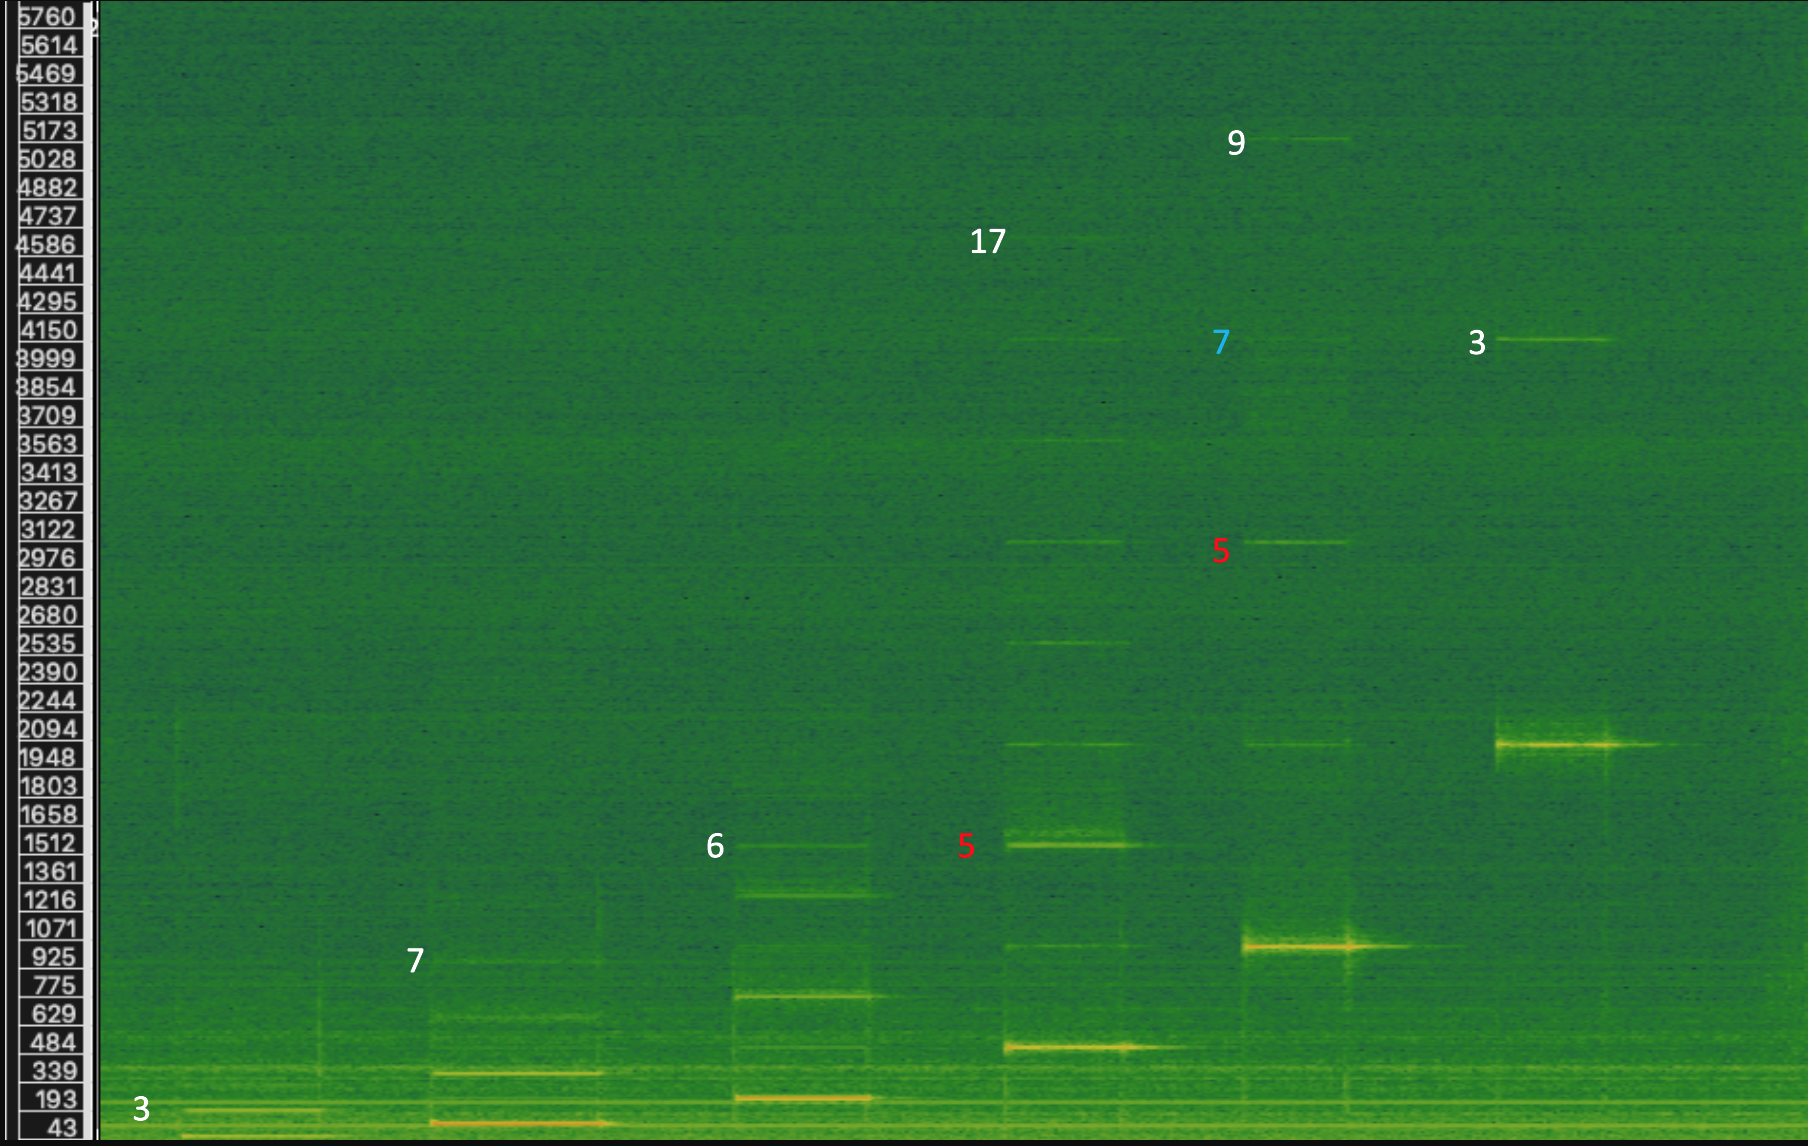
\includegraphics[scale=0.23]{bourdon}
    }
	\caption{Analysis of the note C in every octave of the 8' Bourdon of the Récit division using Sonic Visualiser. White numbers represent the number of harmonics present in a note, a red number represents a particularily strong harmonic, and a blue number a weak one.}
    \label{fig:bourdon_analysis}
\end{figure}

%%cmt Ajout d'analyse

In addition to emulating various organ stops, OrganLab permits what I call mutations\footnote{For a demonstration of several of these mutations, please refer to the file synthesis\_demo.mp4 that accompanies this thesis.}. 
The mutations of OrganLab are quite different from the tradition meaning of this term (a stop that sounds a note other than the key depressed, and refers to any process that alters an emulation.  
In fact, there are theoretically limitless mutations, but for a few examples: continuous pitches (glissandi); interpolation from one stop to another; decoupling of harmonic and transient content; and dynamic envelopes. 
These mutations allow me to fulfill my second and fourth aesthetic priorities, extending the organ's soundworld in a way that can be seamlessly navigated. 

%%cmt Ajout de précision et de la fluidité de l'écriture

\subsection{Live processing and effects}

The second modality, live effects, provides a simpler way of integrating with the sound world of the pipe organ, recording the sound with a microphone rather than reconstructing it from scratch. 
Extending the sound world is then a matter of applying any imaginable effect to the microphone's signal. As mentioned earlier, this provides a convergent mapping, and from an aesthetic perspective, I felt that adding effects to a pipe organ, essentially treating it like an electric guitar, would immediately situate it in a paradigm that would not normally be associated with the organ or a sacred setting\footnote{For a demonstration of several live effects, please refer to the file effects\_demo.mp4 that accompanies this thesis.}.

I chose to use Ableton Live instead of python for its robust plugins, my familiarity with the software, and to ensure the specificity of the role of OrganLab. As of the writing of this paper, I have explored reverb, distortion, and delay, but in the future it would be interesting to try other effects such as chorus, phaser, and pitch shifting. 

\subsection{Fixed media}

The use of prerecorded material is a controversial subject in hyper-instrument design.
As Palacio-Quentin puts it, “L’idée de jouer avec des sons électroacoustiques fixés est forcément contraignante pour une musicienne improvisatrice habituée à la liberté.” \footcite[50]{palacio-quintin_composition_2012-1}
At the same time, in an environment where the performer is juggling many things at once, triggering a sound file can free up the hands to perform other tasks, adding textural density and timbral complexity that would be hard to achieve by other means. 

%%cmt Correction orthographique

Furthermore, implicit in fixed media is an atemporality, allowing access to the past, memory, and alternate spaces.
The more time I spent in l'église Saint-Édouard and the more I considered its heritage and all of the shared memory inside and outside of its walls, the more it felt compelling to integrate a non-live component.
The interface for triggering these audio files is fairly straightforward.
I use a small MIDI keyboard to my left, and the chromatic keys step through the triggers sequentially.
In addition to playing audio files, loaded as clips in Ableton Live, these triggers are responsible for changing settings for effects and OrganLab, and initiating automations. 
In the piece \textit{Élégies}, there are two moments in the piece where it is necessary to trigger sound files at a distance, which is done through OSC using my phone.
I will discuss these choices as well as the poetic implications in greater detail in the following chapter.

%%cmt Changement de bed track à « fixed media » ou « sound recordings » pour plus de clarté. Suppression des informations non-nécessaires

%%cmt Correction orthographique

For the triggering of these sound files, I use Ableton Live. 
The sound files are organised into the clips of two tracks, to allow for certain sound files which overlap others, and are triggered as scenes using MIDI. 
Originally I used OSC, but found during a test performance during les journées de patrimoine of 2023, that the OSC was simply not reliable enough to be a sole solution. 
Ulimately, I still made use of OSC, using Touch OSC on my phone, for moments when I am no near the interface, but otherwise I used a small Akai keyboard sitting to the left of me on the organ bench.

\section{Diffusion}

The sound is diffused through five speakers that are placed throughout the church (see \cref{fig:stageplot}).
Speaker one is placed near the organ in the north transept tribune, on the left side, and is used mainly for synthesized sounds, which use only this speaker, in order to establish an instrumental synergy between the acoustic and synthetic organ.

Speaker two and three are the house system of the church, and are on the left and right sides of the choir, respectively. 
They are used mainly for playing pre-recorded sounds.
On the one hand, this creates an immersive, stereo experience of these sounds, and on the other, highlights their atemporality by associating them with the most visually prominent area of the church, void of human presence.
This also has a sacred implication, invoking timelessness while centering the sound around the alter.

Speaker four is positioned in the opposing tribune in the south transept, and is used for live effects.
This has a very practical purpose, which is avoiding feedback.
In a resonant space such as the church, it is difficult to avoid feedback when using delay-based effects, and so placing the speaker as far as possible from the microphone is useful.
From a poetic perspective, this opposition creates a tension between the acoustic organ and its processed sound. 
This is particularly evident when delay is applied, as the resultant echo is clearly differentiated from the sound source.
In terms of architecture, the church being symmetrical on the east-west axis, the south and north transepts can be seen as mirrors of eachother, the echos representing an inner communication and a deeper echo through history.  

The fifth and final speaker is located in the west gallery, and is the only one that is not connected to my computer.
This is due to both the impracticality of wiring XLR cables over the distance between the organ console and the west gallery, and the four output limit of my audio interface.
Instead, a Bluetooth speaker is used, which is controlled by a helper that plays audio off of a cell phone.
Though this speaker is less flexible and not directly integrated with the others, it was important to me to highlight the unique heritage of the organ of l'église Saint-Édouard and its history of relocation mentioned previously. 

%%cmt Reformulation de la déscription de la diffusion sonore au temps présent, et sans décrire les autres options considérées.

\customincludegraphics[scale=0.27]{stageplot_ste-edouard2}{fig:stageplot}{A view of l'église Saint-Édouard from above, showing the microphone and five speaker diffusion layout in relation to the organ console and the organ itself.}

\chapter{Creative approach}

\epigraph{\textit{What these histories so fundamentally reveal is that the performing arts are really an instable mixture amalgamating light, space, sound, image, bodies, architecture, materials, machines, code, and a perceiving public into unique spatiotemporial events.}\footnotemark}{}
\footnotetext[1]{\cite[xxii]{salter_entangled_2010}}

The construction of a hyper-instrument is no easy task.
As we have seen in the previous chapter, there are many theoretical questions and technical challenges that present themselves along the way.
This creative chasm is rivalled, however, if not dwarfed, by the realm of creative possibilities presented in the application of this interface, once constructed.
The structure of this thesis attempts to provide a neat narrative, chapter by chapter, going from historical context, to interface design and construction, and finally ending with creative application.
The reality of the process, however, has been anything but linear, and all three of these components have informed and directed the others in the course of this research.

In this chapter I’ll take the perspective of a composer and a performer as much as possible, imagining that the interface was designed by a third party, and is something that I’ve received and have to contend with.
I’ll attempt to describe not only the technical constraints of the interface, but the aesthetic implications of my work, and the tools that I used to explore it.

\section{As a performer (physical constraints)}

As far as the issues of interacting with the interface from the perspective of a performer, there are plenty of new obstacles to overcome and integrate. 
As a relative newcomer to the pipe organ in general, the traditional acoustic instrument already provides a significant challenge, and when I started playing the pipe organ at l’église Saint-Édouard, I found enough difficulty in playing the instrument as it was that I was intimidated by taking on the additional challenge of the augmented component. 
I nevertheless began to incorporate little by little the practice of managing the fourth keyboard. 

Having a fourth keyboard may seem trivial after already traversing three manuals and a pedalboard, but the principal challenge was the angle. 
Whether at the piano, the harpsichord, or the organ, a keyboardist will generally place themselves somewhere near the centre of the instrument, facing it directly. 
My original plan was to place the keyboard underneath the others to maintain this continuity of angle, but it quickly became apparent that there was not enough space to make this feasible, and the idea was born to place the keyboard off to the side. 

Besides the issue of keyboard angle there are also the issues of sustain pedal, patch changes, sample triggering, and volume control. 
The MIDI keyboard permits the pianistic privilege of the sustain pedal, which is not found on a traditional pipe organ, and is particularly useful for drone sections where one can simply depress the damper pedal, freeing the hands to do other things. 
One of the things that the hands might be freed up to do, besides playing the other manuals or changing the registrations, is triggering samples or regulating the volume of the synthesized sounds. 

\section{Expanded practice}

Until now I've been speaking of the pipe organ as an instrument. 
That is to say, an interface, with keyboards that receive gestural data and pipes that radiate sound to the listener. 
At the outset of this project I intended to focus on this instrumental perspective, expanding the timbral possibilities with synthesis.

While creating \textit{Élégies}, however, it soon became clear that the space itself was integral to the context of the instrument. 
The pipe organ is unique in this regard, being not only an instrument, but a permanent architectural installation. 
Hans Fidom makes this case, claiming that “If there is one form of music which is explicitly situational, certainly within our Western culture, then it is organ music.”\footcite[23]{fidom_music_2012}. 
L'Huillier and Machover use architecture as a metaphor for music itself\footcite[361]{lhuillier_spaces_2018}. 
This fundamental connection to the sacred space of the church was too compelling to ignore, and soon inspired me to look for ways to expand my artistic vision of the piece beyond a straightforward instrumental perspective, pursuing a `sonic architecture'\footnote{“Sonic architectures are intentionally designed architectural soundscapes that create the conditions for the emergence of a building’s Voice” \footcite[2]{lacey_site-specific_2014}.}.

I call this approach an expanded practice, and in the following sections I'll describe several ways in which I explore this expansion.

\subsection{Spatialisation}

Firstly, the sound diffusion discussed in chapter two was a way for me to play with the fullness of the space. 
In this way, a listener hears not a unified sound source coming from the organ, but a wide variety of sources surrounding them. 
Each source has a poetic significance. 
The synthesis comes from the same direction as the pipe organ in the tribune of the north transept, aligning with Palacio-Quintin's ideal of a unified instrumental experience.

The effects come from the opposing, south transept tribune, implying a dialectic between the instrument, and its transformation, or in the case of the delay effect, an echo. 
The echo is perhaps the most cogent effect from a poetic perspective, as it evokes the sacred traditions of antiphony and call and response, while implying the echo of history. 
The echos create a feedback where each iteration becomes quieter and quieter, similar to how the further we move into the past, whether collectively in terms of history, or personally in terms of memory, the more veiled and inaccessible. 
Another metaphor is the mirror. 
I imagine the organ as the protagonist, facing a distorted reflection of itself.

\subsection{Fixed media}

The other sense in which I attempt to embody the richness of l'église Saint-Édouard is through the use of prerecorded audio, and in particular through what I call \textit{le chemin}, a reference to \textit{le chemin de croix}, or in English, the stations of the cross. 
In English we emphasize the moments in the fourteen stages of Christ's crucifixion, yet in French, we emphasize the movement between them---the journey itself. 
My piece also represents a journey, both musically and dramaturgically. 

Throughout the piece are heard audio recordings in various areas of the church, including outside the church. 
During my master's program, in addition to being organist, I also became caretaker at l'église Saint-Édouard, allowing me access to the many areas of the church that would not be otherwise accessible. 
I used this privilege to take audio recordings not only the sanctuary, but various places throughout the building. 
The general narrative of the path is that the subject walks towards the church as the bells sound in the distance. 
She then enters the church through the basement, moving past the compressor room in la salle Saint-Édouard and through la salle Morin, eventually coming to the furnace room. 
In my mind, the furnace room represents the bowels of the church---a key moment of darkness in the narrative structure. 
At the same time, the ominous sound of feedback in the church, throbs incessantly in the background. 
Later a match is struck, referring both to the candles that burn day and night in the church, as well as to the darkness of the path being walked. 
Finally, the sound of rain enters with the same sound of bells from the beginning of the piece, but in reverse. 
The last tableau is the sound of the subject walking up the steps from to the organ balcony, accompanied by the sound of pigeons.

The reason that I call this path symbolic is that first of all, like a photograph, it is not the experience itself, but a representation of that experience, but furthermore, the sound recordings heard throughout the piece were not captured on the same day, and are not continuous through the space, at times juxtaposing several different spaces at once. 
This presents not a real path through the church, but an imagined one that escapes temporal and spatial bounds.

In the following sections, I'll outline the different stations of \textit{le chemin}, in order of their appearance in the piece. 
Rather than fourteen, there are seven, with each recording representing different places in and outside of the church. 
Sometimes these recordings are used as linking material between movements, and sometimes they are heard during a movement.

\textbf{First station} (00:00--01:30)\footnote{Included timestamps are for elegies\_video.mp4}:

\begin{figure}[h]
    \centering
    \subfigure{
        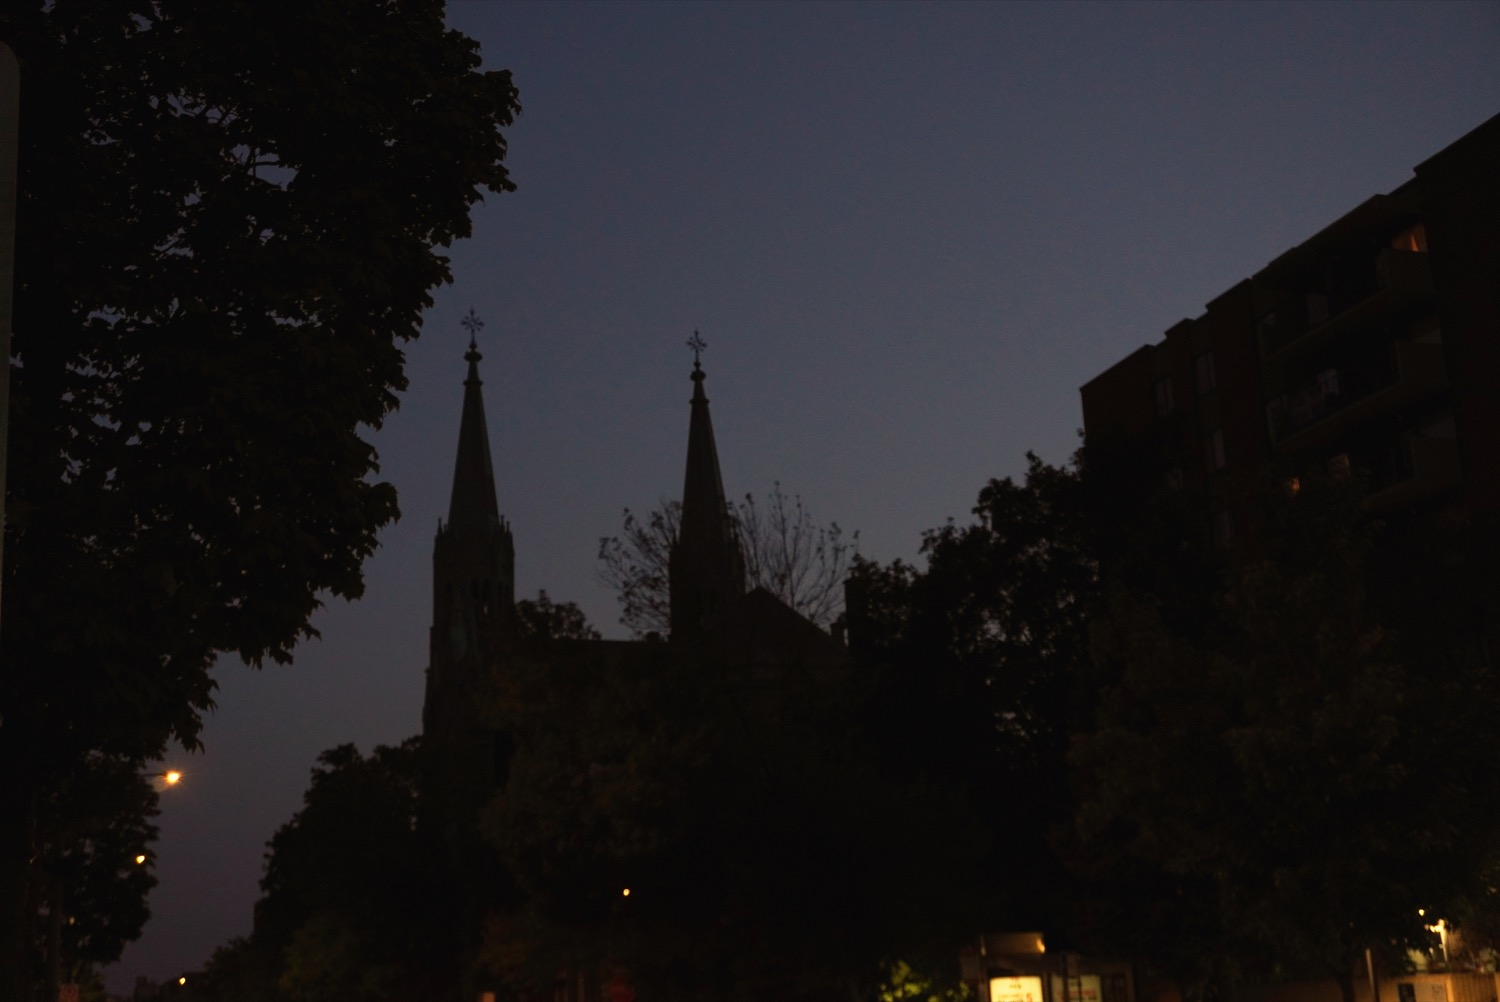
\includegraphics[scale=0.14]{DSC00200_1}
    }
    \subfigure{
        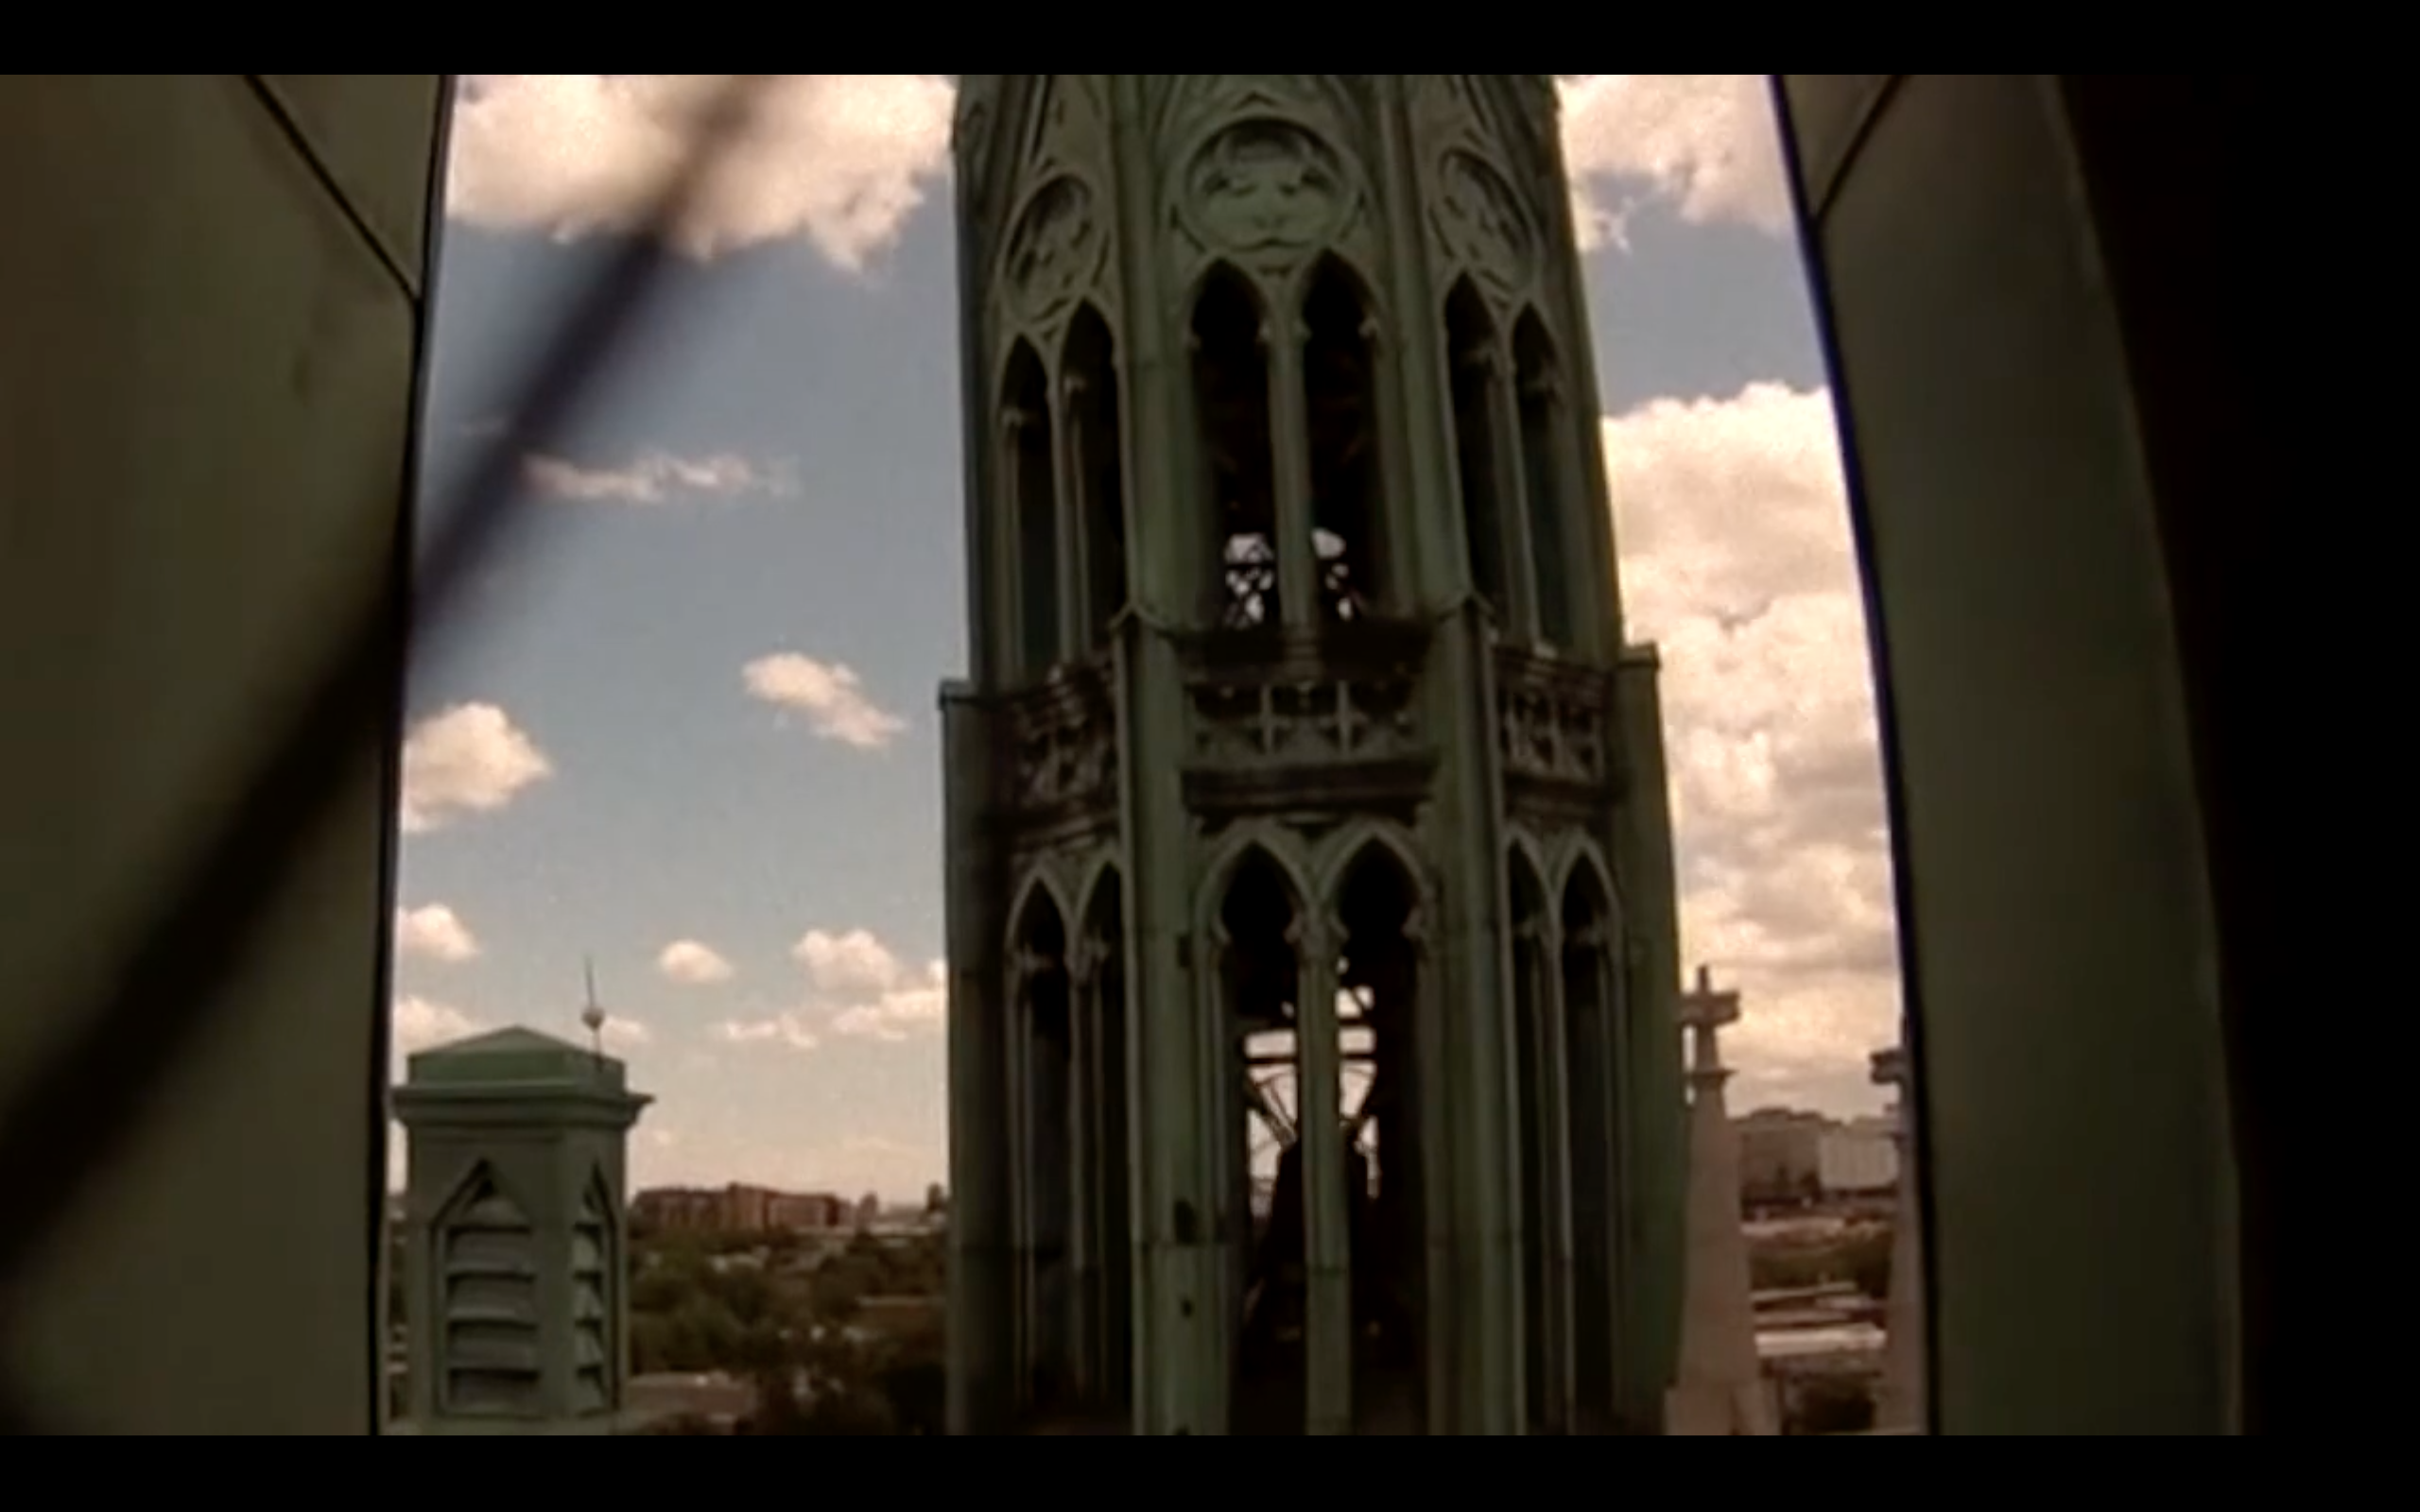
\includegraphics[scale=0.15]{eglise_youtube2}
    }
    \caption{L'église Saint-Édouard from la rue Beaubien on the left, and the footage from the YouTube video on the right.}
    \label{fig:station1}
\end{figure}

The first station opens the piece, and is a combination of two recordings. 
On the one hand, a recording of me walking down Beaubien from my apartment to l'église Saint-Édouard during the summer rain storms of July 2023. 
This is layered with another recording that I downloaded from the YouTube channel \textit{Saint-Edouard de Montréal} of the bells of l'église Saint-Édouard\footcite{saint-edouard_de_montreal_volee_2022}. 
This latter recording was distorted with the plugin Chow Tape Model and treated with the Spectral Blurring plugin by Michael Norris\footnote{These effects become less and less pronounced, to give the impression of a distant sound becoming nearer}. 
These recordings, especially that of the storm, place into question the distinction between inside and outside. 
The church is a contained unit, which is often heavily sonically isolated from environmental sound, especially with stone constructions like l'église Saint-Édouard. 
By using audio recordings from the outside of the church within these confines provides a rare experience of hearing the external from within, as if this sacred boundary had been dissolved.

%%cmt Correction orthographique

\textbf{Second station} (06:19--06:40):

\customincludegraphics[scale=0.15]{DSC00149_1.JPG}{fig:station2}{The compressor room upon entering the basement of the church.}%%Station 2

The second station is a recording of entering the church through the basement of the church, and entering the compressor room (\cref{fig:station2}). 
This is the room that stores all the compressors and valves that connect to the elaborate sprinkler system throughout the church. 
I found that this room emitted an interesting electrical hum, and seeing as it is right beside the entrance on Beaubien, it seemed fitting to begin the journey inside the church at this point.

\textbf{Third station} (18:18--18:47):

\begin{figure}[h]
    \centering
    \subfigure{
        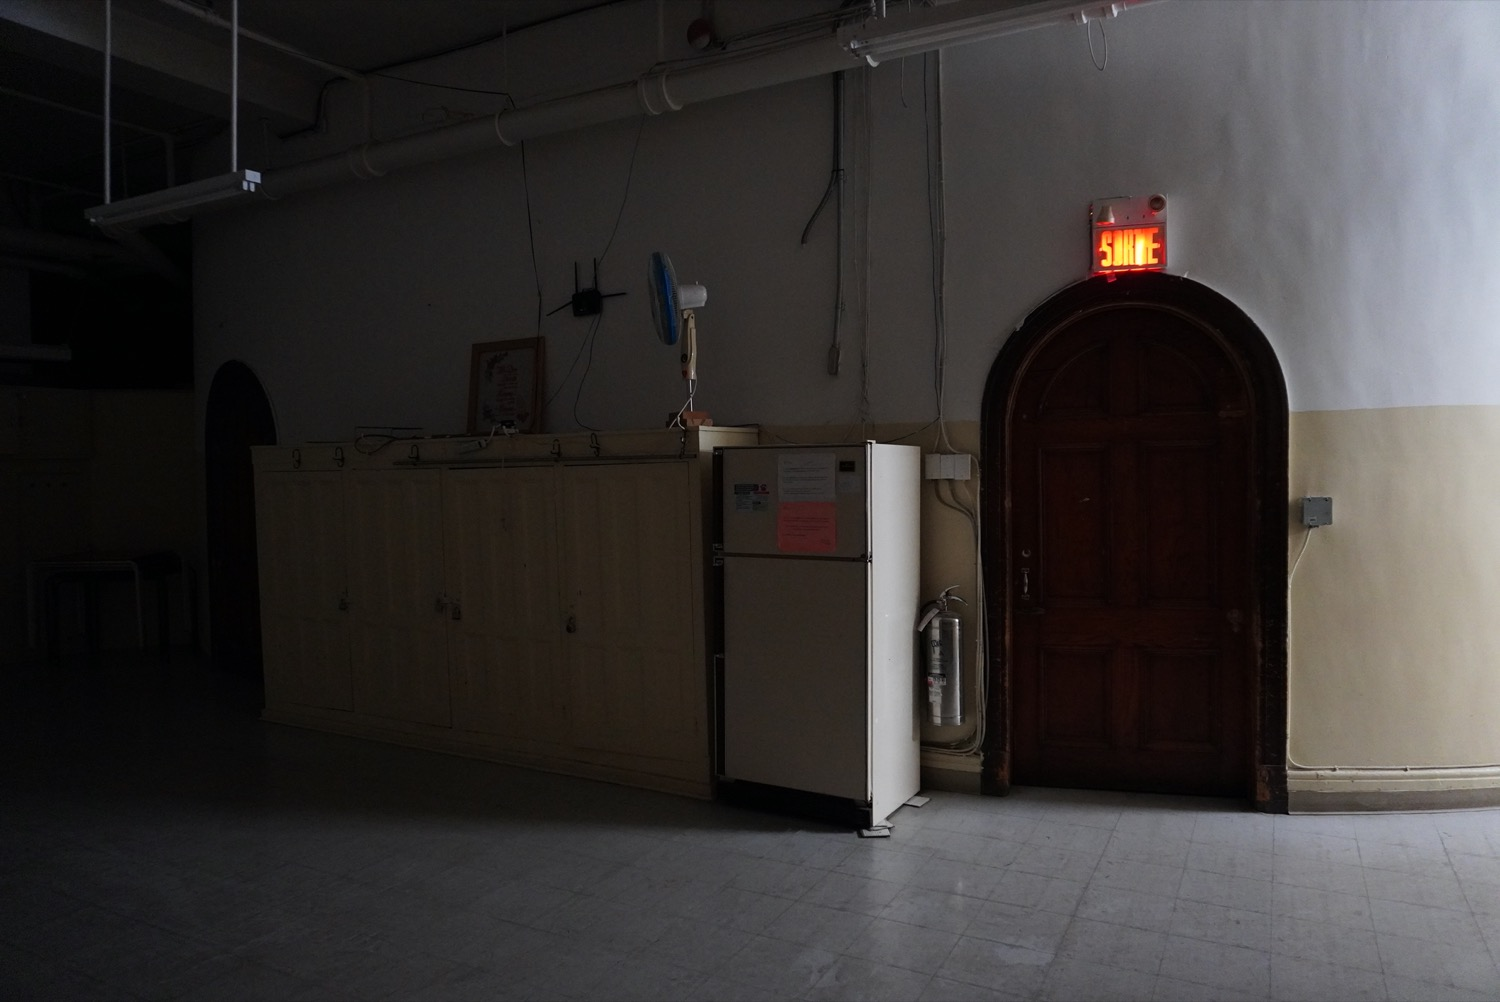
\includegraphics[scale=0.15]{DSC00123.JPG}
    }
    \subfigure{
        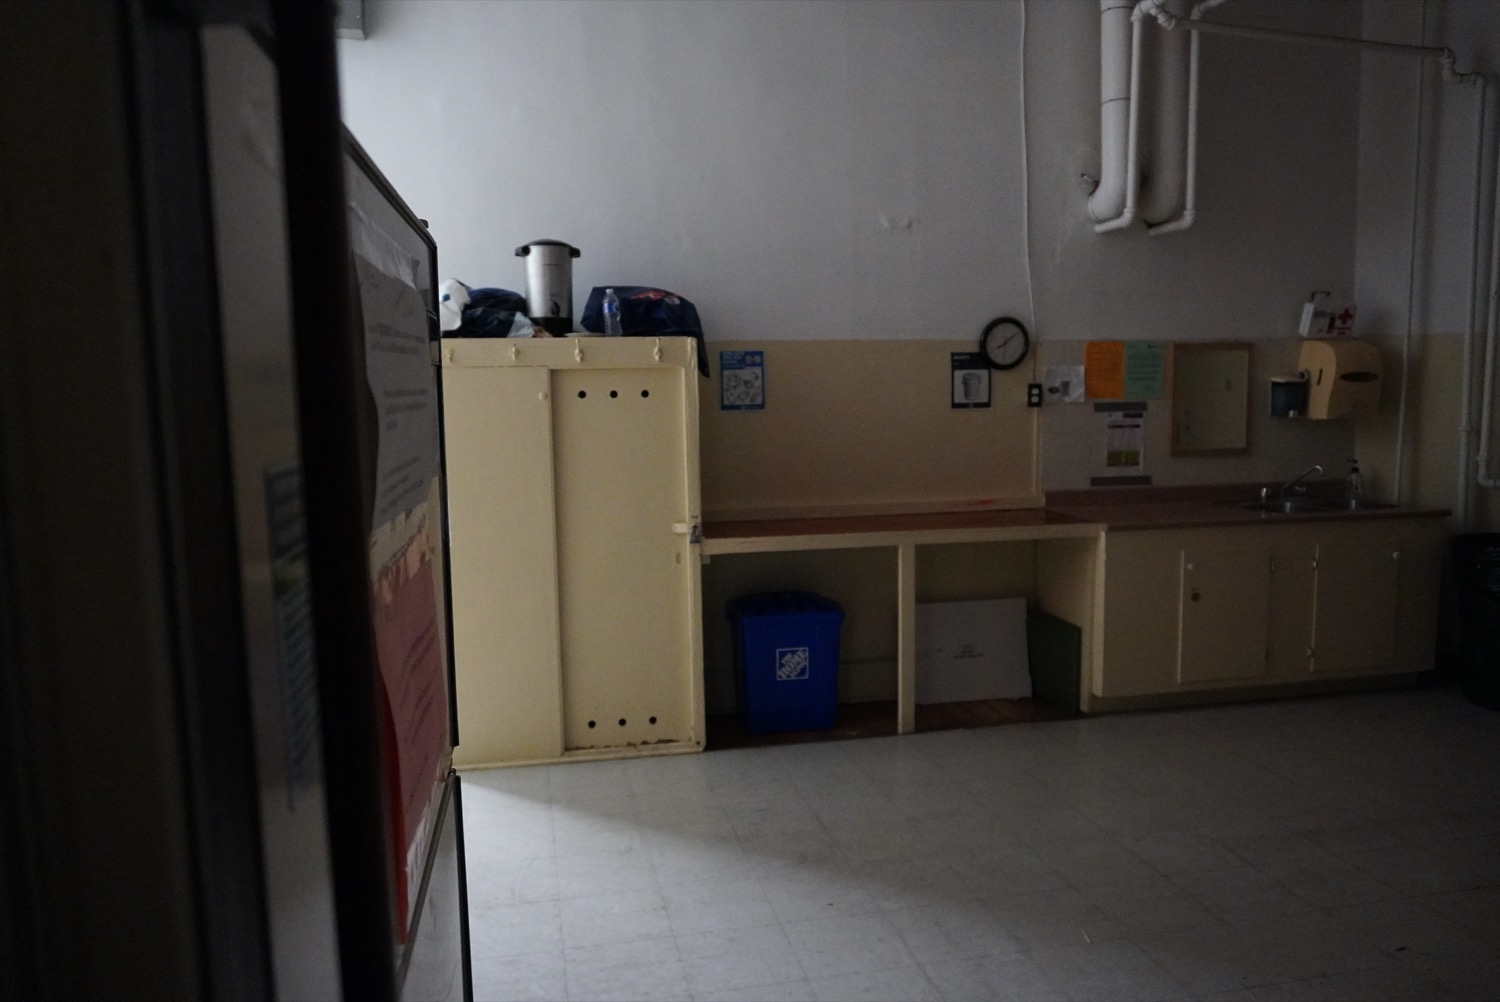
\includegraphics[scale=0.15]{DSC00136.JPG}
    }
    \caption{The fridge of the salle Morin pictured on the left, and the clock viewed from the fridge on the right.}
    \label{fig:station3}
\end{figure}

The third station takes place in la salle Morin, a hall that is very frequently rented for events, and is named after the first priest of l'église Saint-Édouard Joseph-Napoléon Morin in 1895. 
This space has two unique sonic features: a dissonantly humming fridge, and a ticking clock (see \cref{fig:station3}. 
Here I play with the unique lens of subjectivity that the microphone provides. 
Elsewhere in \textit{le chemin}, often I am holding the microphone as I walk, providing a close representation of my subjective aural experience, but in the third station, I leave the microphone on the fridge while I leave the room. 
This recording is then crossfaded with another recording where I move the microphone closer and closer to the ticking clock. 
At the same time, I double the sound of the clock, with a time offset, creating the sense of fracturing of time, while my footsteps recede into the distance.

\textbf{Fourth station} (27:59--43:34)\footnote{Timestamps for fourth and fifth stations are harder to pinpoint as the two are juxtaposed, and elements of each are present throughout a long duration. Though the sounds of the furnace feature prominently only towards the beginning of the recording, from a narrative standpoint I place the protagonist in the furnace room for a longer duration.}:

\customincludegraphics[scale=0.15]{DSC00157.JPG}{fig:station4}{The metal sliding door of the furnace room. When the recording took place this door was burgundy, but it has since been painted white.}%%Station 4

The fourth part of \textit{le chemin} begins in the furnace room. 
This room has a fantastic sliding metal door (Depicted in \cref{fig:station4}) that creates a loud, foreboding sound when opening or closing it. 
This sound opens the seventh movement, which is the only movement that is wholly electroacoustic. 
Furthermore, this is the first time in the piece where two different spaces are juxtaposed. 
By placing the listener simultaneously in the furnace room and in the church, there is a dreamlike, disorienting element, if not directly experienced, as the listener will not recognize the places of recording without prior knowledge, at least at a poetic level.

\textbf{Fifth station} (27:59--43:34):

\customincludegraphics[scale=0.15]{candles.JPG}{station5}{The ever burning candles of l'église Saint-Édouard flicker in the darkness.}%%Station 5

The fifth station marks the entry into the church itself. 
Sonically, this is referenced with three recordings: the sound of a match being struck, symbolizing the candles seen in \Cref{station5}; the sound of feedback resonance that appeared mysteriously while testing high decay reverberation effects (this will be discussed in detail in the section on the seventh movement in chapter four); and the sound of running footsteps. 

\textbf{Sixth station} (43:34--47:25):

\customincludegraphics[scale=0.15]{eglise_mh.JPG}{station6}{The bell towers whose sound features prominently throughout the piece.}%%Station 6

The sixth station continues the previous station's reference to the opening sounds of the piece. 
Another sample of the July storms of 2023 are heard, this time with an emphasis on the rain rather than the distant thunder sounds featured in the opening recording. 
Later on, this rain sound is crossfaded into the same bell recording from the beginning of the piece, this time in reverse. 
This reversal of time provides a poignant reference to the theme of transcendence evoked by Rilke's final elegies, while creating a sense of aesthetic unity in the piece.
At the same time, this station is the most abstract, not representing a specific space, but moreso the idea of ascension.
I see the view of the city from the bell towers as the rain falls.

\textbf{Seventh station} (47:55--49:10):

\begin{figure}[h]
    \centering
    \subfigure{
        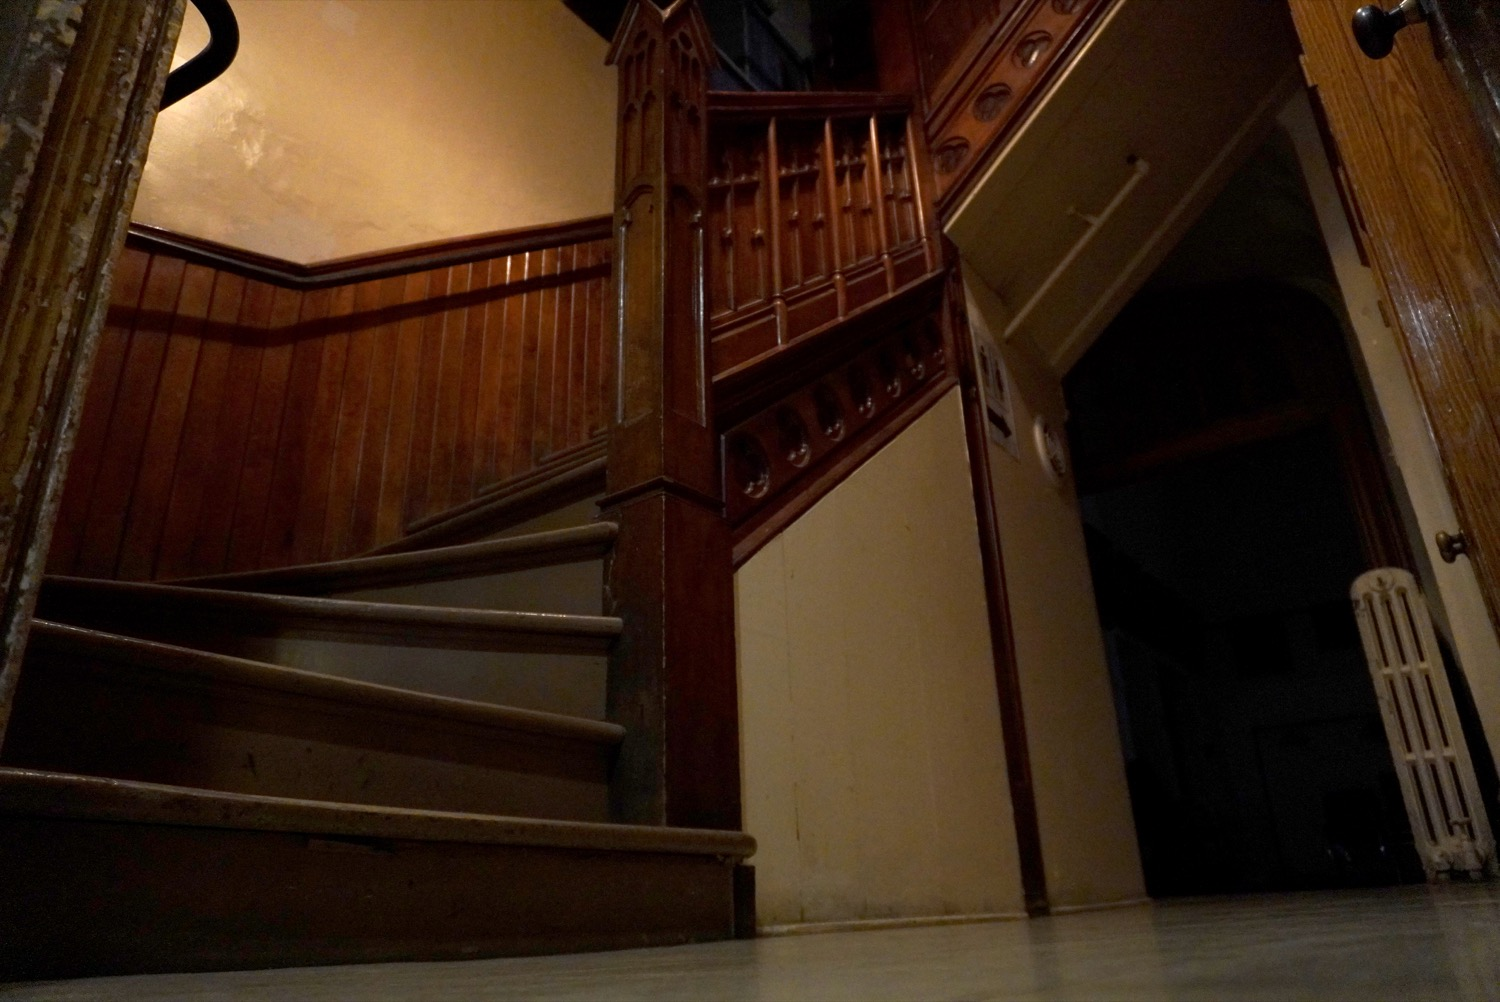
\includegraphics[scale=0.15]{DSC00117_3}
    }
    \subfigure{
        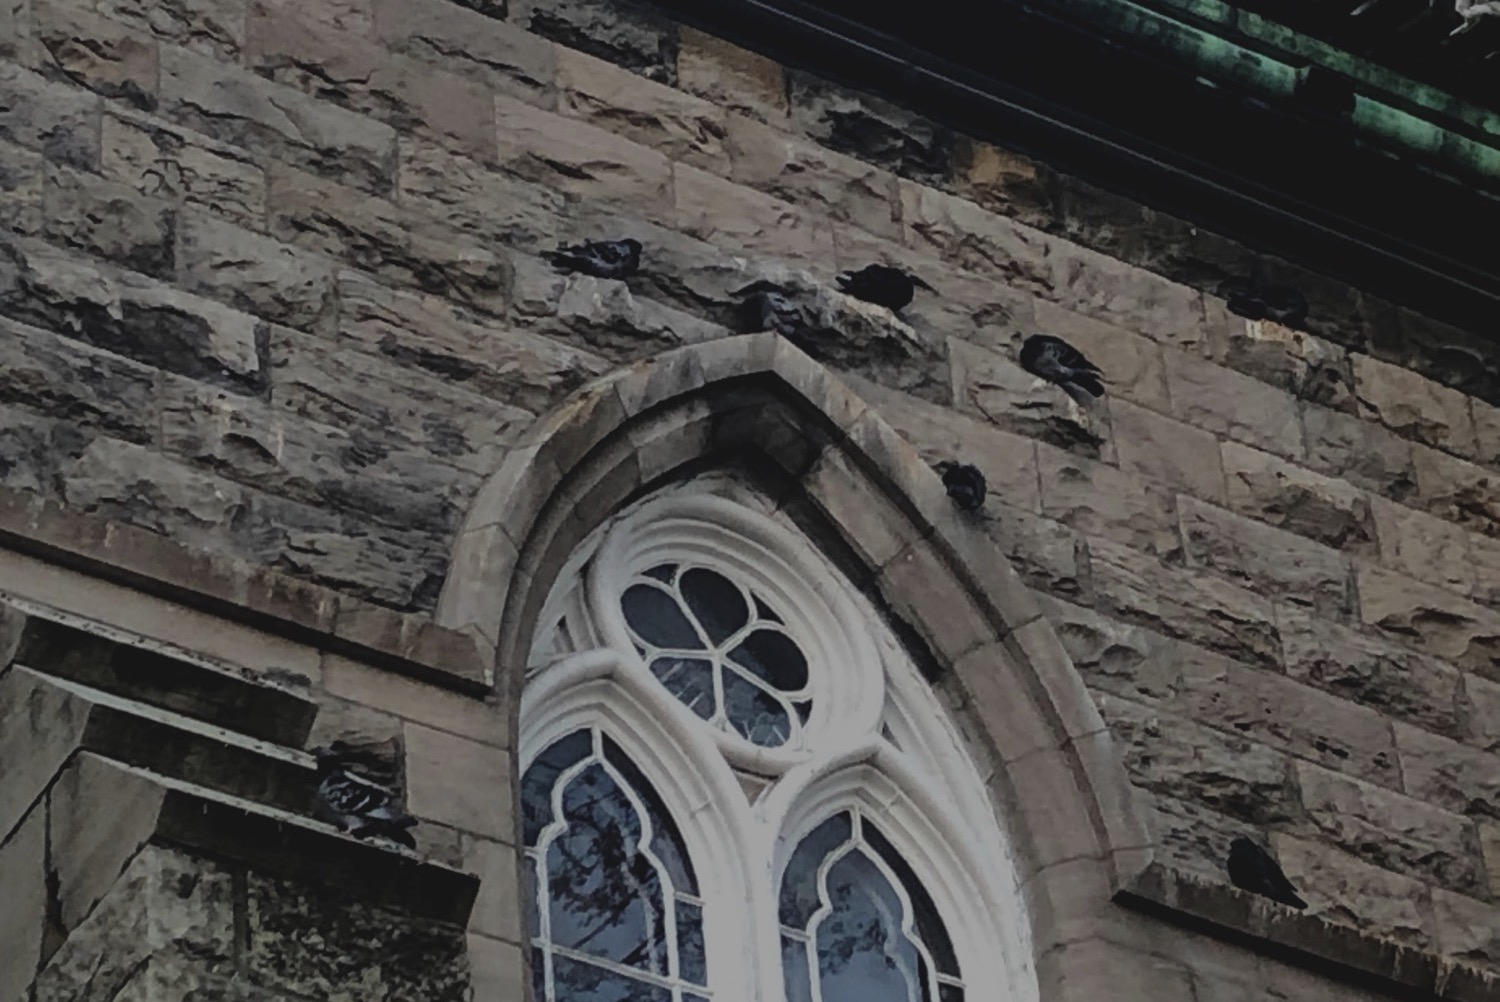
\includegraphics[scale=0.15]{pigeons}
    }
    \caption{The stairwell leading to the organ loft on the left, and the pigeons of l'église Saint-Édouard nestled into the church's stone walls on the right.}
    \label{fig:station7}
\end{figure}

This station is in two parts. 
The first is a recording of me climbing of the stairwell leading to the organ loft (pictured in \cref{fig:station7}, which symbolizes the ascent from the furnace room, which is connected to the organ loft stairwell through the mezzanine
This creates a link to the beginning of the piece, which begins by my entering the organ loft from the stairwell. 

This recording is layered with the sounds of pigeons, which is informed by by my first experience with l'église Saint-Édouard, almost a year prior to my becoming organist there. 
I was walking with my friends Marie-Hélène and Francis, and as we passed the church, admiring its beauty, Marie-Hélène stopped to take photos of the many pigeons who call the church their home (depicted in \cref{fig:station7}). 
The sound of pigeons is an ever present part of the Saint-Édouard soundscape, and the flight of these gentle birds parallels the ascent of the stairwell, adding to the spirit of transcendence while offering a more interesting timbral profile than the sound of the steps on their own. 

I used the sounds of their cooings and flutterings, layered, and gradually slowed down, against the slowed recording of my footsteps ascending the stairwell, each fluttering becoming progressively longer.

\subsection{Voice}

Another aspect of \textit{Élégies} that can be grouped under expanded practice is the use of the voice. 
Voice and organ is hardly a unique pairing, but it is unusual for the organist and singer to be the same person.
The centrality of the juxtaposition of the organ and the voice plays a narrative function, placing in contrast two very different paradigms.
The organ as the discrete and technological\footnote{This position is echoed by Bela Bartok's classification of the pipe organ as being more mechanical and less human.\footcite[24]{jorda_digital_2005}}, with its distinction between the control interface and the sound production, and the voice as continuous and natural, with the control mechanism and sound production indistinguishable. 
Ironically, we can say that the voice is organic, while the pipe organ is inorganic.
 
This juxtaposition is eventually resolved.
Initially appearing individually, towards the end of the piece, they are brought together and heard simultaneousy.
This `singing while playing' is typical of other keyboard instruments, but less so with the pipe organ, adding a singer-songwriter element that draws the ear towards more pop\=/oriented references.

%%cmt Ajout d'une section sur la voix en terme de "Expanded practice"

\section{Aesthetic references}

Here I'd like to outline some of my major aesthetic influences and considerations that shape my approach to making art. 
One of my formative musical experiences was hearing “Everything You Do Is A Balloon” by Boards of Canada on late night CBC radio as a teenager. 
This group's use of archival audio and imagery was my first introduction to music that seemed to be about the past. 
Since then I've discovered other artists who take this approach, especially UK artist Burial. 
His music, especially his first two full length albums, and a 2012 interview with Mark Fisher where he describes his creative perspective, deeply influenced my own \footcite{fisher_burial_2012}. 
In his music, one get's the sense that he's not creating an experience, so much as describing one. 
Rather than the club itself, the sound of the club in the distance, or the memory of it echoing in one's head while walking home. 
Both Burial's attempts to communicate his imagined experience of UK rave culture that he was too young to experience, and Boards of Canada's re-imagining of their childhood in Alberta can be described as a form of hauntology \footcite{alary_vers_2020}.

At the same time that these meditations on the past fascinate me, I've also been influenced by a pursuit of `liveness'. 
The first time that I listened to the music of Arca, for instance, I had the impression of an immediacy---that the music was somehow a living, breathing organism. 
This is a very different approach from the former, and highlights an important tension in my thought. 
I explore this tension through the mixing of live performance and pre-recorded sound files, the combination of the organic the inorganic, and the use of both traditional and modern stylistic references.

Embedded in the question of liveness, especially in a concert context, is the issue of presence. 
Often, performers, instrument designers and composers prioritize clear, comprehensible gestures in order to make the physicality of performance explicitly communicable. 
In my own work, I'm just as interested in the subversion of these expectations, calling into question the nature of shared space. 
By exiting and re-entering the view of the audience, including gestures that do not have a sonic result, as well as sounds that do not have a corresponding gesture, we engage in a play of shadows---a commentary on information loss and incommunicability. 

\section{Tools}

Before entering into the analyses of the work itself, I want to make a brief mention of the various tools that I've used in the construction of Élégies. 
Besides my own software OrganLab, which I mentionned in the previous chapter, I've used several tools to help investigate, test, sonify, and notate my compositional ideas, without which the writing of this piece would be simply not possible. 
First of all, Ableton Live was used not only in a performance context to trigger sound files, apply real-time effects and manage spatialisation as discussed in the previous chapter. 
It also served as an indispensable tool for arranging my improvisations and compositional ideas so that I could envision the macro structure of the work. 
I also used Ableton Live for the sound design of all the soundfiles used throughout the piece. 
Reaper was also used to batch slice and export the samples used for the beat towards the end of the piece.

Another essential piece of software was MuseScore. 
MuseScore was used to express my ideas in notational form, allowing me to gain distance from my improvisations and form the material without my physical constraints, leading all the way to the finished score, created with a single .mscx file. 
In order to audiate my ideas, I originally used MuseScore's built in pipe organ sound. 
Eventually exasperated by this wholly uninspiring playback, I investigated alternatives, ultimately discovering Grand Orgue. 
In the summer of 2023, I created a custom .organ file for GrandOrgue based on the Burea Church organ, which was made to mimick the both the layout of the stops of the organ at l'église Saint-Édouard, as well as the corresponding stop sounds as close as possible. 
I did this by combining stops that I felt similar from various different virtual pipe organs, creating a frankenstein organ whose stops draw from a wide range of epochs and building styles (see \cref{fig:grand_orgue}. 
Eventually, it would be wonderful to sample the stops at l'église Saint-Édouard and create a virtual organ representing this space, but for the purposes of creating MIDI mockups, this was already leagues ahead of MuseScore's built in sounds. 
I followed an excellent Virtual Pipe Organ (VPO) guide by Jester Musician on the MuseScore forums to implement GrandOrgue into MuseScore 3 using a custom instruments.xml file and Staff Text Properties to manage registration changes \footcite{musician_jester_how_2018}. 
I was even able to drive and manage the cues in OrganLab and Ableton Live with this same .xml file. 
Unfortunately, as of my last attempts with MuseScore 4 in early 2024, it still does not support this VPO integration, and so I've been using MuseScore 3 until this is available.

\customincludegraphics[scale=0.3]{grand_orgue}{fig:grand_orgue}{My emulation of the Saint-Édouard organ, mimicking its console and borrowing stops from several different organs.}

I will make a special mention of OpenMusic for helping me to explore some more technical solutions outside of my cognitive computational ability. 
Though I didn't ultimately implement much of these experiments into the final score, it was nevertheless a useful way to workshop my ideas that I look forward to exploring more deeply in the future.

\chapter{\textit{Élégies}}

\customincludegraphics[scale=0.2]{2024-04-28_MH}{fig:live}{The artist during concert preparations for the first performance of \textit{Élégies}}

In this chapter I will detail the construction of the piece \textit{Élégies} movement by movement, including the process of interpreting Rilke's poetry in a musical\=/narrative framework, the various materials and techniques, both compositional and digital, that are employed, the form of each movement, as well as issues of dramaturgie and staging. Before we begin, I will briefly describe my general approach to selecting and interpreting Rilke's texts. First of all, throughout this process, I did not consult any third party texts on the \textit{Duino Elegies} other than biographical information about Rilke. This was an intentional choice to allow the space for a genuine, personal reading that was not influenced by other analyses. This may mean at times that my understanding is deeply flawed. I fully accept this likely possibility, and can only hope that Rilke would appreciate this imperfect expression. The version of the \textit{Duino Elegies} that I have used to form my interpretation and draw text from is a bilingual edition with both the original German text as well as a French translation by Armel Guerne\footcite{rilke_egies_1986}. Why set the French text and not the original? For one, I don't speak German, for another, I find that the French text, particularily Guerne's translation, is beautiful, metrically balanced, and euphonic.   

Of course, when setting any text to music, one has to make selections. 
With writing as dense as Rilke's, and in a context where instrumental music is featured prominently, this is only more so true. 
Initially, I considered setting lines throughout the texts, but ultimately, I found that the opening lines of each elegy were so striking, and seemed to outline a clear narrative, that I chose to use the first line of each elegy. 
Often, using the entire sentence was either impractical, unmusical, or less evocative, and I use incomplete phrases. 
Though my musical interpretations are informed by the \textit{Elegies} in their whole, my focus has been on rendering these poetic fragments\footnote{Several of these fragments are not set to music in their entirety, with one not sung at all, and another reconstructed. They are nonetheless quoted at the beginning of each movement analysis, serving as a narrative guide.}. 

I also want to provide some preliminary notes on the context in which this work was conceived. 
\textit{Élégies} was very much informed by l'église Saint-Édouard and my role as an organist and vocalist. 
As of December, 2024, it has been performed three times in its entirety this year, on April 26\textsuperscript{th} and 28{th}\footnote{The video file elegies\_video.mp4 accompanying this thesis represents the April 28\textsuperscript{th} performance, while the file elegies\_audio.mp4 splices in several moments from the April 26\textsuperscript{th} performance that were more successful.}, and again on September 7\textsuperscript{th}.
Each time was in l'église Saint-Édouard with me playing the organ, singing, and working the electronics.
While I am open to the this piece being performed in other spaces, by another artist, or perhaps two artists fullfilling the roles of organist and vocalist, it is nevertheless the case that this work has been created within a specific context. 
In the following analyses, I'll use both the first, and third persons (performer(s), organist, and singer) interchangeably. 
This is to acknowledge the reality of the origins of the work and the conditions of the first performances, while imagining a more generalizable approach.  

Finally, I'll comment on the implications of using Rilke's \textit{Elegies} in a sacred space. 
Though Rilke himself was not religious, and his \textit{Duino Elegies} are not based in a specific spiritual tradition, they are nevertheless replete with references to angels, saints, churches, and the ineffable\footcite[147]{gass_reading_2013}.
Central throughout these texts is a tension between the sacred and the profane---a theme that I seek to mirror in my own work. 

\section{1\textsuperscript{re} élégie\footnote{00:00--03:45 in elegies\_video.mp4}}

\epigraph{\textit{Qui, si je criais, qui donc entendrait mon cri parmi les hiérarchies des Anges?}}{Rilke, \textit{Les Élégies de Duino}\protect\footnotemark}

\footcitetext[9]{rilke_egies_1986}

\subsection{Narrative context}
Rilke's \textit{Elegies}\footnote{The title of the piece \textit{Élégies} as well as the movement names, follow French orthography in homage to the French translation that I used, but for ease of reading I will use the English form when referencing Rilke's texts, while referring to the musical elegies as movements.} begin not with a cry, but with the question of a cry--- a question seemingly addressed to no one.
Perhaps this question is addressed to God, to the reader of his poem, or to the protagonist herself.
With this opening line, Rilke evokes a profound spiritual solitude, placing into question the purpose of attempts to communicate.

From a sonic perspective, the issue of sound is immediately relevant, the cry evoking at once a sound source---the human voice---and the volume and intensity of this sound.
The subjective nature of sound is also essential, with “qui donc entendrait” illustrating the importance of hearing and perception to the auditory experience.
This startling juxtaposition between the immense loudness of the subject's inner world, and the expansive quietude of the environment, provides an immediate dialectic between inner and outer worlds.

The second part of the sentence describes the setting somewhat, though in obscure terms.
He depicts the subject as being among “the hierarchies of angels”, signaling another essential tension to Rilke's world: the spiritual versus the human.
Here is a startling image.
We were quickly led to believe that we were alone, contemplating the futility of communication, when not only are we not alone, but we are found among a cacophony of angels.
The reason that the angels might not hear the subject's plaintive cry is unclear. 
Maybe the angels are simply too far away.
Maybe they are making too much noise themselves to hear anything.
Or maybe they do not contain the capacity for subjective experience at all.
If we take this last case, this quickly paints an image of Rilke's angel, not as an idealized human, but as a very different creature entirely.
The idea that they would hear nothing implies an austere, cold distance from the angels---the small human alone underneath a swarm of ethereal beings.

\subsection{Materials and techniques}

One major advantage of a digital pipe organ over an acoustic one is the ability to use non-discrete pitches.
To represent the hierarchies of angels, I make use of an extended glissando, starting in a lower register and moving upwards, signifying a transcendent nature.

The glissando I employ here is not a traditional one. 
A more appropriate term would be `spectral glissando'. 
The way that this works, is that over the course of a set amount of time (in this case two minutes), the frequency of each of the harmonics is incremented by one about ten times a second (see \cref{fig:glissup}).
Because the frequency is being incremented, and not the MIDI cents, the sound quickly becomes inharmonic.
This process creates the sensation of an alien movement, pulsating and morphing, yet not in a coherent, familiar way.

%%cmt Précision de Hz

\begin{figure}[H]
\begin{lstlisting}[language=Python]
glissC = [0 for i in range(8)]
def glissUp():
    global glissC
    for i in range(len(glissC)):
        glissC[i] == 0
    if glissC[0] < 6
        stop1.setTrans(glissC)
        for i in range(len(glissC)):
            glissC[i] = glissC[i] + 2
    else:
        for i in range(len(glissC)):
            glissC[i] = 0
\end{lstlisting}
\caption{The glissUp function takes a python list and increments it until it reaches 600, this list is used to increment the first 8 partials of the synthesis module}
\label{fig:glissup}
\end{figure}

For this movement, I represent the binary form of the poetic fragment with a juxtaposition of proportional notation and semi-metric notation, with proportional notation representing the angelic form and metrical time the human.
This choice is somewhat arbitrary.
One could easily make the case that metrical time is more hierarchical.
At the same time, metrical time has a long tail of history in western notation, and has for me a notion of human comprehensibility, whereas proportional notation has less historical associations.
Furthermore, proportional notation seems to give the sense of music frozen and static in time, which I associate with the timelessness of the ethereal.

\subsection{Form and compositional process}

This movement begins with layered recordings of a walk through a storm and the Saint-Édouard bells, representing the first station of \textit{le chemin}.
This recording is triggered before the performer(s) arrive in the organ loft, either with OSC, or by a helper hidden in the organ loft that can access the MIDI keyboard.  
These sounds are passed from speakers one, two, three, and four, encircling the audience and creating the sensation of wind sweeping through the church. 
They enter gradually, building, and eventually looping the final portion to ensure that the ascent to the organ loft is not constrained to a specific time. 
Upon arriving at the organ and verifying that everything is well prepared, the performer simply presses the next key on the MIDI keyboard, the recording gradually fades out, and the melodic fragment depicted in \Cref{ex:1e_1} is sung.
This melodic fragment is adapted from a session of singing the poetry of Rilke in l'église Saint-Édouard in the fall of 2022\footnote{This was a solo session where I paced throughout the dimly lit church while searching for melodic material in the text. I recorded these experiments on my Zoom H4N and later sifted through them for the most compelling moments.}, and is developed throughout the rest of the piece.

%%cmt Ajout du contexte sur la séance d'enregistrement

\begin{example}[H]
    \centering
    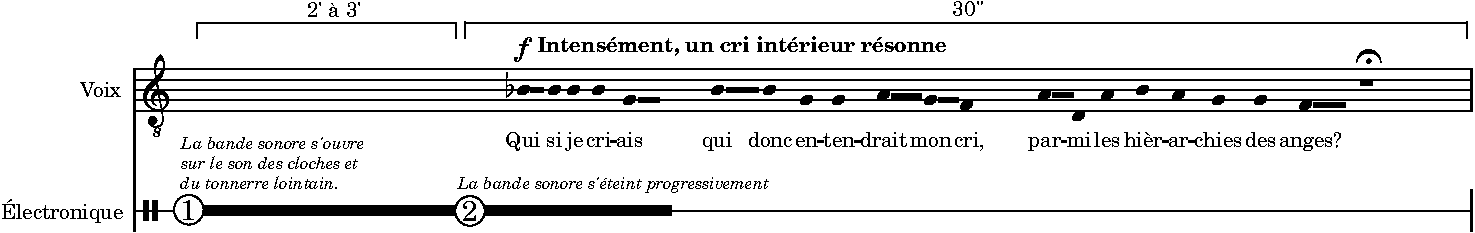
\includegraphics[width=\textwidth]{1e_1}
    \caption{The principal melody of the piece, based on the 19 syllables of the first line of Rilke's Elegies (p.~1, sys.~1)\protect\footnotemark.}
    \label{ex:1e_1}
\end{example}

\footnotetext{In all excerpts in proportional notation, accidentals carry to the end of the system.}

Then comes a sonic interpretation of the cry---the internal, subjective cry.
Of course, there is no correct, objective way to represent subjectivity, but I've attempted a poetic approach.
To do this, I call upon a characteristic property of the North American pipe organ: the crescendo pedal.
This pedal allows the player to quickly open or close many stops simply by flicking the foot.
One loses detailed control over the registration, yet gains access to a dynamic swell that surpasses the dynamic and timbral capacity of the expressive pedals.

The opening system of organ music, shown in \Cref{ex:1e_2}, begins with the crescendo pedal open about 60\% of the way, with the acoustic and digital organs playing the same D minor chord (p.~1, sys.~2).
Just before playing this chord, the third cue begins the spectral glissando, which is sustained by the sustain pedal.
At first, the acoustic instrument masks the digital sound completely, evoking solitude, but gradually the crescendo pedal closes and the acoustic instrument is masked, leaving the glissando in the foreground---the gradual widening of registral distance between the acoustic organ and the digital glissando symbolizing the chasm between the human and the angelic realms.

\customincludeexamples[width=\textwidth]{1e_2}{ex:1e_2}{The first system of the pipe organ is notated with proportional notation. The sustain pedal is used to maintain the spectral glissando (p.~1, sys.~2).}

Towards the end of the movement, the pipe organ slowly enters with ascending chords built around open fifths and fourths (see \cref{ex:1e_3}).
These mostly parallel, open harmonies for me evoke two influences.
On one hand, the organum tradition of Leonin and Perotin, and on the other, the open harmonies of Boards of Canada.
Ultimately, these chords rise like the synthesized glissando, representing the human caught under the ethereal.
Here the notation changes from proportional, to semi-metrical.
I use this word because the proportions of metrical notation are present, yet without barlines---rests with fermatas providing flexibility.

\customincludeexamples[width=\textwidth]{1e_3}{ex:1e_3}{Rising chords based on open fifths and fourths (p.~1, sys.~3).}

\subsection{Theatrical and spatial elements}

The theme of theatricality may not be immediately apparent in the opening movements of \textit{Élégies}, yet the ascent to the organ can be seen as a foreshadowing of the increasingly important role that it plays in later movements.
When I project myself as an audience member, I imagine that this ascent, though accompanied by the recordings, would feel more a prelude to the piece than part of the piece itself, especially since the performer is not yet visually present.
In later movements, however, we will see that this issue of presence is called into question.

\section{2\textsuperscript{e} élégie\footnote{03:50--06:23 in elegies\_video.mp4}}

\epigraph{\textit{Tout Ange est terrible. Et pourtant, malheur à moi! et pourant je vous invoque...}}{Rilke, \textit{Les Élégies de Duino}\protect\footnotemark}

\footcitetext[19]{rilke_egies_1986}

\subsection{Narrative context}

I found this poetic fragment to be one of the more difficult to interpret. 
The word terrible, in particular, could be read as ferocious and terrifying, yet could also represent a more subdued pathos, closer to pity.
Rilke then “invokes” these terrible angels, though with restraint.
There is clearly a tension implied by the word `pourtant', giving the impression that despite her misgivings, the protagonist nevertheless relies on the angels.
Moreover, there is a sense of regret, as if pride prevents our protagonist from wanting to submit themselves.
They do so in spite of themselves and in spite of the terrible and uncertain nature of their guides.

Ultimately, I chose to emphasize the connotations of pathos and frailty in the word `terrible' with an extremly soft dynamic, and the fearsome quality with a dissonant harmonisation.
This approach attempts to capture the complexity of representing the terrifying nature of the angels, while situating this fear in the mind of the protagonist.
The second part of the movement delves further into this commentary on frailty, maintaining a soft dynamic, this time using traditional form of renaissance\=/inspired counterpoint.
For me, this reference to history, and the clear, simple harmonies suggest the human, rather than the angelic.
Here, the protagonist is in prayer---a plea before embarking on an arduous journey.

\subsection{Materials and techniques}

This movement makes use of a gradual dynamic envelope.
The traditional pipe organ uses a pronounced, sudden attack, known as the chiff.
In Baroque\=/era organs, this chiff is particularily apparent, and while in the Romantic\=/era this effect was considerably reduced through a process called nicking, the attack remains very short.
Using the synthetic organ, one can slow this attack as much as they like. 
In this movement, I have chosen an attack of about eighty milliseconds for the transient content, and about six hundred milliseconds for the harmonic content (see \cref{fig:dynenv}). This is not particularily long, which allows for a contrapuntal clarity, while being long enough to diverge from what one would expect from a pipe organ sound.
Tonally, the Bourdon sound is modified by accentuating the fourth partial.

\begin{figure}[H]
\begin{lstlisting}[language=Python]
def dynEnv():
    print(`Enveloppe dynamique')
    stop1.setPart([1, 2, 3, 4, 4, 4, 0, 0])
    stop1.setMul([0.588, 0.338, 0.665, 0.773, 0.512, 0, 0, 0])
    stop1.setEnvAtt([0.285, 0.450, 0.327, 0.338, 0.385, 0.277, 0, 0])
    stop1.setEnvDec([0.02, 0.04, 0.085, 0.008, 0.008, 0.008, 0, 0])
    stop1.setEnvSus([0.446, 0.523, 0.404, 0.05, 0.05, 0.542, 0, 0])
    stop1.setEnvRel([0.1, 0.1, 0.1, 0.1, 0.1, 0.1, 0, 0])
    stop1.setNoiseAtt(0.081)
    stop1.setNoiseDec(0.146)
    stop1.setNoiseSus(0.7)
    stop1.setNoiseRel(0.1)
    stop1.setNoiseMul(3)
    stop1.setNoiseFiltQ(3)
    stop1.setSumMul(0)
\end{lstlisting}
\caption{The dynEnv function alters the dynamic envelope of both the harmonic sound and the noise sound, while tripling the fourth partial.}
\label{fig:dynEnv}
\end{figure}

This movement involves a dissonant harmonization of the main melody, opening with a harmonic structure inspired by the altered dominant chord that is prevelant in jazz traditions.
As seen in \Cref{fig:g7alt}, my variation swaps the typical minor 7\textsuperscript{th} interval for a major seventh.
This chord could also be called a major 7 (\sh9 \fl13), but I tend to think of it in relation to the altered chord.
This harmonisation ends with a minor chord with a \fl6 and a dynamic swell, which is echoed in the final movement.

\customincludeexamples[]{g7alt}{fig:g7alt}{A classic G7alt chord on the left, and my variation with a \sh7 on the right.}

Towards the end of the movement, I incorporate an inverted version of the melody incanted at the beginning of the first movement, used as a cantus firmus in a three voice texture.
This melody begins on F\na\ and represents not a chromatic inversion, but a transposed, diatonic inversion---transposed in the sense that the melody does not begin on the same scale degree as the original (B\fl, the sixth degree of D minor), but instead begins on the third degree of D minor. 
All durations in this voice are equalized as whole notes, and played with the pedals.

\subsection{Form and composition process}

This movement, like the first, begins with the voice.
I considered using new motivic material, but ultimately decided that it would be better to use a variation of the original melody (see \cref{ex:2e_1}.
This is partly to maintain coherence, and partly in reference to the Magnificat of Jehan Titelouze which uses a repetition of a sung melodic fragment as a formal element.
This thematic variation infuses chromaticism towards the end, adding an uncertain quality.

\customincludeexamples[width=\textwidth]{2e_1}{ex:2e_1}{A variation of the sung melody from the first movement (p.~2, sys.~1).}

After the melody is sung, the organ enters pianissimo, using the Dulciane, which on the organ at l'église Saint-Édouard is extremely soft.
This section is notated in proportional notation to imbue the harmonic motion with an imprecise, clouded quality.
I nevertheless attempted to create a sense of voice leading within this dense texture.

In the following section, which begins towards the end of the system shown in \Cref{ex:2e_2}, metric notation is introduced for the first time.
This symbolises a step towards the human, emphasizing historical western notational practice, as well as a more structured, clearly delineated rhythmic structure. 
This section uses the inverted cantus firmus from the principal melody as a middle voice in a three voice texture, where the bassline is taken by the left hand on the Grand Orgue division and the treble by the right hand on the MIDI keyboard.
The harmonic language of this section aimed to reference renaissance counterpoint, with careful consideration of the resolution of dissonances while aiming for a fluid musical dialogue between the voices.
The movement, starting from a D minor perspective, culminates in a half cadence to the A minor dominant.

\customincludeexamples[width=\textwidth]{2e_2}{ex:2e_2}{System showing the progression from dense chromatic harmonies in proportional notation to metrical notation with outer voices braiding an inner cantus firmus (sys.~2).}

The movement concludes with an auditory link to the next---a sound sample of the protagonist opening the door leading to la salle Saint-Édouard in the basement of the church and entering the compressor room, representing the second station in \textit{le chemin}.
As shown in \Cref{ex:2e_3}, this recording is triggered simultaneously with the attack of the final chord of the second movement.

\customincludeexamples[width=\textwidth]{2e_3}{ex:2e_3}{The final systems of this movement lead to a half cadence in A minor as an audio recording is triggered (mm. 15-23).}

\section{3\textsuperscript{e} élégie\footnote{06:23--10:47 in elegies\_video.mp4}}

\epigraph{\textit{Chanter l'Amante est une chose. C'en est une autre, hélas! de chanter cet occulte Fleuve-Dieu du sang.}}{Rilke, \textit{Les Élégies de Duino}\protect\footnotemark}

\footcitetext[29]{rilke_egies_1986}

\subsection{Narrative context}

I interpret this poetic fragment as a reflection on the difficulty of walking the path ahead---contemplating the dichotomy between the relative simplicity of singing of love, versus the profound challenge of vocalizing the sacred, yet enigmatic, “God river of blood.”  
This highlights a dialectic between thought and action, and the contrast between superficial perception and embodied reality.  
Musically, I interpret `chanter', in a few ways. 
First, as the Voix humaine stop on the Récit division, with tremulant, for its vocal quality\footnote{Unfortunately, in the April, 2024 performances of this piece represented in elegies\_video.mp4 and elegies\_audio.wav, the tremulant of the Voix Humaine was not functional, and instead, the Clarinette was used.}.  
“Chanter l'Amante” is represented by a simple song-like melody, and “Chanter cet occulte Fleuve-Dieu du sang” is interpreted as a compositional and timbral disintegration. 
This movement is situated directly after the second station in \textit{le chemin}, the voice entrance overlapping slightly with the sound of compressors.

\subsection{Materials and techniques}

In order to complement the Voix humaine with OrganLab, I decided to emulate the tremulant with frequency modulation (FM) applied to a Voix humaine emulation.  
It then seemed like a logical continuation to use lean further into FM synthesis, increasing the frequency of modulation, while changing the index and ratio (see \cref{fig:fm}), such that the natural trembling of the voice passes through a comic, exaggerated warble, gradually losing the sense of sung tremolo altogether, and giving way to an inharmonic, bell-like sound.  
This is all done by interpolating with SigTo() objects, and the entire process takes place over 180 seconds.  
The one part that is not interpolated, due to limitations of ADSR objects in pyo, is the envelope, which simply changes suddenly at the end of the 180 seconds.

\begin{figure}[H]  
\begin{lstlisting}[language=Python]  
bellCall1 = None  
bellCall2 = None  
bellCall3 = None  
bellCall4 = None

def bell():  
global bellCall1, bellCall2, bellCall3, bellCall4  
bellCall1 = CallAfter(stop1.setEnvAtt, time=180, arg=(.001, .001, .001, .001, 
0.001, 0.001, 0.0001, 0.0006, 0.0007, 0.0005, 0.0006, 0.0003, 0.0005, 0.0003, 
0.0006, 0.0005, 0.0004, 0.0002, 0.0001, 0.0001)).play()  
bellCall2 = CallAfter(stop1.setEnvDec, time=180, arg=(1.3, .05, .02, 0, 0, 0.04, 
.004, 0.04, .04, 0.04, .04, 0.04, .04, 0.04, .04, 0.04, .04, 0.04, .04, 
0.04)).play()  
bellCall3 = CallAfter(stop1.setEnvSus, time=180, arg=(.4, .1, .02, .01, .01, 0.01, 
.01, 0.01, .01, 0.01, .01, 0.01, .01, 0.01, .01, 0.01, .01, 0.01, .002, 
0.002)).play()  
bellCall4 = CallAfter(stop1.setEnvRel, time=180, arg=(2, 0.1, 0.1, .01, .03, 0.4, 
.04, 0.04, .04, 0.04, .04, 0.04, .04, 0.04, .04, 0.4, .04, 0.04, .04, 0.4)).play()  
setInterpol(180)  
stop1.setRamp(180)  
stop1.setMul([1, 0.01, 0.1, 0.01, 0.07, 0, 0.02, 0, 0.01, 0, 0.003, 0, 0.003, 0, 
0.001, 0, 0.001, 0, 0.001, 0])  
stop1.setRatio(0.43982735)  
stop1.setIndex(4)  
stop1.setNoiseAtt(0.001)  
stop1.setNoiseDec(0.1)  
stop1.setNoiseSus(0.01)  
stop1.setNoiseRel(0.1)  
stop1.setNoiseMul(0.9)  
stop1.setNoiseFiltQ(4)  
stop1.setPartScRat(1.02)  
print(bell)  
\end{lstlisting}  
\caption{This function morphs the ratio and index of frequency of modulation, as well as a very slight exponential expansion of the harmonic series on the attack. The envelope is made more percussive after 180 seconds through the bellCall function calls.}  
\label{fig:fm}
\end{figure}

To further represent `singing', I employed song form \footcite{owens_forms_2003}, starting with an 12-bar melody as the A section.
Instead of completing a larger structure, such as AABA, or ABAB, the A section is repeated incessantly.
This repetitive structure refers to the tradition of theme and variations in the western classical tradition, as well as the blues in black American traditions.  
In this case, rather than focusing the variations on melodic development, they are instead based on tempo and timbral changes. 
Each time the twelve bar melody is heard, it is slower, and the sound of the Voix humaine is gradually distorted into an inharmonic mass.

\subsection{Form and compositional process}

The movement begins with an uninterrupted transition from the last, linked by the recording at the end of this movement. 
This recording, representing the second station in \textit{le chemin}, dies as the third movement begins. 
Before completely fading out, the B\na\ of the compressor hum is doubled, layered with a transposition of the same sound, giving the singer their starting note (E\na). 
Then, overlapping slightly with the recording, the voice enters with a sung fragment, introducing a lilting melody, rising by thirds and spelling out an E minor 7 chord (see \cref{ex:3e_1}). 
When the text gets to the part about the God river of blood, however, the tone changes abruptly, descending in a serpentine way through a chromatic passage, and ending with a series of alternating ascending and descending thirds, ending on C\na\ (sys.~2).

\customincludeexamples[width=\textwidth]{3e_1}{ex:3e_1}{The sung melodic fragment that introduces a lilting ascending motive is overlapped with the recording ending the second movement (sys.~1-2).}

As shown in \Cref{ex:3e_2}, the organ then enters with a similar rising motif, harmonized with perfect fifths below the melody, with a thin, hollow texture of 8' and 2' foundations (mm.1-7).
Throughout this process, the tonal center is tenuous, first suggesting B minor in the voice, then A minor in the organ, before pivoting towards D minor.  

This sets the stage for the entrance of the main motive of this movement (m. 8, see \cref{ex:3e_2}), a lamenting descending line, beginning on the third scale degree, in this case F, and moving down towards the fifth scale degree, which is in stark contrast with the rising motive heard earlier.  

\customincludeexamples[width=\textwidth]{3e_2}{ex:3e_2}{Organ introduction, referencing the rising motive, but leaning towards A minor instead of B minor, which then leads into the main, lamenting melody at the end of the system (mm. 1-17).}

As for the composition of the descending motif, the first four measures came to me around the same time as the rising motif, around September, 2022, when I first started as organist at l'église Saint-Édouard and started my masters program at l'Université de Montréal.  
Throughout the following months, I found myself adding on pieces to this melody, and finding new variations.  
Once I decided to move in the direction of song form, I tried to crystallize the melody into a version that would fit within the bounds of an 8, 12 or 16 bar section. 
I did this by taking all my motivic fragments and shuffling them around in different orders until I found a version that felt like it had a logical progression, seen below in \Cref{ex:3e_3}.  

\customincludeexamples[scale=0.6]{3e_3}{ex:3e_3}{The original construction of the melody of lamentation, in twelve measures.}

The melody begins at about \musQuarter\ = 58, with the acoustic Voix humaine in the right hand, accompanied by a rhythmic ostinato in octaves with a plein orgue in the Grand Orgue. 
Halfway through the melody, the acoustic Voix humaine is joined by its synthesized version---the pedals taking up the left hand's role of outlining the bassline. 
Just prior, the melody is stretched metrically in a non-systematic way, where measures 13-14 would have been simply one (m. 6 in the original 12-bar version). 
This allows time for the organist to trigger the sixth cue, which begins the interpolation process of the FM synthesis. 
As the synthesis enters at measure 15, the tempo decreases slightly to about 90\% of the original (cca. \musQuarter\ = 58), and the metrical extension of the melody continues, with measure seven of the original melody becoming two measures of 3/4 (mm. 16-17), and measure eight becoming a measure of 4/4 and a measure of 5/4 (mm. 18-19). 

The second entry of the melody in measure 23 is even slower, again at about 90\% of the previous tempo (cca. 
\musQuarter\ = 46), and this time, the acoustic Voix humaine drops out, leaving only the synthesis against the bassline in the pedals. 
This time, at the same point precisely halfway through the original 12-bar form as the last interruption (m. 
19), the sustain pedal is held down, creating an increasingly dense spectral mass. 
It is here most of all that the listener is immersed into the timbral morphing process. 
Whereas before, the changes in harmony and rhythm distracted somewhat from the transformation taking place, in this more static structure, the listener hears all the partials shifting, twisting, appearing, and disappearing, as the sound becomes increasingly complex. 
This moment is interrupted, however, by an improvisational section using waves of rapid ascending melodic lines based around C\sh\ diminished 7 (p.~5, sys.~2, see \cref{ex:3e_4}). 
This section is much more chaotic than the previous, and reflects the corresponding chaos in the unstable timbral composition. 
This improvisation comes to an end with a held perfect fifth, G and D, allowing us to continue hearing the transformation more directly. 
Once the transformation is complete, this chord is released, allowing the resonance to subdue. 

Concretely, the 12-bar melody is only heard one and a half times, which calls into question the use of the term `variations'. 
At the same time, I like to imagine that these variations continue in an imagined sense. 
For instance, the synthesis server has a limit of ten voices of polyphony, so once the sustain pedal is held in measure 29, there is only room for about two measures before adding new notes will not change the sound. 
At the same time, the performer continues playing the melody, leading to a muted physicality, where the performer is communicating through gesture, but it is not reaching the listener. 
The performer could very well continue playing this silent melody while the listener tries to find the melody lost in the thick fog. 
In this sense, I see the second variation not so much being interrupted, but covered. 
In fact, the improvised section, though bearing little resemblance to the original theme, could be considered the third variation.

After the arrival of the bell sound at the end of the transformation, the bells then sound three times in a rapid descending line, ending with a powerful strike of an open fifth in each hand, allowing for each to decay (see \cref{ex:3e_4}). 
These three tolls of the synthetic bells signal the end of the movement. 
The seventh trigger is then initiated, beginning a slow crossfade from the bell sound to the sound of singing glasses, and the fourth is ready to begin.

\customincludeexamples[width=\textwidth]{3e_4}{ex:3e_4}{The end of the second variation, an improvisational section, and the three synthetic bell tolls that end the movement (m. 26 to p.~5, sys.~2).}

\section{4\textsuperscript{e} élégie\footnote{10:50--18:48 in elegies\_video.mp4}}

\epigraph{\textit{Vous, Arbres de la Vie, oh! quand donc hivernaux? Nous n'allons pas à l'unisson.}}{Rilke, \textit{Les Élégies de Duino}\protect\footnotemark}

\footcitetext[39]{rilke_egies_1986}

\subsection{Narrative context}

This poetic fragment speaks to the trees of life, placed in the inevitability of the impending winter.
Winter can be read as an intimation of death, or at least a dormant state.
The musical term \textit{`unisson'} and its deliberate negation in the next sentence express a sense of divergence or disharmony, which becomes a central theme in the musical interpretation.

From a musical standpoint, I wanted to set the listener in the winter, which for me entails a sense of space and vastness, of stillness.
To evoke this environment, I use samples of singing wine glasses with slow attacks and decays.
This presents a pun, as the french word for ice is \textit{glace}, referencing the ice covered ground of the desolate winter landscape.
This is the first and only time in Élégies when a sound other than the sung voice is used monophonically, increasing the sense of solitude, and serving as a contemplative, interiorized voice.
As far as the second part of the poetic fragment, “Nous n'allons pas à l'unisson”, I bring back the glissando motive from the first movement, this time moving in contrary motion.

\subsection{Materials and techniques}

In this movement I make use of sampling for the first time, in two senses.
First, I use a sampler VST in Ableton Live which uses recordings of wine glasses recorded in my apartment.
I had been writing a choral piece called \textit{Jardin de Givre}, which made extensive use of singing wine glasses, and thought to myself that it would be fun to play these sounds with my keyboard, only later realizing the thematic relevance with the “Fourth Elegy”.

On the other hand, I have a longer sample that is not played instrumentally, but is triggered by the smaller MIDI keyboard, acting as a bed track\footnote{A bed track is a recording over which other elements are layered. \footcite{attariwala_re-imagining_2021}} to support the climax of the movement. 
This recording begins with an ostinato arpeggio on the organ that is based on the ascending thirds motive, which was transposed down by a perfect fifth, originally in order to conform to another section that was in C minor. 
I liked the effect of this transposition so much, however, that I decided to integrate it into the piece itself. 
Later on in the recording, the spectral glissando effect is revisited, this time with the even partials gradually moving higher in pitch, and the odd partials moving lower, essentially exploding the harmonic series into an inharmonic mass. 
The OrganLab patch for this mutation is seen in \Cref{fig:glisscont}.
Originally I wanted to play this spectral glissando live, but integrating it with the physical and musical limitations of the material at hand was not obvious, and as I was already using a recording, it was a practical solution to incorporate the glissando in this way.

\begin{figure}[H]
\begin{lstlisting}[language=Python]
def glissCont():
    global glissC
    for i in range(len(glissC)):
        glissC[i] == 0
    if glissC[0] < 6
        stop1.setTrans(glissC)
        for i in range(len(glissC)):
            if i % 2 == 0:
                glissC[i] = glissC[i] + 0.4
            else:
                glissC[i] = glissC[i] + -0.4
    else:
        for i in range(len(glissC)):
            glissC[i] = 0
    print("0", glissC[0])
    print("1", glissC[1])
\end{lstlisting}
\caption{The function glissCont defines a glissando where each even partial is gradually incremented, whereas each odd partial is gradually decremented. This function is later called by a Pattern object 10 times a second.}
\label{fig:glisscont}
\end{figure}

In terms of thematic development, an `arch' or `spire' theme is introduced in the form of an arpeggiation (see \cref{ex:4e_4}), as well as several variations on the lamentation theme.
Towards the end of the movement, another recording is incorporated, this time representing the third station.
As we pass through la salle Morin in the basement of the church, we hear the humming of a fridge with a clock ticking in the distance. As the ticking becomes louder, and fractions into several offset ticks, the sounds of footsteps fade into the distance.

\subsection{Form and compositional process}

Unlike all the previous movements, this one does not begin with a sung fragment. The reason for this is that in order for the transition between the bell-like sounds of the end of the third movement and the wine glass sound of the fourth movement to be effective, I didn't want to interrupt it with the voice. Also, from a poetic standpoint, the voice seemed at odds with the desolate landscape that I wanted to represent.
This movement begins instead with an evocation of winter's vast stillness through long, monophonic singing glass samples with gradual attack and decay, unachievable on a traditional pipe organ (systems 1-4).
These melodies are particularly centered on different combinations of the minor third, referencing both the initial melody and the ascending motif from the third movement.
These minor thirds are explored and combined with other intervals to form a fairly free and wandering section with ambiguous tonality, as shown in \Cref{ex:4e_1}.

\customincludeexamples[width=\textwidth]{4e_1}{ex:4e_1}{Free monophonic section, using singing glass samples with long attacks and decays (sys.~1-2).}

This melody uses proportional notation to add to the metric freedom of the evolutive sounds. 
Later, as shown in \Cref{ex:4e_2}, meter is introduced, and a section of shifting meter (mm. 1-22) gradually finds the nebulous tonality center around C minor.
The introduction of an ascending triad motive ostinato in C minor follows, first slowly, played in the right hand with the singing glasses and accompanied with the Bourdon and the pedal. 
Then, in measure 29, a modulating version of the melody of lamentation is introduced in G minor, this time with the melody taken by the Bourdon, making its way back to C minor before the sudden entrance of the Grand Orgue division with all keyboards coupled (m. 45, \cref{ex:4e_3}), reiterating the same ascending arpeggiation. 

\customincludeexamples[width=\textwidth]{4e_2}{ex:4e_2}{The transition from proportional to metric time (sys.~4 to m. 11).}

\customincludeexamples[width=\textwidth]{4e_3}{ex:4e_3}{Entry of the accompanied rising thirds motive (mm. 23-28).}

This motif is heard once more, this time with a light 8'/2' coupling, before winding down with a chain of suspensions in the right hand while triggering a sound file (trigger 8) with the left (m. 56, \cref{ex:4e_4}). 
This sound file is originally triggered with heavy reverb and an EQ plugin blocking much of the high end. 
During a thirty second pause of no organ playing, two more triggers are cued, the first of which turns off the reverb effect, and the second turning off the EQ. 
Both of these triggers restart the sound file in addition to bypassing the effects, and make the initially subdued sound more rhythmic, bright, and impactful. 

Then, the sound of a low Bombarde sounding a G in the bed track signals the entry of the organ, beginning with G minor arpeggios in the left hand (m. 58, \cref{ex:4e_4}). This can be considered an extended version of the rising thirds motif with diminution. 
The arpeggiations also form, both visually in the score, and sonically, a set of arches, symbolizing of the arches and spires of l'église Saint-Édouard.

\customincludeexamples[width=\textwidth]{4e_4}{ex:4e_4}{Triggering of sound file and entry of the arch theme (mm. 53-59).}

\customincludeexamples[width=\textwidth]{4e_5}{ex:4e_5}{The lamentation theme entering over the arch motif (p.~9 mm.~60-63).}

As seen in \Cref{ex:4e_5}, a descending melody enters in measure 60, the first notes of which are reminiscent of the melody of lamentation, this time with each duration equalized to the whole note, and beginning on the first scale degree, as opposed to the third. 
This is the first time in the piece that these two elements are heard simultaneously. 
This melody is heard twice, the first time lasting seven measures, and the second time eleven. 
The crescendo pedal is used strategically throughout this to create large-scale dynamic waves, swelling and fading before and after the melodic lines. 
At the end of the second melodic line, however, this pattern is disrupted, and the crescendo pedal cuts out all at once with a \textit{subito piano}. 
At the same time, the left and right hands drop out, while the right hand shoots over to strike the next electronic cue (trigger 11). 

This recording also provides a link between movements, this time between the fourth and fifth. 
The recording is triggered at the peak of a dynamic swell as the left and right hands drop out leaving only the sound of the buzzing fridge of la salle Morin and the ticking of a clock in the background, representing the third station in \textit{le chemin}, with the drone of a low G held in the pedals. 
Overtop of this soundworld, the sung text “Vous Arbres de la vie. Oh quand donc hiverneaux.” accompanies the organ for the first time in the piece (p.~12, system 1, \cref{ex:4e_6}). 
The semitone ascent of the melody with the word “Oh” is supported by the pedals, which maintain both notes at once, causing a rumbling beating effect as this dissonance is held. 
The clock ticking becomes louder and louder, and with the final click, the movement is over, moving directly into the fifth.

\customincludeexamples[width=\textwidth]{4e_6}{ex:4e_6}{The poetic fragment set over held pedal tones and a recording of la salle Morin (p.~12 sys.~1).}
\section{5\textsuperscript{e} élégie\footnote{18:50--24:40 in elegies\_video.mp4}}

\epigraph{\textit{Mais les errants, dis-moi qui sont-ils, ces voyageurs fugaces?}}{Rilke, \textit{Les Élégies de Duino}\protect\footnotemark}

\footcitetext[47]{rilke_egies_1986}

\subsection{Narrative context}

The selected poetic fragment from the “Fifth Elegy” dwells on the fleeting nature of life and the enigmatic journey of the soul. 
One is struck by the nameless, faceless description of wandering travelers, calling to mind the river Styx of Greek mythology, where the perilous boat crossing is often depicted as being surrounded by phantom souls which float aimlessly. 
This movement is situated between the third and fourth stations of \textit{le chemin}, as we are moving from la salle Morin towards the furnace room. 

Musically, I represent the obscurity of Rilke's imagery in various ways. 
Firstly, a densely chromatic melodic theme is featured, mirroring the winding, unpredictability of smoke. 
Secondly, the organ features an evolutive section with an emphasis on slow transformations and morphing, creating a nebulous effect evocative of the \textit{voyageurs fugaces}. 

The ticking of the clock in the recording leading up to the fifth movement also provide an important context. 
The reference to time, especially as the ticks are gradually doubled and offset, creates a sense of fractioning of time. 
Combined with the play of subjectivity as the footsteps recede from the microphone for the first time, this recording appropriately establishes the liminal tone of the “Fifth Elegy”.

\subsection{Materials and techniques}

Once I had developed my first iteration OrganLab, one of the first ideas that I wanted to try out was morphing between stops, as if the metal is being stretched or contracted in real\=/time.
There's not an objective way to go about doing this, and the most obvious solution might simply be to use a crossfade, making one stop quieter while another enters, akin to increasing the transparency of one photo while another increases in opacity.
At the same time, I thought it might be more interesting to manipulate the timbral space itself for my transformations, using the spectral profiles of each stop, and in particular the amplitudes of each partial, as data primitives which can be interpolated as needed.
This is accomplished through the use of SigTo() objects (see \cref{fig:sigto)}, whose second argument determines the rate at which each value moves to a new one once changed.

\begin{figure}[H]
\begin{lstlisting}[language=Python]
for i in range(len(part)):
    self.amps.append(SigTo(mul[i], time=self.ramp))
    self.att.append(SigTo(att[i], time=self.inter))
    self.dec.append(SigTo(dec[i], time=self.inter))
    self.sus.append(SigTo(sus[i], time=self.inter))
    self.rel.append(SigTo(rel[i], time=self.inter))
    self.envs.append(MidiAdsr(self.note[`velocity'], attack=att[i],
    decay=dec[i], sustain=sus[i], release=rel[i], mul=self.amps[-1]))
    self.part.append(SigTo(part[i], time=0.2))
    self.snds.append(Sine(freq=(self.part[i]**self.partSc) * 
    (MToF(FToM(self.note[`pitch']-0.15))) + Randi(-rand, rand, 5) + 
    self.trans + self.mod, mul=self.envs[-1]))
    self.mixed.append(self.snds[-1].mix())
\end{lstlisting}
\caption{This snippet from stop.~py uses SigTo() objects to manage interpolation between values. self.ramp is used to determine the rate of transformation of the amplitudes of the harmonics, and self.inter, short for interpolation, governs the changes between envelope parameters. For the moment self.inter is not functional, due to MidiAdsr() not allowing live signal for its parameters (the first value is used at instantiation).} 
\label{fig:sigto}
\end{figure}

This way of spectral morphing can work well at both large and small time scales.
The former giving a sense of evolutive expansion or contraction, depending on whether the spectrum is brightened or dampened.
The latter has a more elastic effect, as if the sound is a physical object and bounces like a rubber ball.
For this movement, I wanted to automate the morphing process, while experimenting with a range of medium timescales.
To do this, I drafted a function called stopInter(), shown in \Cref{fig:stopinter}, which simply draws a number between zero and three, at an interval between 1 and 10 seconds.
This number represents the 8' Bourdon, 8' Principal, Voix humaine, and Cornet 5Rgs.
Each time a new time interval is selected, the ramp is changed accordingly, creating a sense of spectral instability and constant shifting, like the smoke of our `voyageurs fugaces'.
\begin{figure}[H]
\begin{lstlisting}[language=Python]
stopInterPRand = Sig(1)
def stopInter():
    global stopInterPRand
    x = randint(0, 3)
    stopInterPRand.value = randint(1, 10)
    stop1.setRamp(stopInterPRand)
    print(x)
    if x == 0:
        bourdon()
    elif x == 1:
        principal()
    elif x == 2:
        voixHumaine()
    elif x == 3:
        cornet()
    print(`stopInter', stopInterPRand)

stopInterP = Pattern(function=stopInter, time=Sig(stopInterPRand))
\end{lstlisting}
\caption{The function stopInterPRand interpolates between the spectral composition of the Bourdon, the Principal, the Voix humaine, and the Cornet. The pattern stopInterP triggers the function at a randomly chosen time interval between 1 to 10 seconds. The interpolation is five seconds long, which is defined in the MIDI\_nav.py file (see GitHub respository).}
\label{fig:stopinter}
\end{figure}

\customincludeexamples[width=\textwidth]{5e_1}{ex:5e_1}{The chromatic melody that opens the “Fifth Elegy” and serves as fugal theme (p.~12, sys.~2).}

This movement introduces a new theme, chromatic and winding, which seemed to naturally fit the cadence and affective themes in the poetic fragment\footnote{This theme is not developed in later movements, serving as a standalone} (\cref{ex:5e_1}).
This theme, though chromatic, suggests the tonality of F minor, marking the first time that this tonality is established in the piece.
Though this tonality came naturally out of the melody fairly early in the composition process, I later analyzed the recording of the church bells used in the first movement of the piece (see \cref{fig:cloche_analyse}), specifically the low F, and noticed that the timbral profile of this sound contains within it a tension between the major and minor third, containing both in different octaves.
This confirmed my experience of listening to bells, which often seem to have a mirrored, sombre implication, even in the happiest of melodies, and led me to consider this relationship between F major and F minor. 

\begin{figure}[h]
    \centering
    \subfigure{
        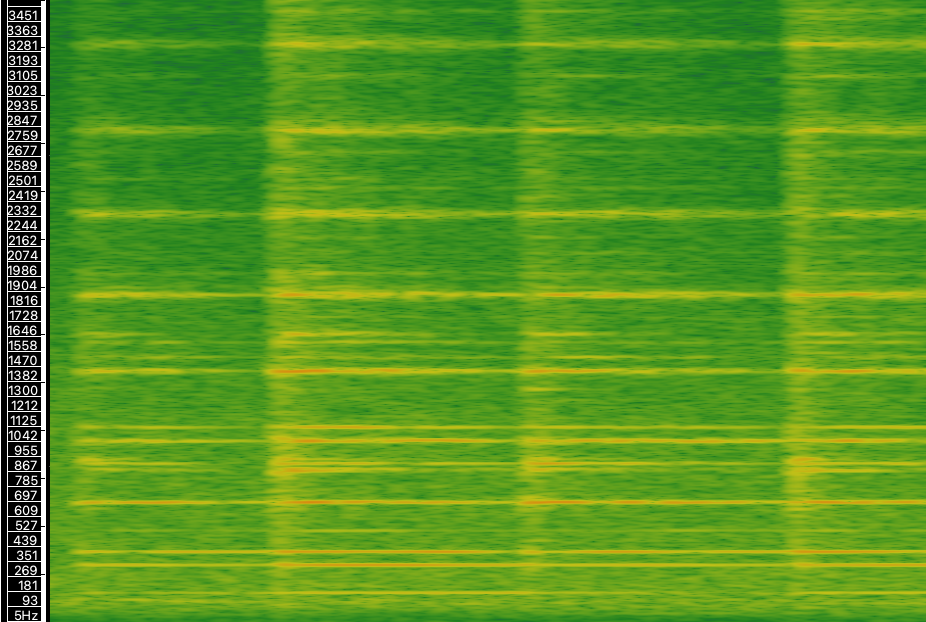
\includegraphics[scale=0.15]{cloche_saint-ed_sonnogram}
    }
    \subfigure{
        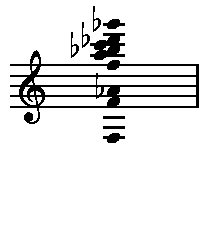
\includegraphics[scale=1]{cloche_analyse}
    }
    \caption{The spectrogram of the four tolls of the low F that opens the recording used for the first movement, and an analysis in western notation on the right.}
    \label{fig:cloche_analyse}
\end{figure}

The use of the word \textit{fugace} in the poetic fragment strongly suggests the traditional form of the fugue, and in this movement, I make use of the chromatic melody described above to construct a fugal exposition in five voices.

\subsection{Form and compositional process}

In the construction of the fifth movement, I was considering two strikingly varied approaches, each representing a strong poetic proposition. 
On the one hand, the slow, ambient texture of the spectral interpolation, and on the other, the integration of the fugue. 
It is not immediately obvious that these two are compatible.
The strong motivic independence that is characteristic of the fugue is not straightforward in a more static framework.
After exploring several ways of merging the two, I settled on having them as fairly discrete units, with the evolutive section coming first, and the fugue section second. 
Typically, a fugal exposition would come at the beginning, but I like the delightful strangeness of finishing the piece with an exposition. 
Furthermore, this subversion of traditional expectations seemed an appropriate choice for the wandering souls of Rilke's poetry, moving forwards while looking backwards. 

\customincludeexamples[width=\textwidth]{5e_2}{ex:5e_2}{The opening to the evolutive section using stop interpolation that was transcribed from an improvisation (mm. 1-11).}

The movement begins with the chromatic melody, entering precisely with the final tick of the recording concluding the fourth movement. The twelfth trigger is then cued, which serves two roles: beginning the stop interpolation (with a delay of several seconds to ensure that the first chord is a Bourdon sound), and triggering another recording, which begins with about 45 seconds of silence for a delayed entry. 
The evolving section itself is a transcription of an early improvisation while testing dissonant clusters with the stop interpolation patch (see \cref{ex:5e_2}.
It begins with the notes D, E\fl, and B\fl, which coincidentally mirrors the notes that I hear in the sound of the fridge of la salle Morin.
The texture then becomes more and more dense, introducing the pedal before thinning and settling on a harmony suggesting E\fl major 6/9. 

By this point, the recording has begun to be audible. 
This sound file is itself a recording of stop interpolation, taken in the church, and was created to serve both as a bridge between the evolutive and fugal sections, as well as to accompany my exit from the organ at the end of the movement. 
The harmonic choice was difficult, because it needed to both sound like the continuation of the evolving section, while appropriately accompanying the fugal section, and not covering it. 
My solution to this problem was to use higher pitches, so that it did not interfere with the other notes of the fugue (especially the bassline), instead acting more as an integrated spectral component to the sound mass. 
I selected pitches from the end of the evolutive section, while avoiding notes that would be too much in conflict with the F minor/C minor orientation of the fugal section.

\customincludeexamples[width=\textwidth]{5e_3}{ex:5e_3}{The end of the evolutive section and opening of the fugue exposition (mm. 12-22).}

The recording continues to play in the background while the fugal section begins with the bright sound of the Cornet (m. 10, \cref{ex:5e_3}). 
I often use this stop to introduce the psalm melody during masses, and to me, it evokes thick incense-filled air. 
Several voices enter the fray and eventually the Cornet is dimmed with the closing of the Récit's expressive box, while the Positif's box is opened, giving more emphasis to the melodie stop (mm. 28-29, \cref{ex:5e_4}). 
This is a technique that I learned from composer and organist Matthew Lane, and represents the closest analogue version of spectral morphing that I can think of with the pipe organ. 
\customincludeexamples[width=\textwidth]{5e_4}{ex:5e_4}{The first appearance of analogue spectral morphing through alternating expressive pedals (mm. 28-32).}

The fugue continues to build, until a five voice texture arrives at a climax (mm.~46-49). The lamentation theme is used in stretto as a coda, before suddenly backing off to a small cluster based around F minor in measure 50.
At this moment, there is a short improvisational section, where rather than improvising notes, the same chord is held while the adding and removal of stops is improvised.
Meanwhile, the expressive pedals are continuously alternated (see \cref{ex:5e_5}). After about thirty seconds of this, the performer stops, leaving the organ while holding a flashlight at chest level and slowly crossing the organ loft and out of sight of the audience. Ideally if this is timed correctly, the recording continues to play, now with lower frequencies introduced, while the player performs their exit.

\customincludeexamples[width=\textwidth]{5e_5}{ex:5e_5}{This movement ends with aleatoric stop selection while alternating expressive pedals (mm. 49-50).}

\section{6\textsuperscript{e} élégie\footnote{24:57--27:18 in elegies\_video.mp4}}

\epigraph{\textit{Figuier, depuis longtemps déjà ce m'est un signe que presque entièrement tu te dérobes à la gloire des fleurs...}}{Rilke, \textit{Les Élégies de Duino}\protect\footnotemark}

\footcitetext[57]{rilke_egies_1986}

\subsection{Narrative context}

To me, this elegy is the crux of Rilke's texts, and the key narrative moment of the piece.
It is like the voice of God acknowledging that the subject is not living up to their fullest potential---that they are shrinking before the greatness of their task.
It is the point in the story where the protagonist must face his mortality, questioning the possibility of continuing, feeling crushed under the weight of burden, as a small fragile child.
For this movement I wanted to make use of what I call the `dissociated Bourdon'.
In this mutation, the harmonic content and the transient noise content (marking the attacks of notes), are treated independently, where the noise sounds on every note onset, but the harmonic content only every sixth onset.
This creates an effect which is haunting and fragile, with fragmented bursts of sound heard interspersed with soft clicking.
Interestingly, without the intermittent removal of the harmonic content, there would have been a fuller contrapuntal message, but it is truncated, hidden, and lost to time.
This is a metaphor for the fig tree, hiding itself and dissociating from its truer form.
In this movement, the performer is completely out of view of the audience, further dissociating the sound from the physical source.

\subsection{Materials and techniques}

The idea for the dissociated Bourdon came as a result of an error of polyphony management when designing OrganLab.
The issue was that my sound was separated into six channels, and instead of triggering each channel on each note event, the code was cycling through the channels, and putting all the harmonic content on the first step.~
The noise content was not subject to this polyphony issue and came through on each step, creating an intriguing texture, largely rhythmic, and punctuated with bursts of organ sound.
I solved the problem, but I was captivated by the result of this `happy error'.
I kept this broken patch set aside, later testing it in the church and recording several improvisations with this effect.
An updated version of this mutation is shown below in \Cref{fig:dissocie}.

\begin{figure}[H]
\begin{lstlisting}[language=Python]
dissCount = 0
def dissocie(x):
    global dissCount
    print(x)
    if x != 0:
        dissCount += 1
        print(dissCount)
        if dissCount > 1:
            stop1.setMul([0, 0, 0, 0, 0, 0, 0, 0, 0, 0, 0, 0, 0, 0, 0, 0, 0, 0, 0, 0])
            print("set0")
        elif dissCount == 1 :
            stop1.setMul([1, 0.01, 0.1, 0.01, 0.07, 0, 0.02, 0, 0.01, 0, 0.003, 0,
	    0.003, 0, 0.001, 0, 0.001, 0, 0.001, 0])
            print("setnon0")
    if dissCount == 4:
        dissCount = 0
\end{lstlisting}
\caption{The function dissocie mutes the harmonic content of the organ synthesis every five notes. For the other four attacks, only the noise of the transient and the air is heard.}
\label{fig:dissocie}
\end{figure}

For poetic and practical reasons, this dissociated Bourdon patch is not played live.
Instead, one of the recorded improvisations described above is used.
I instinctively reached for a pan\=/tonal palette during this improvisation, which seems to adequately represent a sort of pathetic nature.
It is centered in F minor, referring again to the minor triad contained in the harmonics of the spectral analysis of the low F of the carillon of l'église Saint-Édouard.
Structurally, the arrival of the tonality in F minor at the point of great doubt feels thematically consistent.

\subsection{Form and compositional process}

This is the shortest of all the movements, taking just over two minutes. It begins with the performer(s) `offstage', ideally hidden in a room. In my case, there is a door leading into the loft of the chapel of l'église Saint-Édouard which I was able to access. 
From here, just after the ambient recording from the fifth movement fugue ends, the performer sings “Figuier” with an inversion of the principal melody that is truncated to the first few notes (see \cref{ex:6e_1}). 
This single word is repeated five times, and upon each utterance, the closed door of this room is slowly opened, mimicking the opening of the \textit{jalousies} of an organ enclosure.
After this disembodied voice is heard from afar, the recording of the dissociated Bourdon enters.

\customincludeexamples[width=\textwidth]{6e_1}{ex:6e_1}{The “Sixth Elegy” begins with a plaintive cry from out of view, followed by a short and fragile composition heard from the back of the church (p.~15, sys.~2).}

\subsection{Theatrical and spatial elements}

I underline the narrative importance of this movement with a prominent theatrical element.
Having the performer out of the view of the audience establishes a theme of alienation and disembodiment.
Furthermore, the non-live aspect of the dissociated bourdon recording presents an intriguing dynamic\footnote{This recording is unlike others in that it is fundamentally instrumental}. 
On one hand, something is undeniably lost.
The immediacy of music performed in real\=/time is replaced with the automaton.
However, from a narrative perspective, the recording is even better.
The timbral dissociation is linked with the physical disembodiment of the performer and their sound.
Since the performer is in another room, the audience is left to wonder what the source of this sound is putting the role of presence and physicality in music-making into question..
Is the performer playing it from somewhere?
Is it pre-recorded?

At the same time, to increase the poignancy of the theme of alienation, I relocate not only the performer, but also the sound itself.
Instead of using the same speakers that have been used thus far (speakers one, two, three, and four in \cref{fig:mapping}), a separate sound system located in the second balcony in the back of the church (speaker five) where the organ originally stood sounds the dissociated Bourdon recording.
At the same time, a flashlight with a cold light is illuminated in this same space.
From a technical standpoint, this in theory could be controlled with software, LEDs, and a cabled connection, but it was more practical to ask a friend to stay in the balcony with a flashlight during the performance, awaiting an auditory cue (the final incantation of `Figuier').
The helper not only turns on the light, but triggers the recording, ensuring that the two are reasonably synchronous.
Seeing as the light is behind the audience, it is very possible that this effect is not noticed by certain audience members.
At the same time I like the idea of a hidden element that is only apparent to some.
This simple visual elaboration signifies on the one hand, fragile, yet constant spiritual presence of our protagonist, symbolized as a fig tree, and simultaneously represents the phantom of the organ in its original home, now vacant.
It also invokes the separation of the traditional physical performer and the mechanized, automated version---the ghost in the machine.

\section{7\textsuperscript{e} élégie\footnote{27:58--35:35 in elegies\_video.mp4}}

\epigraph{\textit{Non, plus d’imploration, voix maintenant mûrie, plus de clameur...}}{Rilke, \textit{Les Élégies de Duino}\protect\footnotemark}

\footcitetext[63]{rilke_egies_1986}

\subsection{Narrative context}

Following the fragile unsurety of the sixth movement, the seventh represents a call to action, as if our protagonist, half awake from their frozen dream, summons themself with an urgent plea. 
It isn’t clear whether this plea is from within, or from some external source, but it seems to imply some impending event. 
To me, this symbolizes a calm before the storm, a rising tension before the final climax. 

I explore this tension is several ways. 
Firstly, the sonic elements are quiet and eerie, prominently featuring a low drone. 
Combined with the total darkness that the audience now finds themselves in, these elements establish a tone of apprehension.
Secondly, the performer is still not present at the instrument, but makes several brief appearances elsewhere in the church, adding to a sense of unease. 
The obscured identity of the figure suggests a multiplicity of our protagonist, none of whom are fully embodied---only existing for mere moments like transient phantoms.

In this movement, both the fourth and fifth stations of \textit{le chemin} are evoked simultaneously, indicating a overlapping of place and time. 
The protagonist is at once in the underbelly of the furnace room, and in the church itself. 
Interestingly, this is the only movement in the piece to not have a vocalized component, adding to the theme of disembodiment explored in the sixth and seventh movements.
It is as if our protagonist is muted, emphasizing an interiorized experience.
This means that the selected poetic fragment is unused, but it nonetheless informs the narrative framework. 

In several ways, the last four movements are merged into one. 
There is no break in between, unlike the preceding movements, with a series of recordings sounding continuously until the end. 
The coupling of Rilke's elegies to the corresponding movements is also more abstract, with a blending of formal elements that parallels the spiritual awakening in Rilke’s poetry. 
Attempts will be made throughout these last sections to carefully clarify where these overlapping elements are in play.

\subsection{Materials and techniques}

The techniques used here are different than all the preceding movements. 
Instead of being based on synthesis, this movement delves into the electroacoustic domain, layering and transforming various sound sources throughout its roughly seven minute duration. 
Sampling of bells, in particular, provide an intriguing proposition. 
The carillon is the heaviest instrument in the world, and as such, a pitch bend would be unthinkable. 
Similar to the pipe organ's fixed pipes, altering the pitch of a bell would involve changing its size in real\=/time. 
Unlike the voice, which is extremely malleable and versatile, the carillon is rooted and immutable. 
The application of pitch envelopes then gives the carillon a more organic quality, as if this massive, suspended titan, is given liquid form, called down from the heavens to express itself in a vocal way.

Another key element is a sample of the fire alarms of the church, which sounded one day while I was recording and experimenting with dissonant clusters. 
The sound surprised me, and I wasn’t sure what it represented. 
I considered stopping to investigate, but decided to continue. 
During the movement I employ both the alarm by itself, as well as the sounds of this organ improvisation.
The alarm and the thick clusters of organ chords create a sense of dramatic tension and impending, appropriate with the urgency of the poetic fragment. 

An additional theme developed in this movement is the sound of footsteps, recorded with my Zoom H4N recorder. 
These footsteps were recorded during a session where I was attempting to create a near-infinite reverb, trying different microphones and decay intervals, with most feedback quickly becoming out of control. 
One, however, seemingly a product of the space itself, established a stasis, neither growing nor diminishing and remaining in a constant periodic pulsation. 
I had already planned to record the sound of running towards the microphone later in the day, but I was so moved by the eerie tension of this sound, that I decided to try recording the footsteps directly overtop of it. 
The intention was to accent a sense of urgency, playing off the footsteps motive that has been heard throughout \textit{le chemin}, yet now decoupling the subject and the sound source, creating an almost cinematic effect where the listener is no longer following over the shoulder of the protagonist, but is suddenly viewing the protagonist, or some person or animal, which is running towards them. 
In the composition of this movement, I make use of both the footsteps and the feedback drone.

\subsection{Form and compositional process}

After the sixth movement, the small amount of light in the west gallery provided by the flashlight is extinguished, leaving the audience in dark silence. 
Out of this silence, an electroacoustic piece begins, cued with OSC (see \cref{ex:7e_1}). 
We first hear the sound of a match being struck, with a soft, dissonant drone heard in the background (the feedback loop described above). 
Then, a heavy sliding metal door is heard opening
The match serves a dual role here.
On the one hand, it signifies, along with the feedback sounds, the entry into the church in the fifth station of \textit{le chemin}, evoking the religious \textit{lampions} that are lit in prayer.
On the other, it symbolizes the darkness of both the audience and our protagonist, and the need of light.
The opening of the metal door represents the fourth station, a descent into the furnace room.
I imagine the protagonist opening this match to light their way before entering.

From 28:15 to 28:52 we hear the clicking of the furnace, footsteps, and the jangling of keys, which swells twice only to cut out abruptly each time, leaving only the soft feedback drone. 
The abruptness of these silences is not present in previous movements, now highlighting the surreal nature of the recording, making clearer than ever that it represents a time and place that is other than the current moment. 
It further signals the darkness of the moment, creating the sensation of glimpses of light illuminating the space for a brief time only to be extinguished. 

Then, samples of the church bells enter (28:58), placed in a low register with pitch and dynamic envelopes. 
This is punctuated with two moments where Michael Norris's Spectral Blur plugin, which was applied very slightly in the opening bed track, is applied in a more extreme way, creating an icy, crystalline texture---once at 29:38, and again at 30:03. 
The fire alarm gradually emerges by 30:59, becoming more and more present, and over this texture, the organ recording is introduced (31:40). 
By about 32:40, this recording recedes into the background, while the bell sounds return to the forefront, this time less processed, and placed in a middle register when they sound less menacing and more haunting. 
At the same time, fragments from the sixth movement's dissociated Bourdon are heard, transposed higher and sped up.

This is followed by two swells of pink noise, first from 33:08 to 33:24, and then from 33:32 to 33:55.
Pink noise is what I use in OrganLab to simulate the ambient noise of the wind chest, and these swells are intended to evoke these windchests, which are normally a constant volume, threatening to lose control.
At the same time, they harken back to the recording of the July 2023 storms from the opening of the first movement and surges sweeps of wind.

The second swell represents the climax of this movement, and perhaps of \textit{Élégies} as whole.
Up until this point, the electroacoustic track is played from the second and third speakers, located in front of the audience on either side of the choir.
During the swell, however, the sound is sent to the fourth speaker in the tribune opposite the organ loft.
It is then passed gradually to speaker one, next to the organ.
This effect was inspired by a moment while working when a plane passed overhead, and the sound seemed to sweep the church, not unlike the rays of light that often pass through the church, leaving a shadow in its wake. 
This sonic shadow play, once arriving completely in the organ loft, suddenly cuts out entirely, while an intensified version of the feedback drone, transposed down an octave, is suddenly sent to speakers one through four, surrounding the listener (33:55).
This subtle though arresting effect is difficult to capture in the stereo recordings that accompany this thesis.
Its deep resonance creates a sense of immersion and envelopment that is unique at this point in the piece. 
Previously, the only time when these four speakers are used is in the opening sound recording, though here, the sound was not simultaneous. 
Furthermore, after the slow, evolutive nature of this and many prior movements, it is very satisfying to have a gesture that is sudden, clear, and decisive. 

From this moment on, the low throbbing drone continues on uninterrupted, while the sounds of urgent footsteps enter several times---seemingly encircling the audience---with the fire alarm faintly present. 
By about 35:45, the audio enters into a loop of about one and a half minutes, in which the throbbing continues, the fire alarm fades in and out of perception, and some faint footsteps and sounds of keys are heard.  
This loop, as in the first movement allowing the performer to take their time making their way back and establishing themself at the organ console.

\customincludeexamples[width=\textwidth]{7e_1}{ex:7e_1}{The “Seventh Elegy” is summarized in one system (p.~15, sys.~3).}

\subsection{Theatrical and spatial elements}

During this movement, the performer remains offstage. 
The intention with this decision is to continue the sense of disembodiment established in the sixth movement. 
Whereas the musical element in the sixth could imaginably be played on a single instrument, due to its minimal, soloistic nature, the seventh movement is so densely layered that it is clearly an electroacoustic piece. 
This has the effect of dissolving even further the relationship between the sound source and the physicality of the performer. 
The audience is no longer imagining the musician’s hands, but is now lost, in a dreamlike way, in visions, symbols, and memories. 

This mirror’s the effect of the footsteps described in the previous section. 
Just as the sound of the footsteps approaching the microphone creates a sense of embodied experience, rather than simple voyeurism, the aural landscape is transformed from one that is voyeuristic and observational, to one that is more interiorized and subjective. 
During this movement, rather than resting off stage as in the sixth, I traverse the space of the church, appearing briefly several times, first in the north entry of the choir, and then in the south transept tribune opposite the organ loft. 
During both of these apparitions, I appear, remain completely immobile for a short time, illuminated only by a flashlight held at my chest and pointed upwards, and then disappear.

From a practical perspective, I realized that in order to appear in the balcony opposite the organ, I couldn't do so without leaving the church. 
The simplest solution would have been to simply walk directly through the line of sight of the audience and mount the stairwell, but I wanted to create a sense of magic and mystery, seeming to appear out of nowhere. 
In order to make this work, I exit the church through the door of the Chartier hall immediately after my first apparition. 
Running quickly around the building, I enter the church from the entrance on Beaubien, climbing the stairs and making my appearance while deeply out of breath. 
I then descend the stairs to traverse the same route in the opposite direction.
These apparitions are subtle, and will not be noticed by every audience member, but like the light in the west gallery in the previous movement, this provides a hidden aspect to the piece, providing a potential private experience in a shared setting. 

\begin{figure}[h]
    \centering
    \subfigure{
        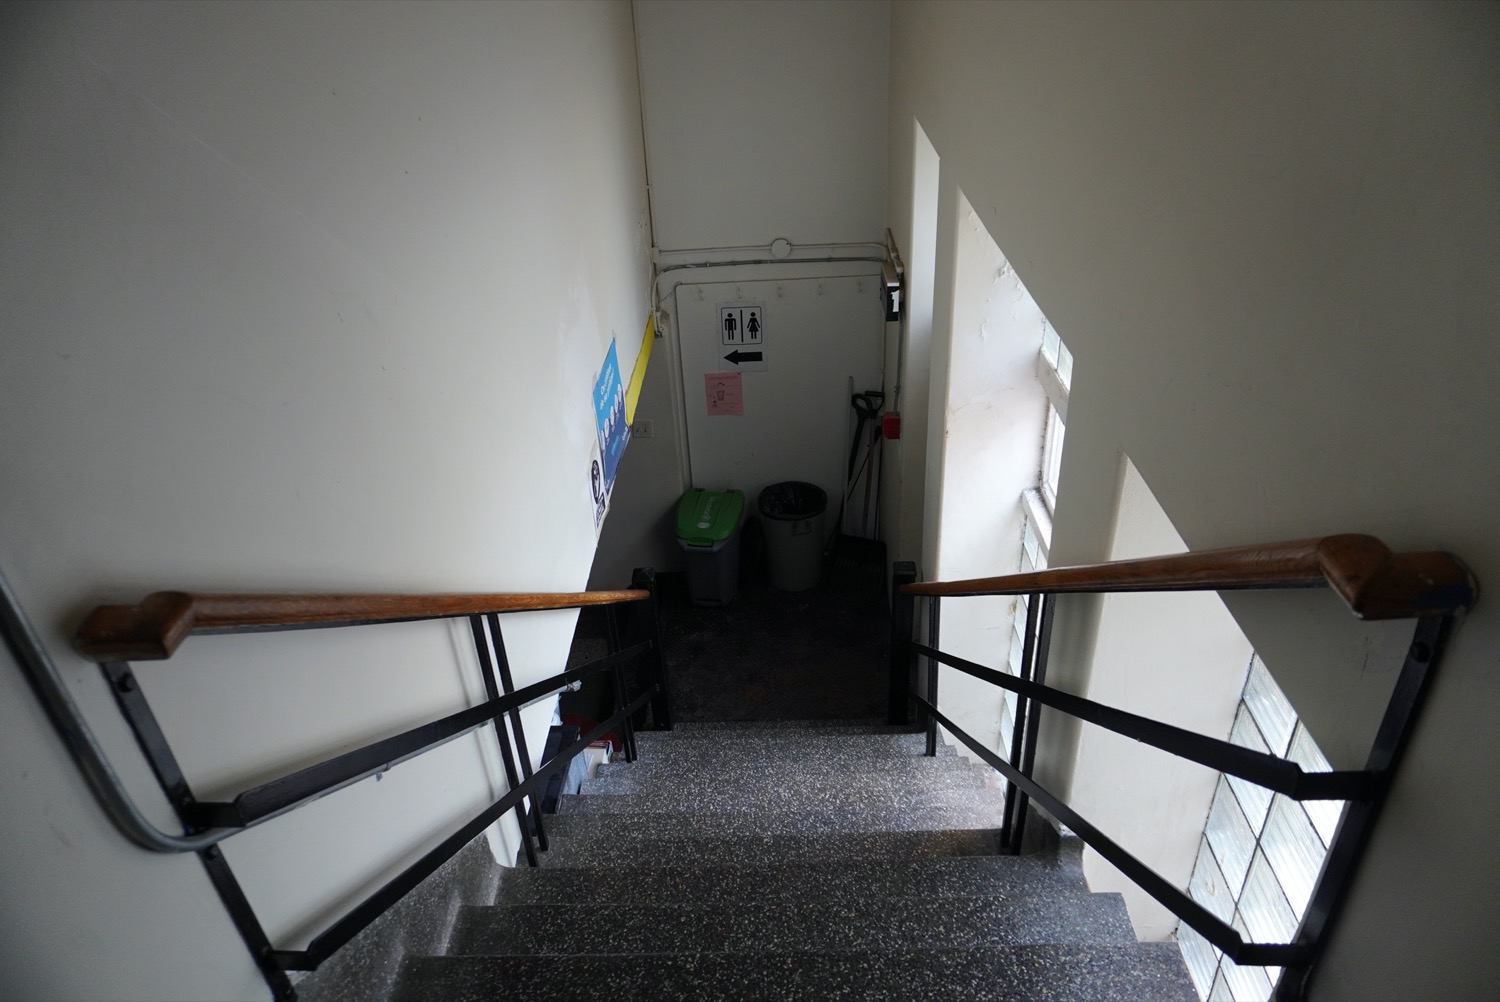
\includegraphics[scale=0.15]{DSC00160.JPG}
    }
    \subfigure{
        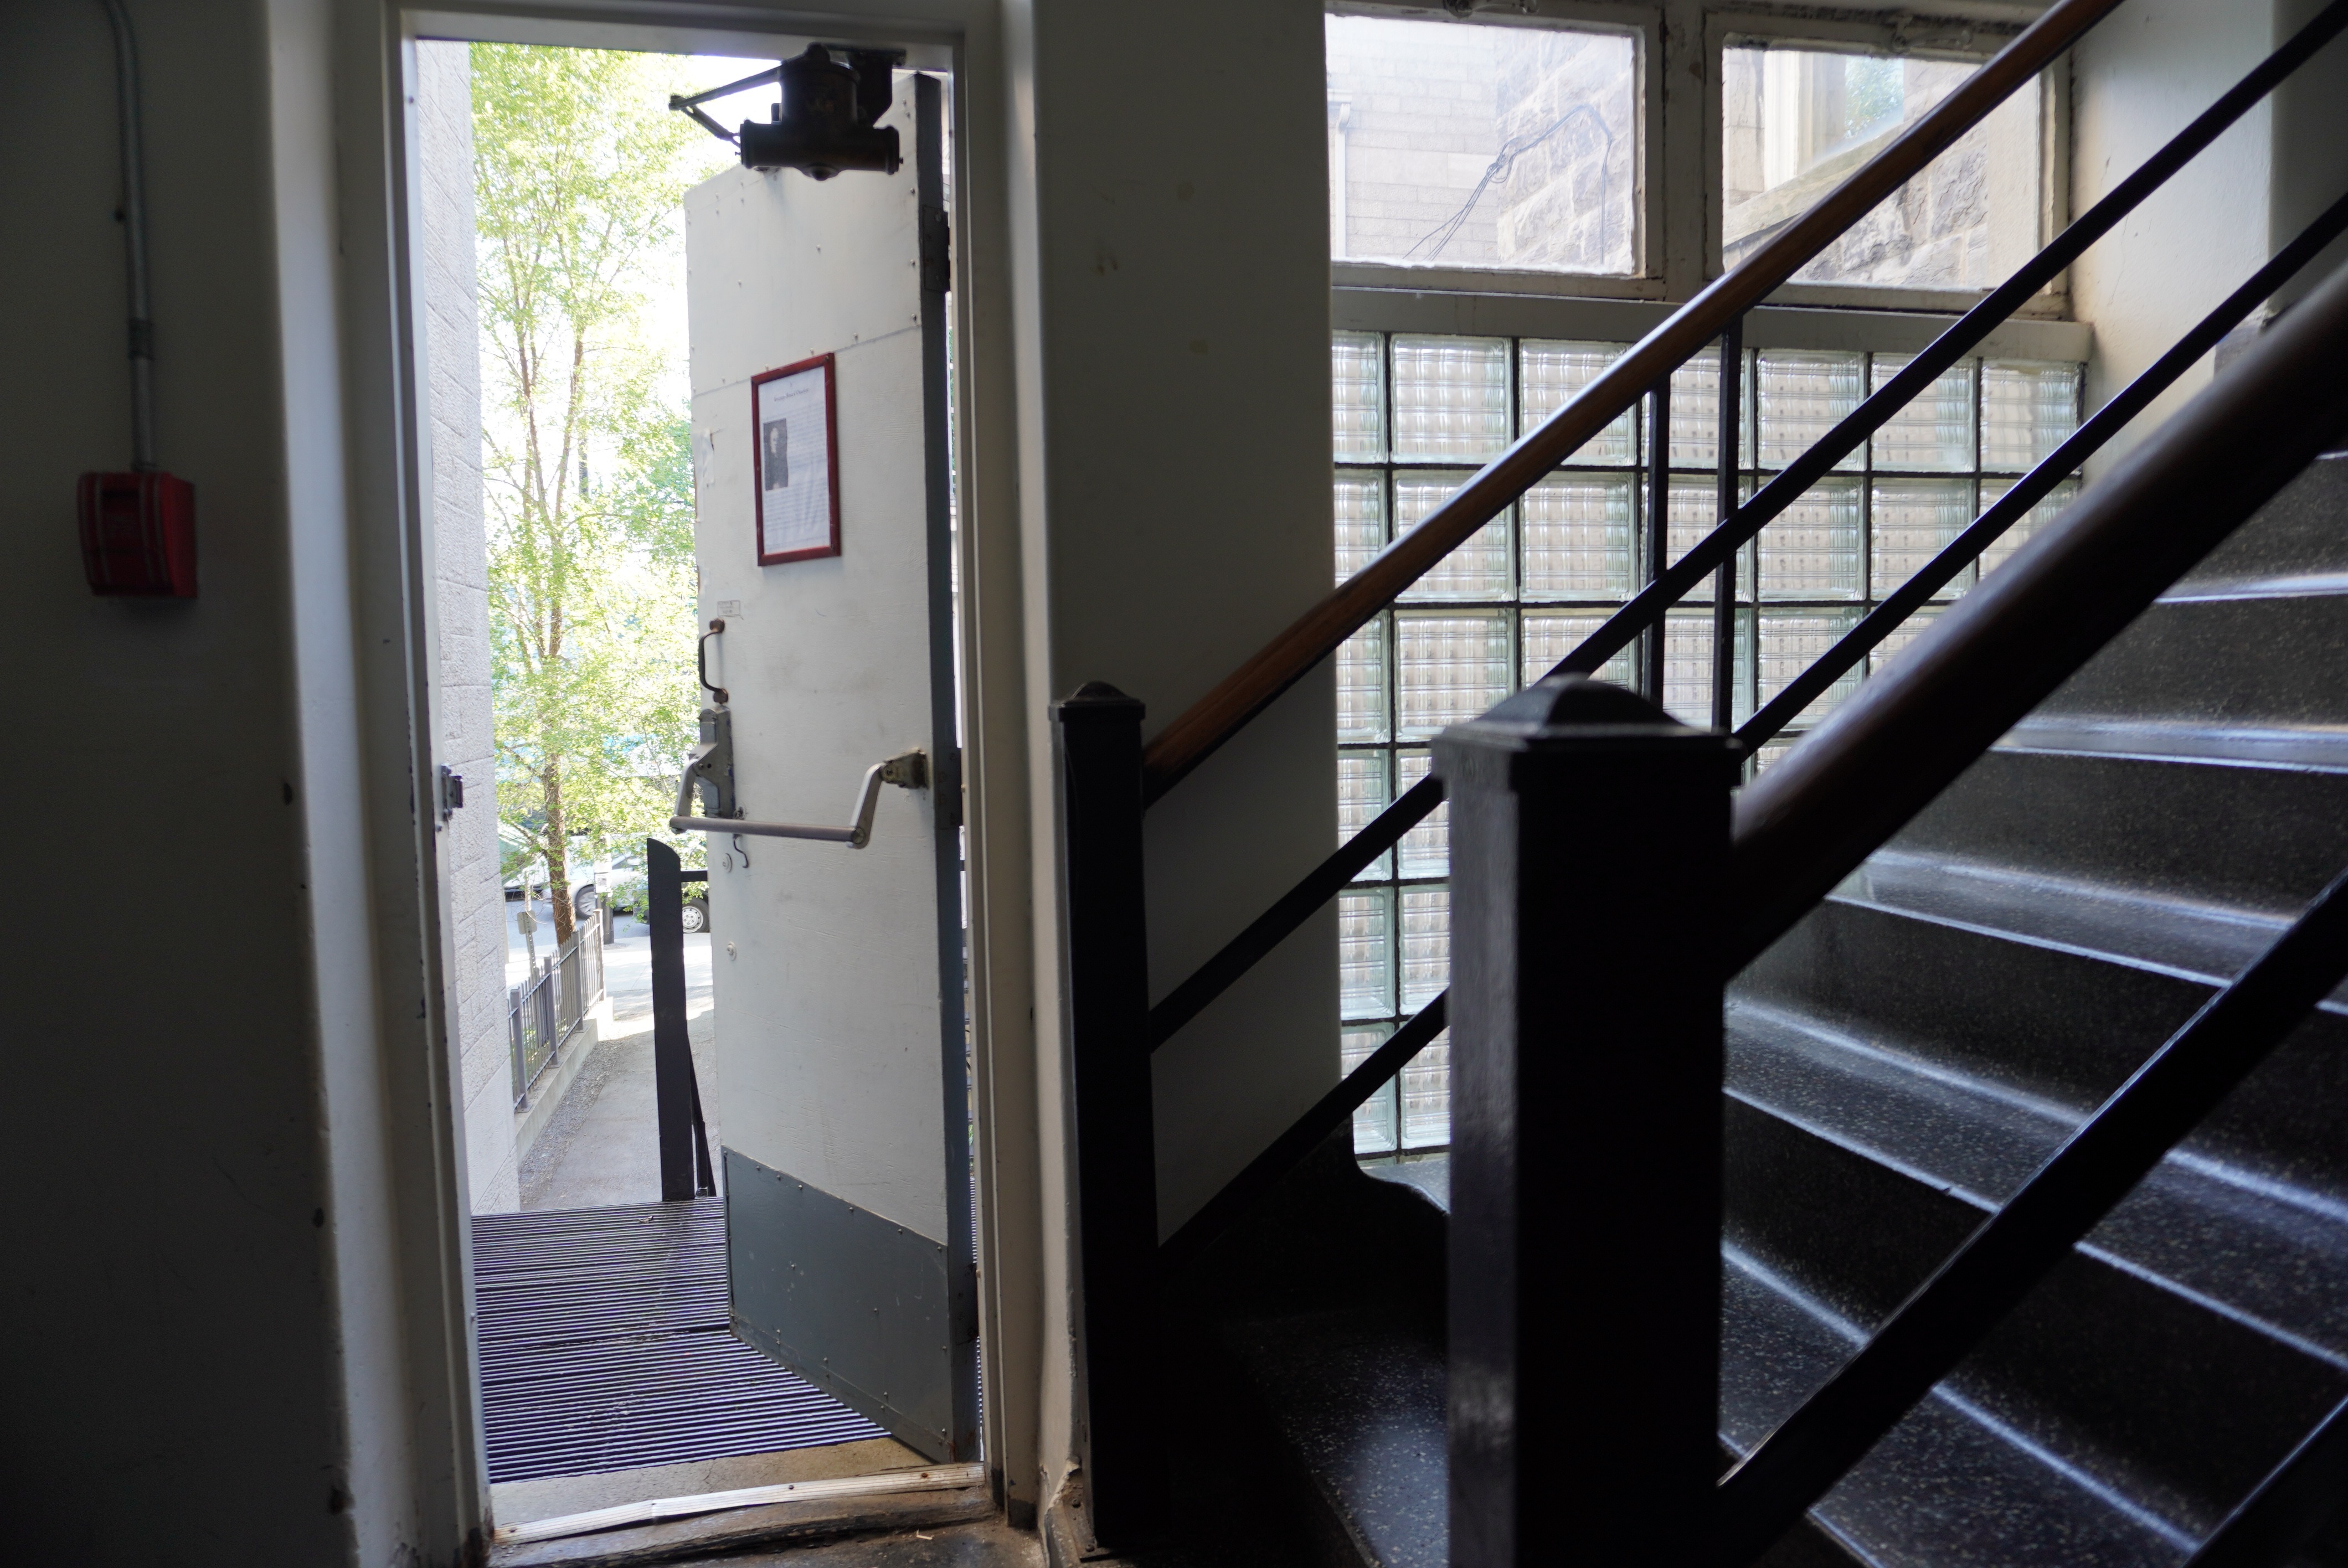
\includegraphics[scale=0.15]{DSC00171.JPG}
    }
    \caption{The door leading from the Sacristie to la salle Chartier on the left, and the door leading to the north exit on the right.}
    \label{fig:chartier}
\end{figure}

The strangeness of these appearances, and the disconnect between the sonic experience and the human form, heighten the sense of disembodiment and tension, paralleling the theme of hauntology and acting as a phantom presence. 
Due to the relatively dark conditions, my identity remains unclear, leading audience members to question whether it is indeed me or someone else, as if the phantom is duplicated, or transported throughout the space.

Once the electroacoustic track arrives at the looping point, the performer reenters the view of the audience. 
Although the score marks this as the beginning of the eighth movement, I see it as a liminal space between the seventh and eighth movements---a threshold where the boundaries between the two begin to blur.

\section{8\textsuperscript{e} élégie\footnote{35:35--40:23 in elegies\_video.mp4}}

\epigraph{\textit{A plein regards, la créature voit dans l’Ouvert.}}{Rilke, \textit{Les Élégies de Duino}\protect\footnotemark}

\footcitetext[75]{rilke_egies_1986}

\subsection{Narrative context}

The “Eighth Elegy” represents a pivotal moment in \textit{Élégies}, marking a shift from the helplessness and impotence described in the sixth movement to a powerful sense of awakening and transformation. 
The text, “À plein regards, la créature voit dans l’Ouvert”, suggests the emergence of something nascent---a being still in the process of becoming. 
I imagine Rilke's creature gradually taking shape, forged from raw potential into a yet unrealized form, as if being called into existence, rather than simply roused from slumber.

This movement occurs after the fully electroacoustic seventh movement, at which point the audience has not seen the performer for about ten minutes, save for a few apparitions away from the instrument, and begins with the organist approaching the organ, carrying a flashlight pointed upwards. 

\subsection{Materials and techniques}

This movement is the first to make use of live effects, employing both delay and distortion. 
The delay is directed towards the tribune opposite the organ loft, creating a spatio\=/temporal effect that spans several seconds. 
This effect, as described in chapter three, signifies a broader echo through history, engaging in dialogue with generations past. 

Distortion is applied both in combination with the delay, and by itself.
With the echo, distortion aids to further distinguish the sound source from its affected version.
Used on its own, distortion acts as a thickener, filling the spectral space and creating an aggressive tone reminiscent of the electric guitar.

Another element is the use of a sampler based on feedback from the church space itself. 
This feedback was recorded in complete silence, without any input from the organ or voice. 
By gradually raising the gain on a dynamic microphone, the natural room resonance and the noise floor of the microphone were amplified, producing a rich, inharmonic sound. 
Sampling this feedback allows the performer to play the resonance of the space in an instrumental fashion, adding an intriguing dimension that is integrally connected to the church acoustics. 

Lastly, this movement introduces clear amplification of the voice with live effects. In previous movements, the voice is amplified only slightly, so as to make the text audible while maintaining an acoustic quality.
Here, however, the level of amplification in increased, while a vocoder is applied using the bell recording from the first movement as a carrier, merging the maleable human voice with the immutable carillon.

\subsection{Form and compositional process}

Once arriving at the organ, the performer makes the necessary registral changes in preparation for the final movements. 
They then initiate the 14\textsuperscript{th} trigger, which activates a 3.5\=/second delay and distortion on the organ sound. 
The organist then enters with soft chords played on the Récit(p.~16, sys.~1, \cref{ex:8e_1}), echoing the parallel stack of fifths heard at the end of the first movement. 
However, after the third iteration, the chords diverge from the original fifths, transitioning into a series of Major 7 and Minor 7 chords, mainly in drop 2/4 voicings. 

\customincludeexamples[width=\textwidth]{8e_1}{ex:8e_1}{Soft chords harking back to the end of the intial movement mark the performer's return to the instrument (p.~16, sys.~1).}

As the volume and intensity of the chords increase, the music shifts from the Récit to the Positif (with Récit coupled), and finally to the Grand Orgue (with both Récit and Positif coupled). 
The distortion in the echoes becomes more pronounced, and feedback loops begin to form, heightening the sense of chaos. 
At the peak of this intensity, the performer presses the 15\textsuperscript{th} trigger, which turns off the delay while allowing existing echoes to naturally decay. 
Following this, the pedals enter with an imposing sound (p.~16, m.~1, see \cref{ex:8e_2}), combining the 32' and 16' flutes with a bright plein orgue registration from the Grand Orgue. 
The resulting sound has an aggressive edge that is complemented by the distortion. 
Coupled with a rumbling undertone from the lower registers, this creates a powerful, resonant presence that preempts the creature’s emergence.

After six measures of solo pedal, the performer’s hands enter on the Grand Orgue with dissonant chords (m.~7), each preceded by a rapid triplet figuration, further energizing the distortion. 
The performer then switches to the MIDI keyboard, playing held notes of the sampled feedback (m.~13). 
These sampled notes are played between sections of the Grand Orgue, serving as moments of mysterious reflection amid the bursts of intense organ sound.
After the final section of sampled feedback, where the tension peaks with a dissonant C4 against a D4, the organ suddenly drops out, creating a dramatic silence (see \cref{ex:8e_3}). 

\customincludeexamples[width=\textwidth]{8e_2}{ex:8e_2}{The entry of the pedal, with coupled plein orgue. At the end of the system is the first entrance of sampled feedback (mm. 1-15).}

Simultaneously, the performer triggers the 15\textsuperscript{th} cue, which silences the low rumble of the drone that has persisted since the end of the “Seventh Elegy”. 
At this moment, the sound of a match being struck is heard for the second time, signifying illumination in the enduring darkness, as if the form of our creature is being revealed. 
The crackling match is followed by a rolling, rhythmic sound, gradually growing louder as it moves from the fourth speaker to the first, echoing the pink noise effect of the “Seventh Elegy”.

As the rolling rhythm reaches a dynamic peak, a loud crack of thunder is heard nearby, marking a dramatic shift. 
A driving beat inspired by UK dubstep rhythms enters, woven from samples of keys, footsteps, and taps and strikes of the pews recorded in l'église Saint-Édouard (\cref{ex:8e_3}). 
This rhythm creates the sense that the church itself is participating in an ecstatic dance, introducing a distinctly pop\=/influenced sound into the piece for the first time. 
Simultaneously, the voice enters with a variation on the falling third motive from the opening vocal gesture, sung in subharmonics to create an eerie, non-human sound. 
During this passage, the vocoder is applied gradually, referencing the bell transformation heard in the “Third Elegy”, but now realized in an embodied, rather than simulated vocal context.

\customincludeexamples[width=\textwidth]{8e_3}{ex:8e_3}{The voice singing subharmonics against the bed track as well as the entry of the bassline over the beat (mm. 31-38).}

\section{9\textsuperscript{e} élégie\footnote{40:23--45:04 in elegies\_video.mp4}}

\epigraph{\textit{Pourquoi, s’il est loisible aussi bien de remplir son délai d’existence en laurier, sombre un peu plus que tous les autres verts, avec ces vaguelettes...}}{Rilke, \textit{Les Élégies de Duino}\protect\footnotemark}

\footcitetext[83]{rilke_egies_1986}

\subsection{Narrative context}

The ninth movement represents a departure from the patterns established in the previous movements of \textit{Élégies}, both in its structure and thematic content. 
It begins with text drawn not from the “Ninth Elegy”, as one might expect, but from the tenth. 
This choice emerged from a deliberate consideration of how to integrate Rilke’s dense and multifaceted final elegy into the musical narrative. 
Musically, the “Tenth Elegy” seemed to demand a reflective, non-vocal resolution, serving as a calm after the storm of the preceding movements. 
To maintain the established pattern of incorporating sung lyrics in each movement, the text of the “Tenth Elegy” is instead woven into the fabric of the ninth.

Unlike the previous movements, which each make use of the opening words of Rilke's poems, the lyrics from the “Tenth Elegy” are taken from from various parts of the “Tenth Elegy”. 
This reconstruction, shown in \Cref{fig:poem}, is a fragmented mosaic, creating a tapestry of incomplete thoughts and potentialities, mirroring the themes of joy, grief, and longing in Rilke’s poetry. 
This movement, like the text it draws from, grapples with the fear that accompanies happiness--the knowledge that it is transient and inevitably fleeting. 
Musically, this movement emerges directly from the eighth, with the beat and bassline that arrive at the end of the previous movement as a link.

\begin{figure}[H]
\begin{verse}
Vienne le jour, enfin sortant.\\ 
La pluie qui vient tomber dans les venelles de la Cité,\\ 
prête à se briser. Mon visage resplendissant, baigné.\\ 
Aux Anges qui l'agréent, des marteaux du cœur.\\
\end{verse}  
	\caption{My reconstruction of poetic fragments from Rilke's “Tenth Elegy”} 
\label{fig:poem}
\end{figure}

\subsection{Materials and techniques}

This movement does not introduce any new techniques, but attempts instead to develop on previous ones.
The melody of lamentation, doubled with the voice, is harmonized with parallel minor 7 chords, transforming it from its original 17\textsuperscript{th}\=/century idiom into a modern, R\&B\=/inspired tone. 
The arch theme is also revisited, this time with the arpeggios in the right hand, while the left hand plays a variation on the lamenting theme, doubled by the voice.
The effects remain the same, with distortion and a vocoder applied to the voice.

\subsection{Form and compositional process}

The “Ninth Elegy” begins as the voice joins the sparse texture of sample based beat against pedal bassline that emerges at the end of the “Eighth Elegy” (\cref{ex:9e_1}). 
The aesthetic of this section is perhaps the closest to a UK dubstep sound, with the throbbing bass, skittering rhythm, and plaintive, repetitive vocal line recalling Burial's “Archangel”. 
The vocal line, opening with “Vienne le jour, enfin sortant”

\customincludeexamples[width=\textwidth]{9e_1}{ex:9e_1}{The entrance of the voice over the sparse texture of pedal bassline and sample-based rhythm (mm. 1-8).}

After the initial section, the vocal line drops out, leaving the bassline and beat to carry the momentum for six measures. 
The R\&B\=/influenced version of the melody of lamentation then enters in A minor  (m. 49, see \cref{ex:9e_2}). 
The three final lines of the poetic reconstruction are sung over three iterations of this melody\footnote{In the April performances, I was still in the process of setting this text, and so the recordings accompanying this thesis use nonsense syllables for this section.}, with the organ accompaniment passing from the Positif to the Grand Orgue with the second, and then moving up an octave while introducing the pedals in the third.

Following these iterations, 17\textsuperscript{th} trigger is initiated, lowering the volume of the beat such that it becomes a distant echo, reminiscent of the familiar groanings and clatterings of the church building, or those of the city itself. 
This shift in dynamics allows the organ to take center stage, presenting a solo variation of the melody of lamentation' in D minor (mm.~53-74, see \cref{ex:9e_2}). 
This variation involves a tonicization of G minor, leading into a descending third, rising second sequence.

\customincludeexamples[width=\textwidth]{9e_2}{ex:9e_2}{The transition from the second vocal melody into the extended solo organ version with the rhythmic loop in the background (mm. 49-58).}

As the beat fades out, the 18\textsuperscript{th} trigger initiates a sound file taken from the same recording used in the opening of the piece but focused on the rain rather than the thunder. 
As shown in \Cref{ex:9e_3}, the melody of lamentation reappears in a simplified form, stretched to two notes per measure and played in the left hand, while an arpeggiated figure is taken by the right. 
This is a direct reference to the fourth movement, though the roles of the hands are now reversed. 
Over this framework, the voice re-enters, singing an incomplete question to the assenting angels: “Pourquoi, s'il est loisible aussi bien de remplir son délai en laurier. Pourquoi s'il est loisible…” (m.~78)
The performer then triggers the 19\textsuperscript{th} cue and engages the tremulants before moving to the final movement. 

\customincludeexamples[width=\textwidth]{9e_3}{ex:9e_3}{The lament melody simplified and quantized to whole notes in the left hand, with the arch theme in the right hand, with voice (mm. 79-81).}

\section{10\textsuperscript{e} élégie\footnote{45:04--49:13 in elegies\_video.mp4}}

\epigraph{\textit{Vienne le jour enfin, sortant de la voyance encolérée, où je chante la gloire et la jubilation aux Anges qui l’agréent. Que des marteaux du cœur au battement très clair aucun ne vienne à faux tomber sur une corde molle, ou encore douteuse ou prête à se briser.}}{Rilke, \textit{Les Élégies de Duino}\protect\footnotemark}

\footcitetext[91]{rilke_egies_1986}

\subsection{Narrative context}

The “Tenth Elegy” stands as a contemplative epilogue, a reflective meditation that diverges from the narrative drama of the previous movements. 
This movement uniquely omits the human voice---an absence which indicates otherness, suggesting that this movement is not participating in the unfolding drama but is instead observing, reflecting, and internalizing the previous events. 
This silence points to the idea that the text of the “Tenth Elegy” is not meant to be embodied or expressed outwardly but is rather an internal, imagined experience.

Rilke’s final elegy grapples with the themes of joy, grief, and the haunting realization that our most profound desires and potentials may remain forever unfulfilled. 
The decision to relegate the text of the “Tenth Elegy” to the ninth movement, where it is fragmented and distorted, introduces a layer of ambiguity. 
This dislocation raises the question of whether the events depicted in the “Ninth Elegy” truly transpired or if they were merely a projection of the protagonist's inner world---a dream of fulfillment that remains just out of reach.

\subsection{Materials and techniques}

This movement is focused around three main elements.
The recording of bells from the first movement is heard in reverse, representing the sixth station in \textit{le chemin}, as well as a montage of the sounds of pigeons combined with a recording of myself coming from the basement of the church and ascending the stairs to the organ loft, representing the seventh  and final station. 
In terms of live effect, an infinite reverb is applied, and a short delay provides a more subtle effect.

\subsection{Form and compositional process}

The “Tenth Elegy” opens with the ethereal sound of reversed bells, initiated by the 18\textsuperscript{th} trigger. 
This is layered with a shimmering plein orgue sound, executed through a two\=/handed tremolo technique with each hand playing the same chord an octave apart (see \cref{ex:10e_1}). 
The combination of tremulants and a 50ms delay adds a fluttering, almost dizzying texture that mirrors the swirling thoughts of reflection and introspection. 
Beneath the active surface, the harmonic progression moves slowly, repeating IV-V-I cadences in F major and Ab major. 
This harmonic ambiguity reflects the coexistence of F major and F minor in the spectral composition of the carillon's low F.

\customincludeexamples[width=\textwidth]{10e_1}{ex:10e_1}{A tremolo between the two hands, with both tremulant motors active, and a slight delay (mm. 1-9).}

\customincludeexamples[width=\textwidth]{10e_2}{ex:10e_2}{A 6/5 5/3 sequence, followed by the last iteration of the initial theme of the piece (mm. 25-32).}

This section ends with a 6--5 sequence, shown in \Cref{ex:10e_2}, followed by a final, reharmonized version of the initial theme first heard in the voice in the first movement. 
The last trigger then turns on a long reverb effect of about sixty seconds which attempts to augment the already significant reverb of the church to something that is essentially frozen in time. 
To represent this timelessness, the notation dissolves into proportional notation (see \cref{ex:10e_3}), and several frozen, falling by step motives are played as the final audio recording is introduced. 
We hear pigeons speaking and fluttering their wings, at first in real-time and gradually slower, which is juxtaposed with the sound of my ascent to the organ loft, mirroring the ascent that begins the piece. 
Because the microphone was placed at the bottom of the stairs to the organ loft, and at the top of the stairs from the basement, my steps are heard approaching, and then moving into the distance. 
On one hand, our protagonist has ascended, like the ascension mentioned in the last passage of Rilke's \textit{Elegies}. 
At the same time, what this ascension represents is unclear.

\customincludeexamples[width=\textwidth]{10e_3}{ex:10e_3}{The final moment of the piece, with a repeated descending motive with frozen reverb against the sound of pigeons and footsteps (p.~27, sys.~2).}

\chapter*{Conclusion}

In this text, we have gradually elucidated a personal approach to pipe organ augmentation.
In chapter one we established the context and diverse problem space of instrument augmentation broadly, beginning with the foundational work of Tod Machover, then Cléo Palacio-Quintin's hyper-flûte and McPherson's magnetic resonator piano, and ending with several varied approaches for pipe organ augmentation.

In the second chapter, we investigated my personal approach to extending the expressive potential of the organ of l'église Saint-Édouard, and the process of developing a tri-modal augmented interface including synthesis, live effects, and fixed media.

Chapter three dealt with my creative framework, both in addressing the hyper-instrument outlined in chapter two, as well as the formation of an extended practice that addresses the pipe organ not only as an instrument, but as an architecture, emphasizing the sacred space in which it dwells through multichannel sound diffusion, references to various spaces from throughout the church spaces, as well as the carillon through audio recordings, and the inclusion of the voice, which as a primordial, embodied expressive instrument, provides an intuitive counterpoint to the pipe organ's technological, abstracted paradigm. 

Then, in the fourth and final chapter, we analyzed the piece \textit{Élégies} in its entirety, moving movement by movement while attempting to grasp the important elements in its construction, including the poetic interpretation of Rilke's \textit{Duino Élégies}, the musical material employed and its development over the course of the piece, the various dramaturgic aspects that go beyond purely instrumental writing and add an important narrative dimension to the piece, and the composition of these elements into a cohesive, communicative structure. 

Now that \textit{Élégies} exists as a proof of concept, the question remains: “where to go from here?”.
As McPherson and Kim note, contemporary music and musical interfaces face the issue of perennity, with many projects serving the means of a given context, only to fall to disuse and abandon. 

This is not necessarily a negative thing.
Temporality is the way of life, and there is beauty in a creation that fulfills a function for a limited time.
At the same time, there is something to be said for a project that perseveres, not as a monolith, but as a breathing organism---taking on new forms and adapting to changing needs and perspectives.   

I have several ideas for how to develop both the piece \textit{Élégies}, and the hyper-organ interface that was conceived around it. 
In terms of the piece itself, I plan to record it several times, each as the sun sets, and then splice together the footage into a video.
Rather than hiding the edits, I want to put this temporal patchwork in the foreground, using gradual fades similar to what was used in the files synthesis\_demo.mp4 and effects\_demo.mp4 that accompany this paper.
This aesthetic choice is to highlight the themes of presence, haunting, and layered temporalities found throughout the piece.
I also aim to perform the piece periodically at l'église Saint-Édouard, and am considering pursuing taking the piece on tour, with all the technical logistics that translating an \textit{in situ} project into a generalizable and transportable unit entails.

As for the interface, there are several avenues that present themselves. 
On the one hand, I want to think more deeply about how OrganLab can be expanded upon and made useful for people other than myself. 
For the moment there are many limitations at a technical and conceptual level that make it unapproachable for others, including the lack of analysis tools, the taxing CPU load of synthesizing multiple stops, and the lack of a `custom patch' or project file that a user could use to experiment their ideas without altering the core files. 
It would also be interesting to explore physical modeling as a synthesis approach.
Early tests with Modartt's Organteq software have shown promising potential for this perspective, especially in generating dynamic, unpredictable sounds that remain rooted in the physicality of the pipe organ.

Another way that I would like to further explore the hyper-organ context is by asking others to write for it. 
This would greatly test the practical limits of the paradigm, such as the synthesis issues described above, while forcing me to organize the project in a way that is comprehensible enough that others can freely participate. 
It would also be interesting to see and hear how others may push the expressive capacity of the interface in ways I hadn't thought of.

Lastly, I would like to explore the interface in dialogue with other instruments and musicians. 
Now that I have developed the basic premise of my hyper-organ paradigm, I feel more comfortable to begin imagining how it could be merged with other instrumental or electroacoustic modes of expression.

Nevertheless, even if none of these future ambitions come to fruition, I feel that I have given a sincere effort through this master's project and the composition of \textit{Élégies} in exploring my personal poetic lens. 
If nothing else, I hope that it can stand as a humble offering, and a call to listen to the echo of history through our shared heritage in an increasingly modern world---to explore ancient technologies, and to contend with our phantoms.

As a composer, an organist, and a person, this work has posed many challenging questions---questions which have helped me gain insight into my creative vision, including an expanded image of what the pipe organ represents to me---as an instrumental architecture, and a rich reservoir of poetic inquiry---as well as my own strengths and limitations. 
It is a great task to bring a work like this to fruition, with its many, layered, technical and expressive components. 
Through the guidance and friendship offered by my colleagues at l'Université de Montréal, l'église Saint-Édouard, as well as the patient support of friends and family, I've been able to walk the tenuous path that Rilke laid before me with his \textit{Elegies}, navigating through the darkness and grasping for embers of light. 

%%--------------%
%%     index    %
%%--------------%

%% S'il y a lieu, décommenter la ligne pour mettre votre index

%%\printindex

%%------------------------------------------------- %
%%         références --- bibliographie             %
%%------------------------------------------------- %
  % Enlever les commentaires de la prochaine commande si vous préférez que le
  % chapitre s'appelle « Références » plutôt que « Bibliographie » (au choix selon le contexte).
%%\let\bibname=\refname

%% Lorsque vous serez prêt à faire afficher votre bibliographie
%% et vos références, enlevez les commandaires des commandes suivantes
%% et donnez le nom de votre fichier .bib à la commande \bibliography{..}
%% (consultez l'exemple au besoin).  Vous pouvez utiliser le style de votre
%% choix.
%%\bibliographystyle{plain}     % Le style de la bibliographie. Notons que
                                        % les extensions ne sont pas données pour ces deux fichiers.
%%\def\bibname{R\'ef\'erences bibliographiques} % Nom obligatoire de la section des références.
                                              % On utilise \'e car le é cause des problèmes
                                              % dans la table des matière
%% ENGLISH
%%\def\bibname{References}
\printbibliography
%%\bibliography{ref}     % La base de données contenant des entrées bibliographiques.
                                    % Seules celles référencées dans le texte seront ajoutées
                                    % \`a la bibliographie.

%%------------------------------------------------- %
%%                  Annexe A                        %
%%------------------------------------------------- %

\appendix
\chapter{List of digital and audiovisual documents on DVD}

%%\section{test}

\begin{itemize}
    \setlength\itemsep{0.5em}  % Adjust space between items if needed
    \setlength\parskip{0pt}    % Ensure no extra spacing between paragraphs
    \setlength\parsep{0pt}
    \setlength\leftskip{0pt}   % Remove any global indentation
    \setlength{\labelsep}{0pt} % Remove space between label and text
    \renewcommand{\labelitemi}{} % Remove the bullet point
    \renewcommand{\labelitemii}{} % Remove nested bullet points if needed

    \item \hangindent=2em \textbf{thesis.pdf}
    \par Digital version of the thesis.
     
    \item \hangindent=2em \textbf{elegies\_score.pdf}
    \par Score for \textit{Élégies}.
    
    \item \hangindent=2em \textbf{elegies\_audio.wav}
    \par Edited audio combining April 26\textsuperscript{th}, 2024 and April \textsuperscript{28}, 2024 performances of Élégies.
    
    \item \hangindent=2em \textbf{elegies\_video.mp4}
    \par Video from April 28\textsuperscript{th}, 2024 performance of \textit{Élégies}.
    
    \item \hangindent=2em \textbf{synthesis\_demo.mp4}
    \par A short demo of synthesis effects used in \textit{Élégies}. Created for the Y6 ACTOR conference in Vancouver in July, 2024.
    
    \item \hangindent=2em \textbf{effects\_demo.mp4}
    \par A short demo of live effects processing used in \textit{Élégies}. Created for the Y6 ACTOR conference in Vancouver in July, 2024.

    \item \hangindent=2em \textbf{resonator\_tube\_video.mp4}
    \par A video which gives a brief background of the pipe organs history of technological innovation including a demonstration of my hyper-organ interface. Created for the YouTube channel ResonatorTube and set to be released in 2025.

    \item \hangindent=2em \textbf{jardin\_de\_givre\_score.pdf}
    \par Score for \textit{Jardin de givre.}
    
    \item \hangindent=2em \textbf{jardin\_de\_givre\_video.mp4}
    \par Video from April, 2023 performance of \textit{Jardin de givre}.
\end{itemize}

%%\chapter{Les différentes parties et leur ordre d'apparition}

%%J'ajoute ici les différentes parties d'un mémoire ou d'une thèse ainsi
%%que leur ordre d'apparition tel que décrit dans le guide de
%%présentation des mémoires et des thèses de la Faculté des études
%%supérieures.  Pour plus d'information, consultez le guide sur le site
%%web de la facutlé (www.fes.umontreal.ca).

%%\newcount\colnum
%%\colnum=1
%%\def\i{\number\colnum. \global\advance\colnum by 1\ignorespaces}
%%\begin{table}[p]
%%  \begin{center}
%%    \begin{tabular}{|l|l|r|}\hline
%%       \noindent\hfil
%%         \textbf{\strut Ordre des éléments constitutifs du mémoire ou de la thèse}
%%         \hfil\span\omit\span\omit\\\hline % \span\omit pour couvrir plus d'une
%%                                           % case sans utiliser le package multirow ou autre
%%      \i &  La page de titre & obligatoire\\\hline
%%      \i &  La page d'identification des membres du jury & obligatoire\\\hline
%%      \i &  Le résumé en français et les mots clés français\kern3em& obligatoires\\\hline
%%      \i &  Le résumé en anglais et les mots clés anglais & obligatoires\\\hline
%%      \i &  Le résumé dans une autre langue que l'anglais & obligatoire \\
%%         &  ou le français (si le document est écrit dans &\\
%%         &  une autre langue que l'anglais ou le français)&\\\hline
%%      \i &  Le résumé de vulgarisation& facultatif\\\hline
%%      \i &  La table des matières, la liste des tableaux,& obligatoires\\
%%         &   la liste des figures ou autre &\\\hline
%%      \i &  La liste des sigles et des abréviations& obligatoire\\\hline
%%      \i &  La dédicace& facultative\\\hline
%%      \i &  Les remerciements & facultatifs\\\hline
%%      \i &  L'avant-propos & facultatif\\\hline
%%      \i &  Le corps de l'ouvrage& obligatoire\\\hline
%%      \i &  Les index& facultatif\\\hline
%%      \i &  Les références bibliographiques & obligatoires\\\hline
%%      \i &  Les annexes & facultatifs\\\hline
%%      \i &  Les documents spéciaux & facultatifs\\\hline
%%    \end{tabular}
%%  \end{center}
%%\end{table}

\end{document}

\endinput
%%
%% End of file `gabaritmem.tex'.
